\begin{appendices}

%Some Table of Contents entry formatting
\addtocontents{toc}{\protect\renewcommand{\protect\cftchappresnum}{\appendixname\space}}
\addtocontents{toc}{\protect\renewcommand{\protect\cftchapnumwidth}{6em}}

%Begin individual appendices, separated as chapters

\chapter{MC Particle Reweighting Factors}
\label{sec:MC_particle_ratios}
Figs.\ref{fig:hijing_data_mc_particle_ratios}, \ref{fig:epos_data_mc_particle_ratios} and \ref{fig:ampt_data_mc_particle_ratios} show the data to MC ratios used as particle reweighting factors for the three MC generators used in the \detdeta analysis: \hijing, \epos and \ampt.
To construct these ratios truth particle spectra from MC generators was compared to particle spectra from PHENIX and STAR~\cite{phenix_particle_spectra,star_lambda_spectra}.

\begin{figure}
    \centering
    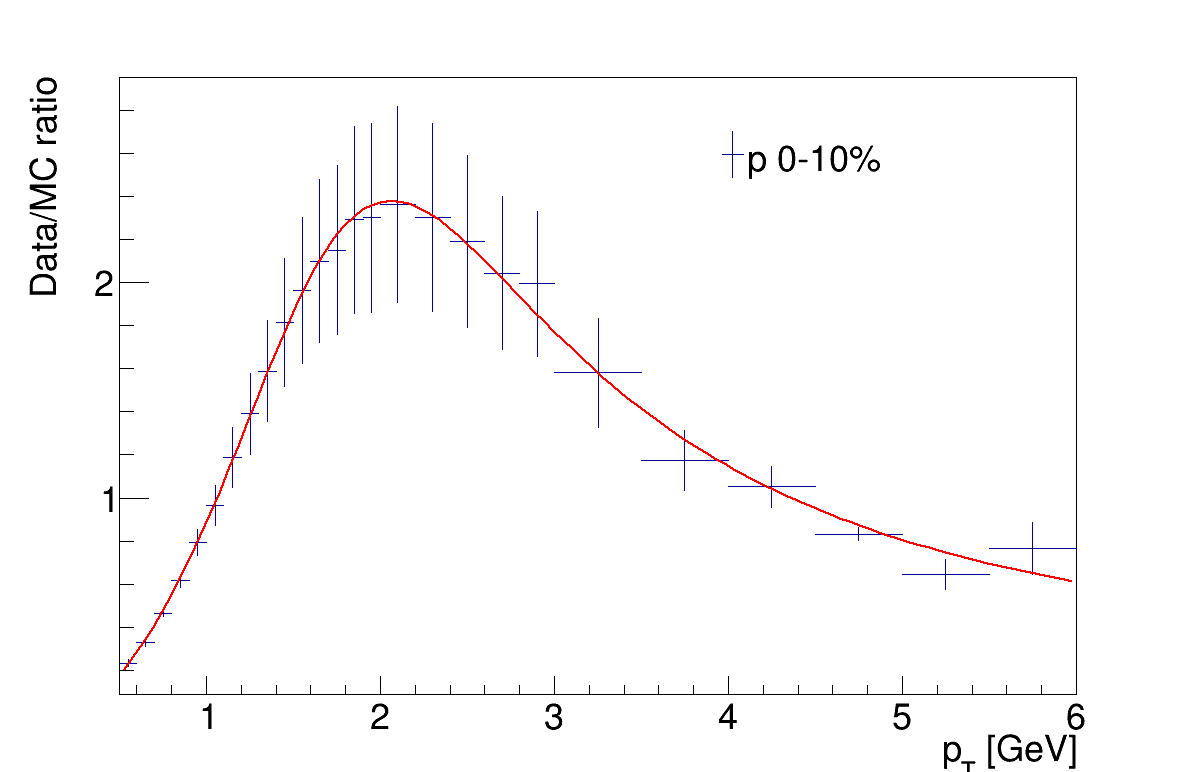
\includegraphics[width=0.24\linewidth]{detdeta/Figures/particle_reweighting_ratios/HIJING_p_0.png}
    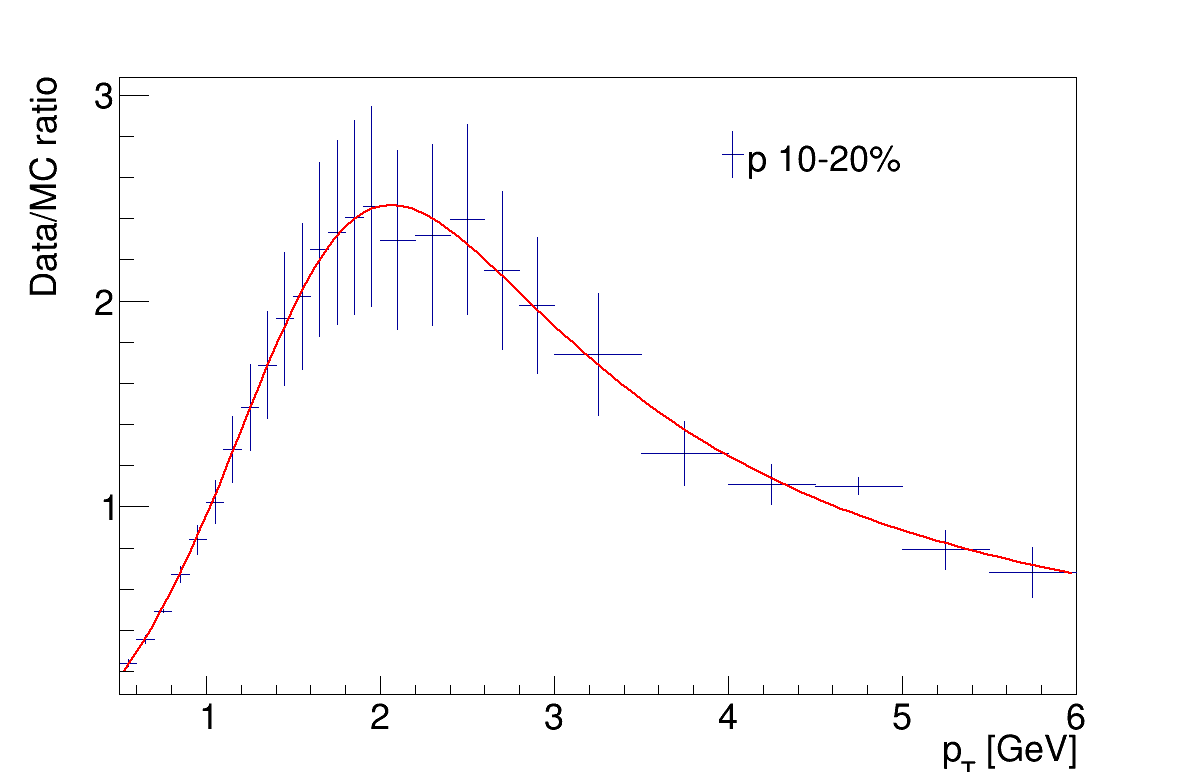
\includegraphics[width=0.24\linewidth]{detdeta/Figures/particle_reweighting_ratios/HIJING_p_1.png}
    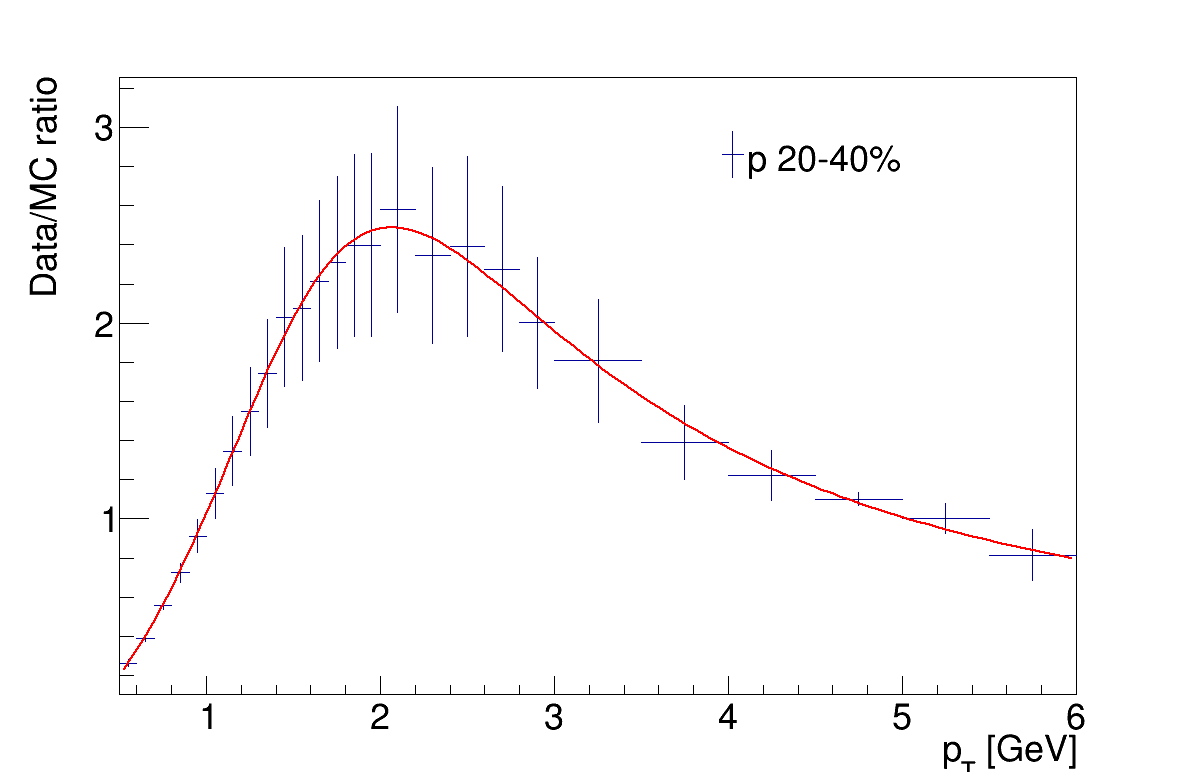
\includegraphics[width=0.24\linewidth]{detdeta/Figures/particle_reweighting_ratios/HIJING_p_2.png}
    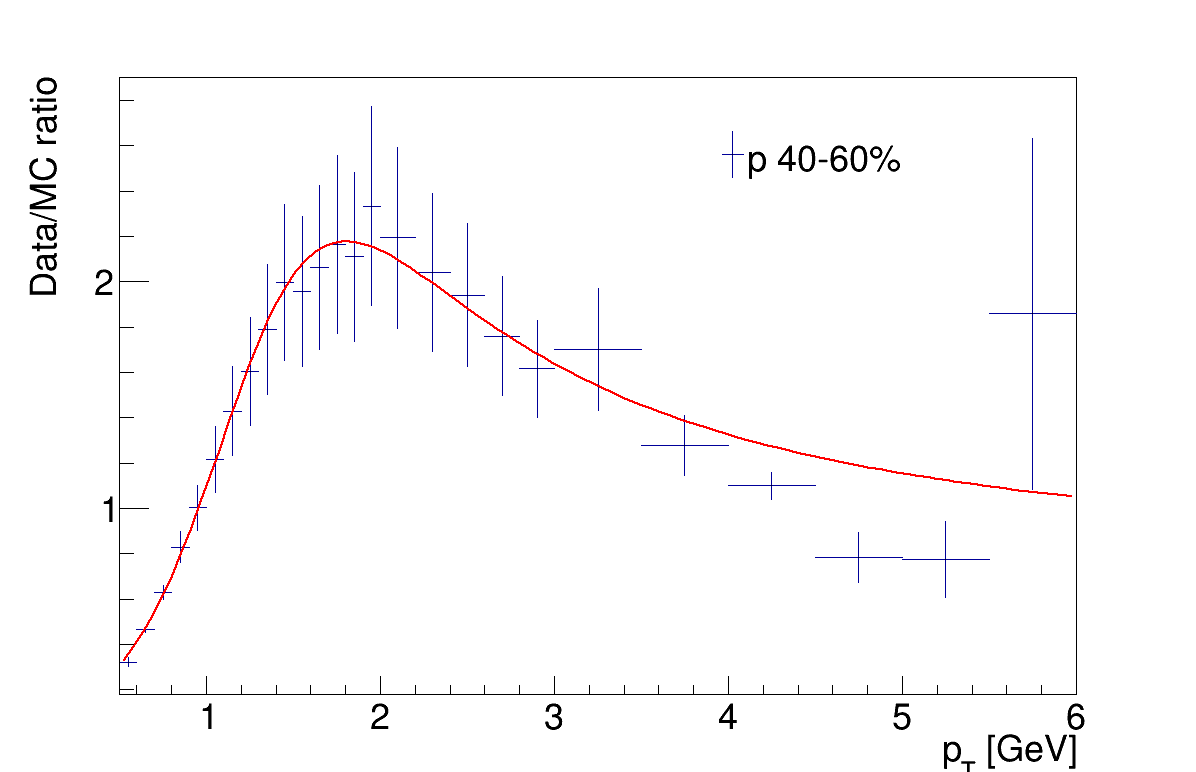
\includegraphics[width=0.24\linewidth]{detdeta/Figures/particle_reweighting_ratios/HIJING_p_3.png}
    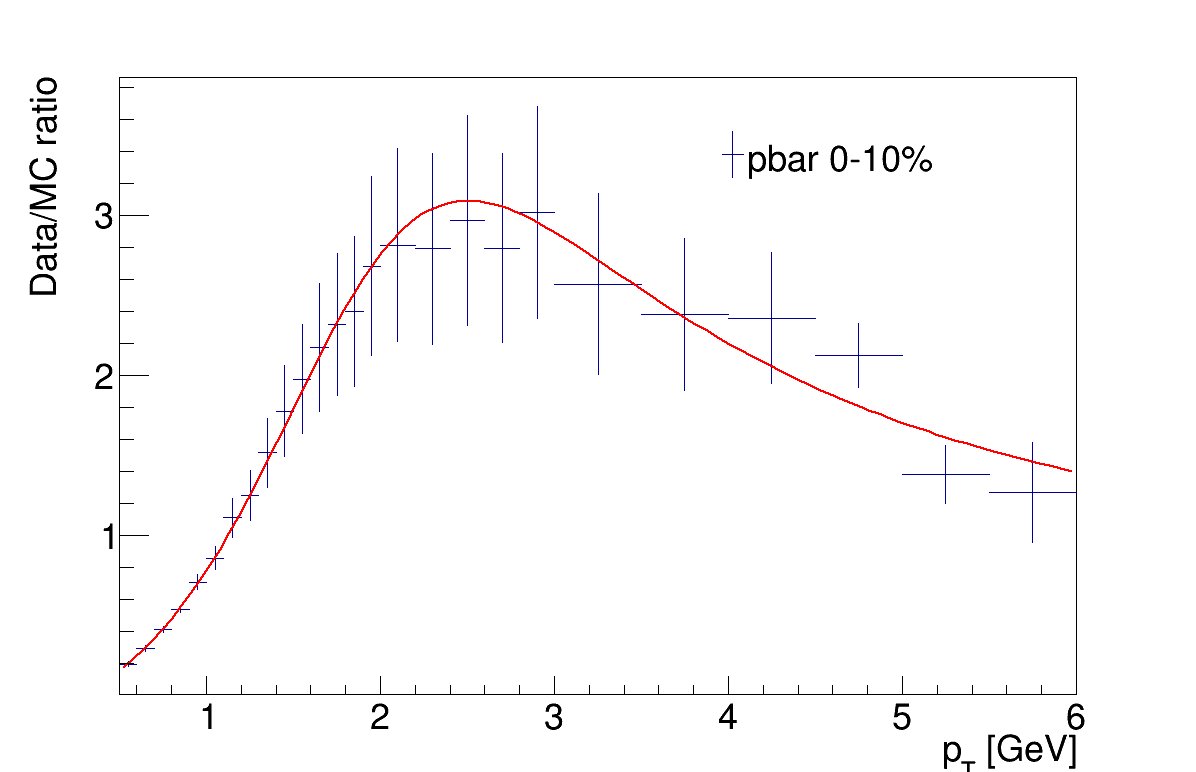
\includegraphics[width=0.24\linewidth]{detdeta/Figures/particle_reweighting_ratios/HIJING_pbar_0.png}
    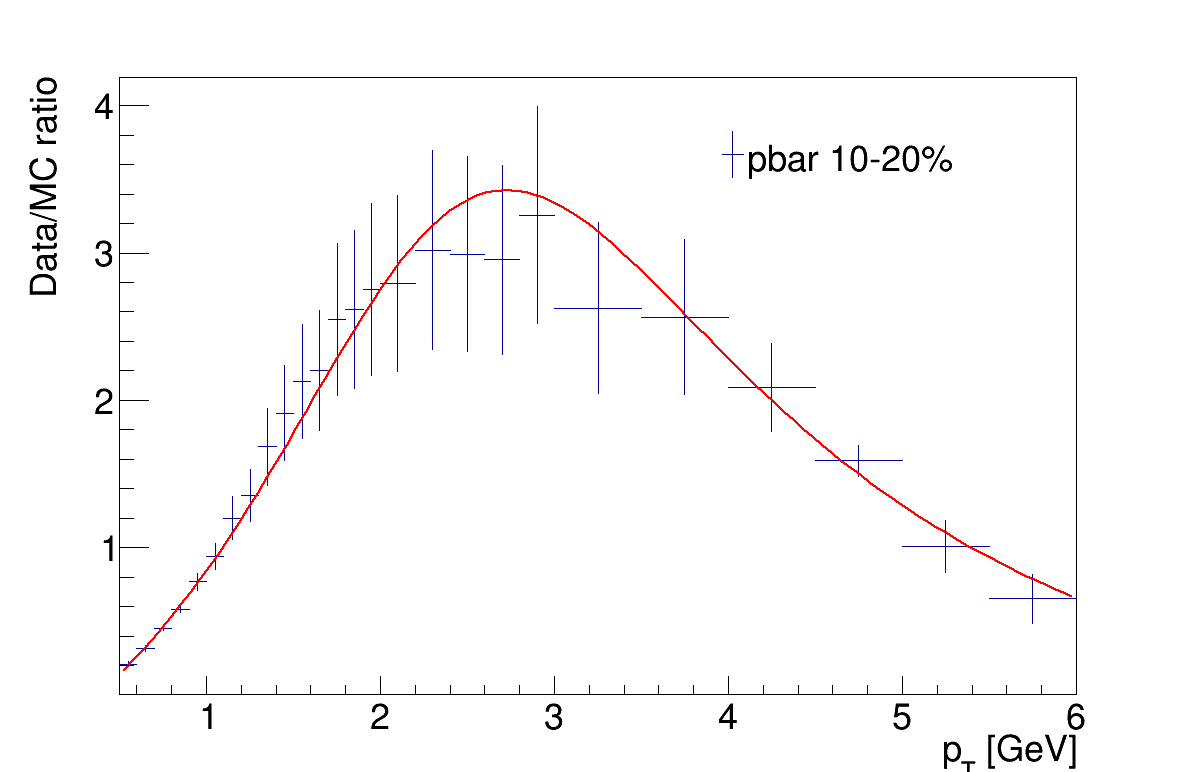
\includegraphics[width=0.24\linewidth]{detdeta/Figures/particle_reweighting_ratios/HIJING_pbar_1.png}
    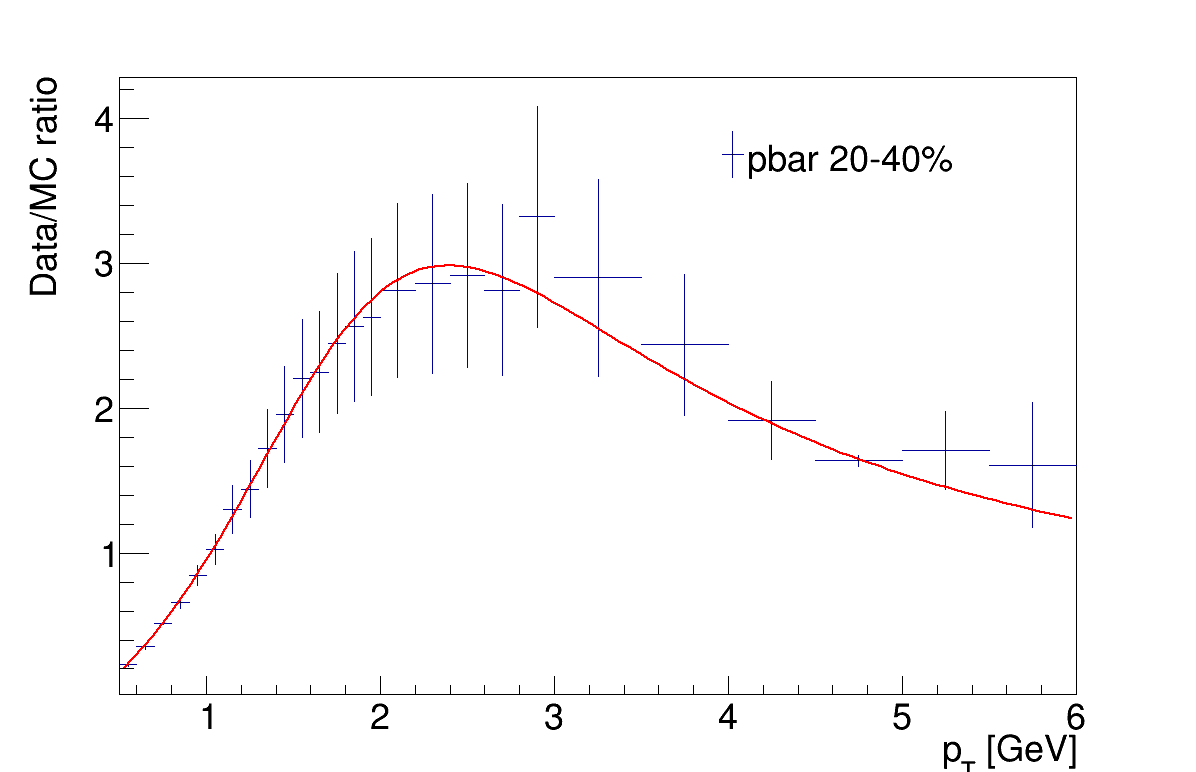
\includegraphics[width=0.24\linewidth]{detdeta/Figures/particle_reweighting_ratios/HIJING_pbar_2.png}
    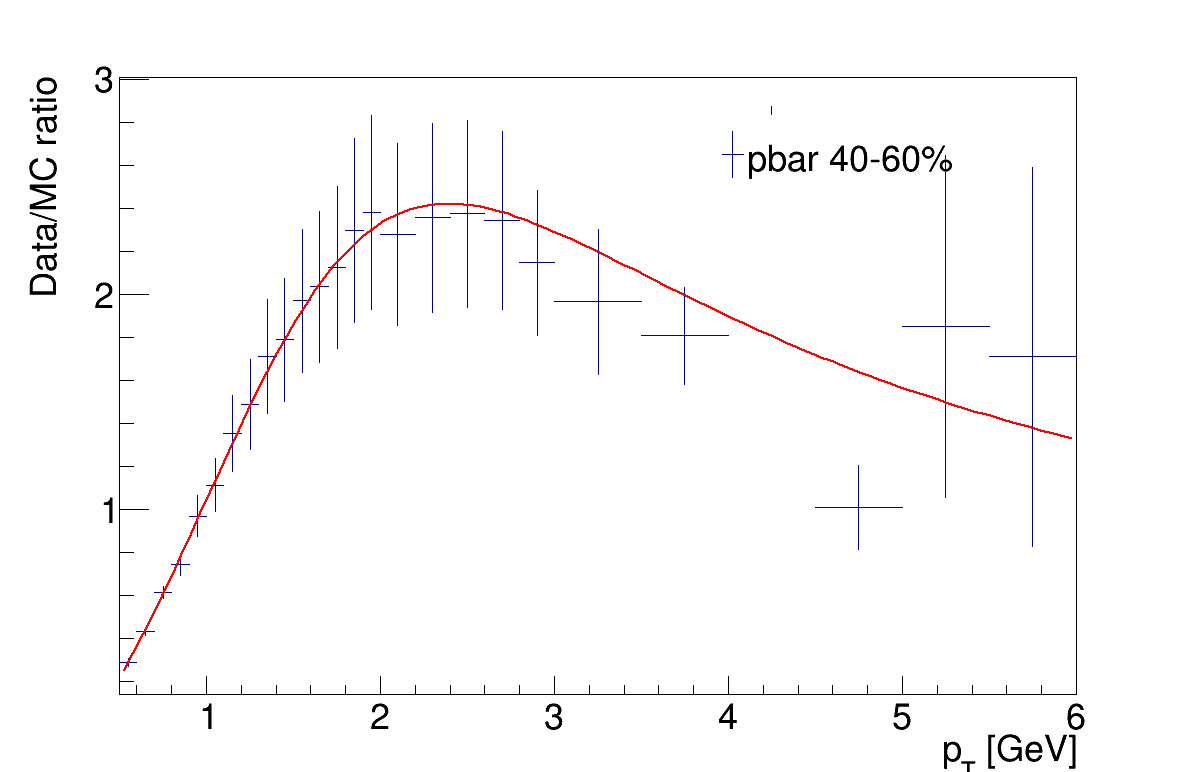
\includegraphics[width=0.24\linewidth]{detdeta/Figures/particle_reweighting_ratios/HIJING_pbar_3.png}
    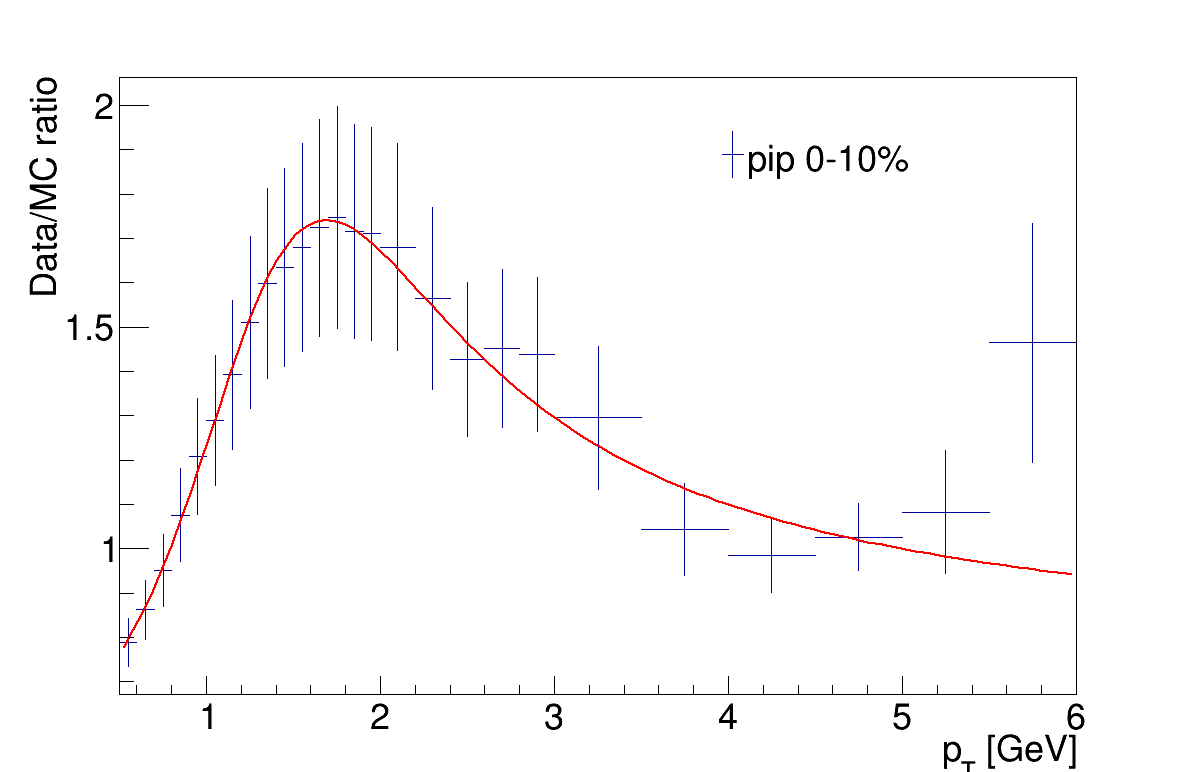
\includegraphics[width=0.24\linewidth]{detdeta/Figures/particle_reweighting_ratios/HIJING_pip_0.png}
    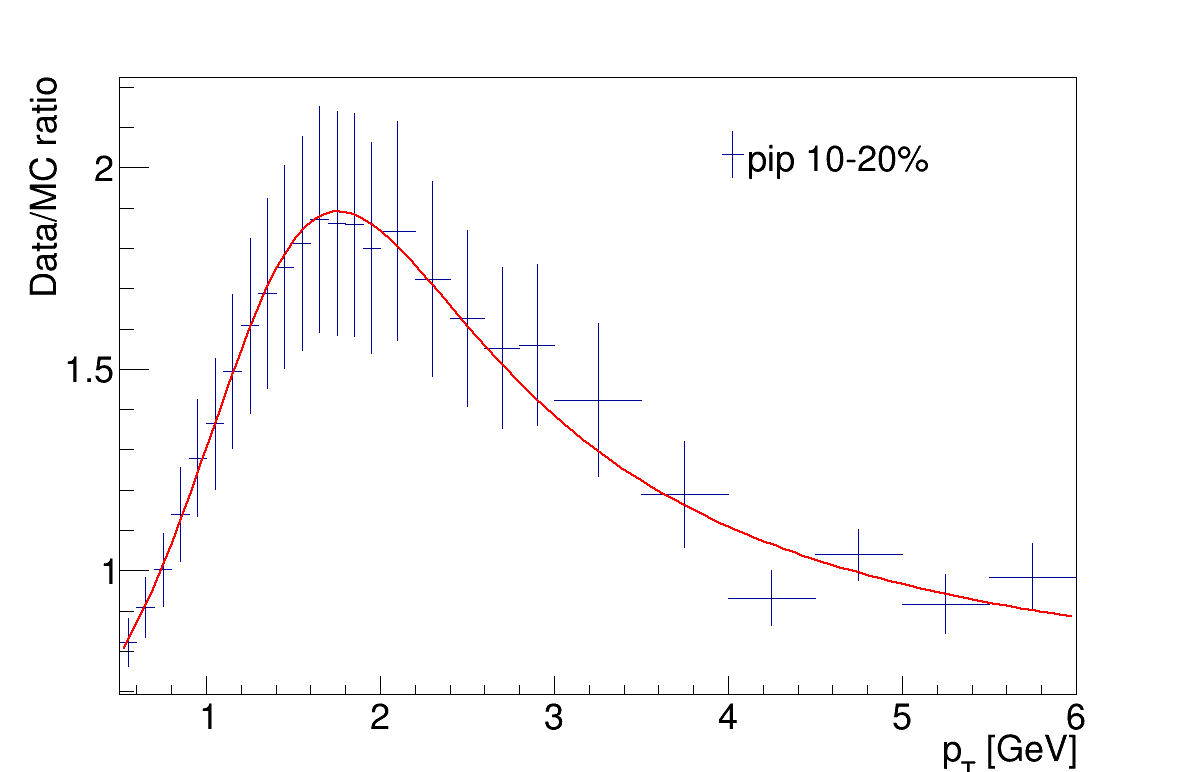
\includegraphics[width=0.24\linewidth]{detdeta/Figures/particle_reweighting_ratios/HIJING_pip_1.png}
    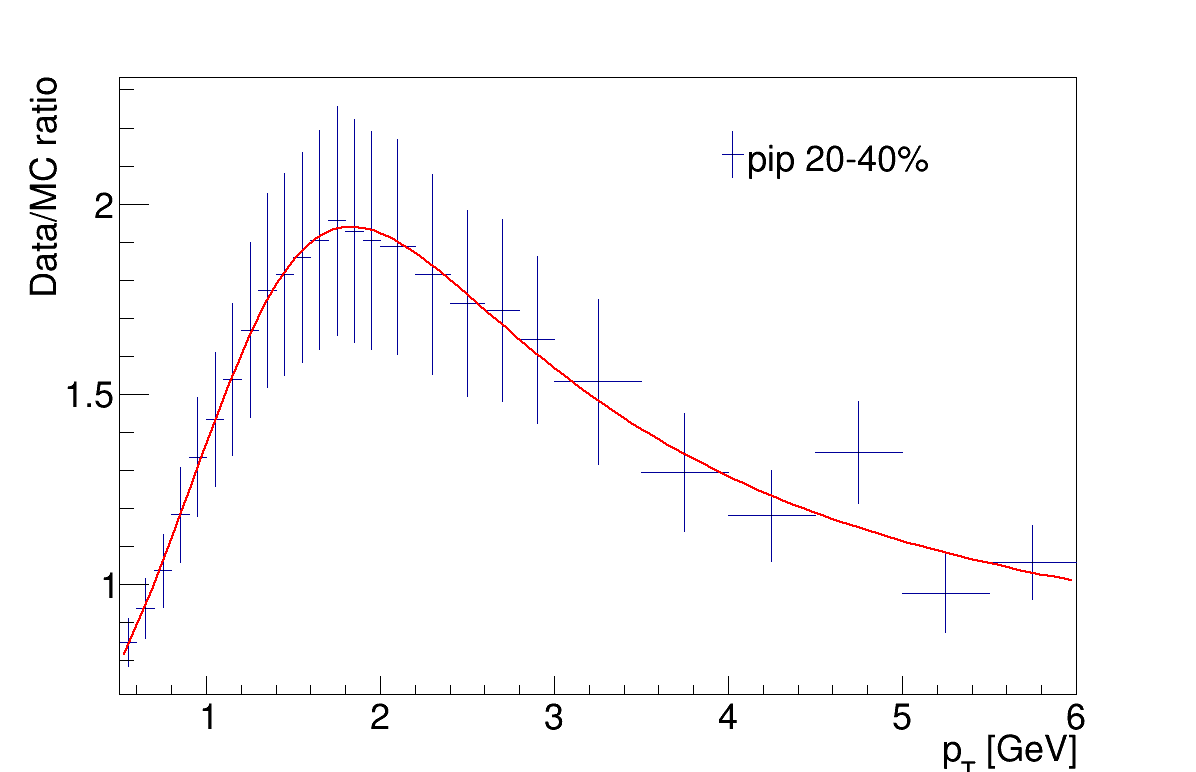
\includegraphics[width=0.24\linewidth]{detdeta/Figures/particle_reweighting_ratios/HIJING_pip_2.png}
    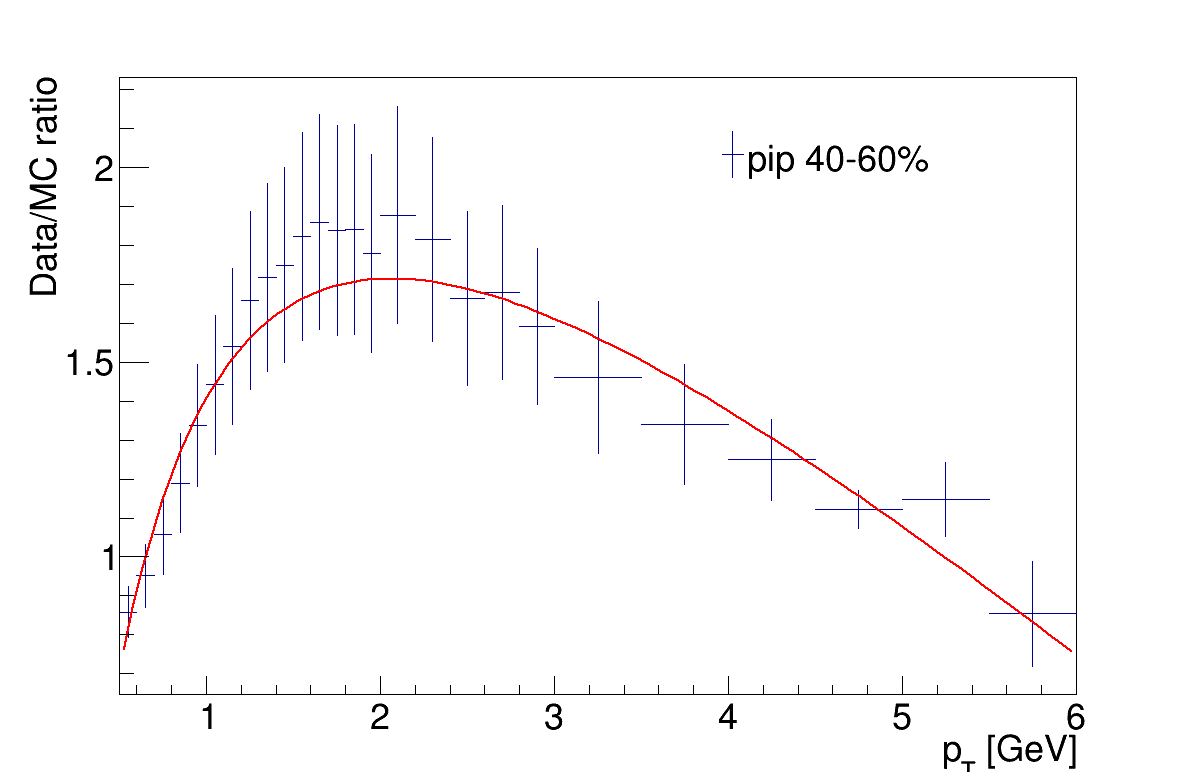
\includegraphics[width=0.24\linewidth]{detdeta/Figures/particle_reweighting_ratios/HIJING_pip_3.png}
    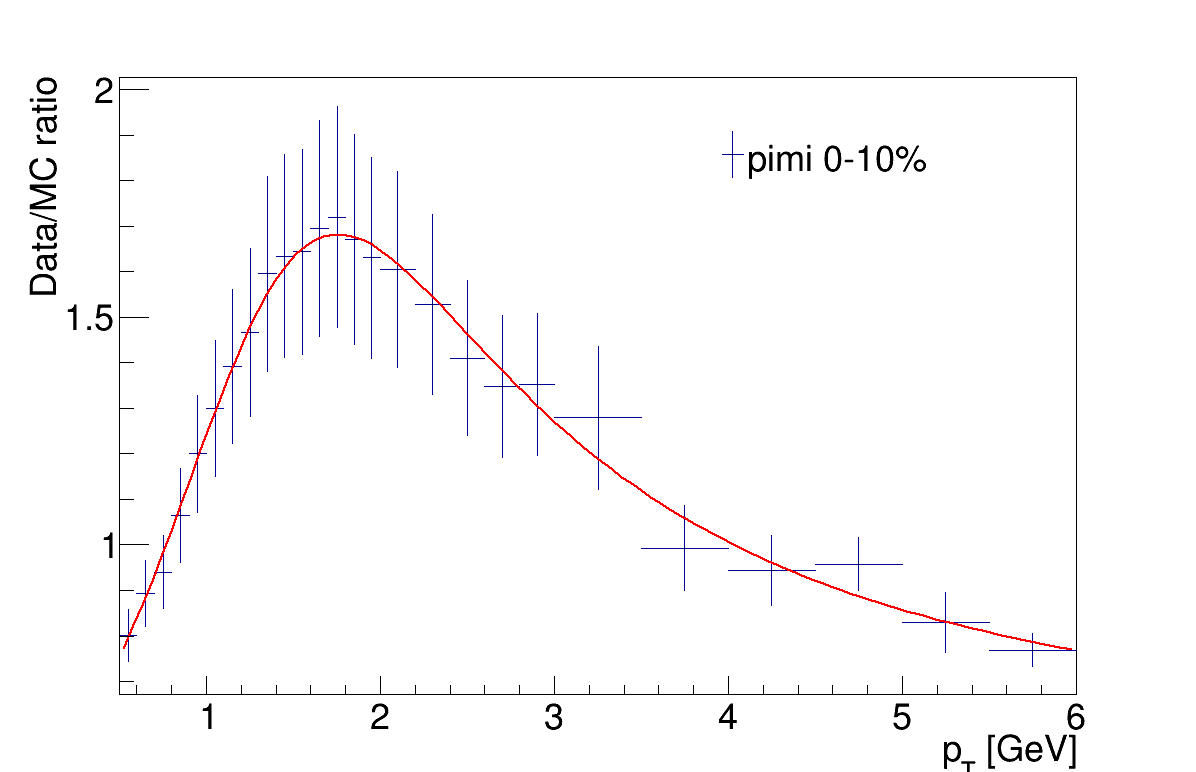
\includegraphics[width=0.24\linewidth]{detdeta/Figures/particle_reweighting_ratios/HIJING_pimi_0.png}
    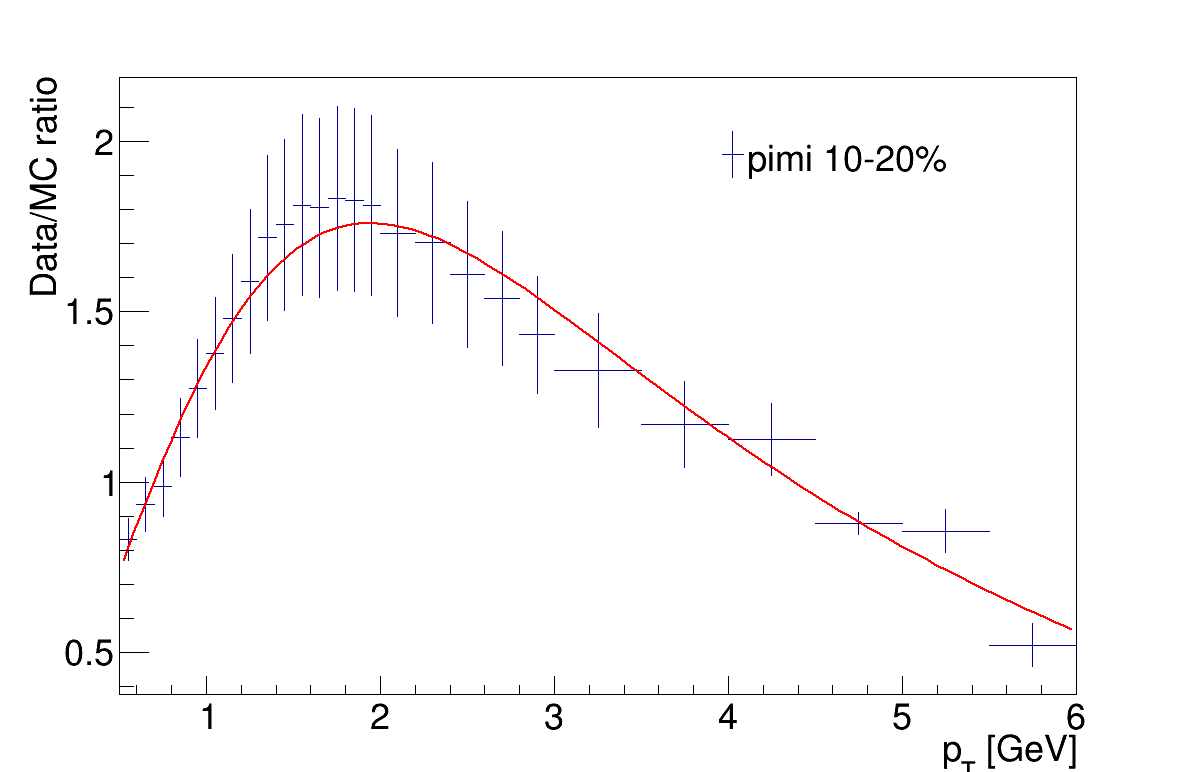
\includegraphics[width=0.24\linewidth]{detdeta/Figures/particle_reweighting_ratios/HIJING_pimi_1.png}
    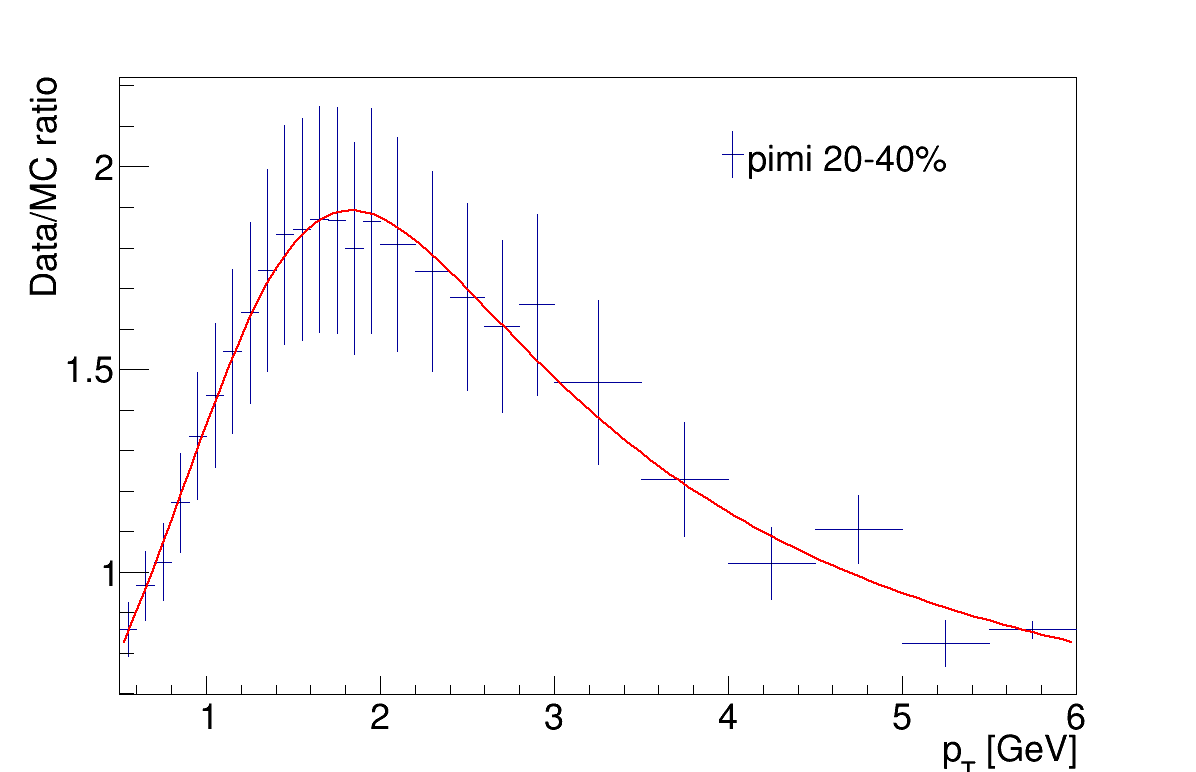
\includegraphics[width=0.24\linewidth]{detdeta/Figures/particle_reweighting_ratios/HIJING_pimi_2.png}
    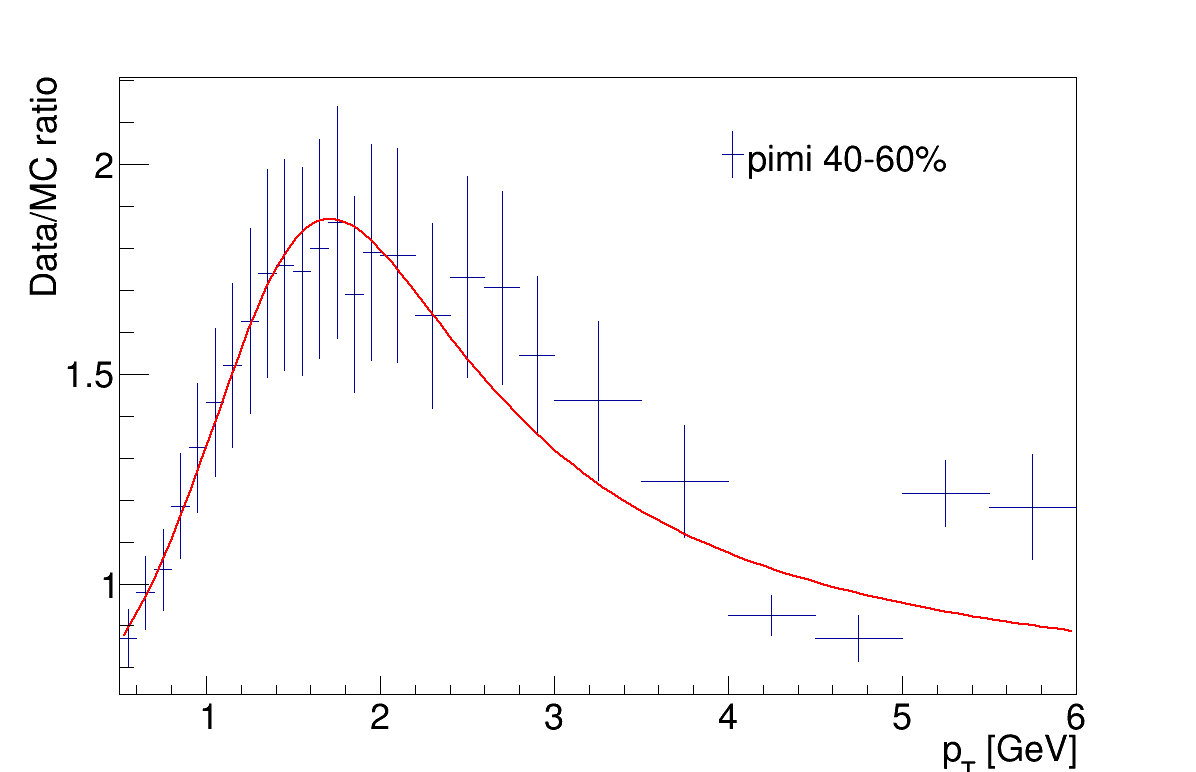
\includegraphics[width=0.24\linewidth]{detdeta/Figures/particle_reweighting_ratios/HIJING_pimi_3.png}
    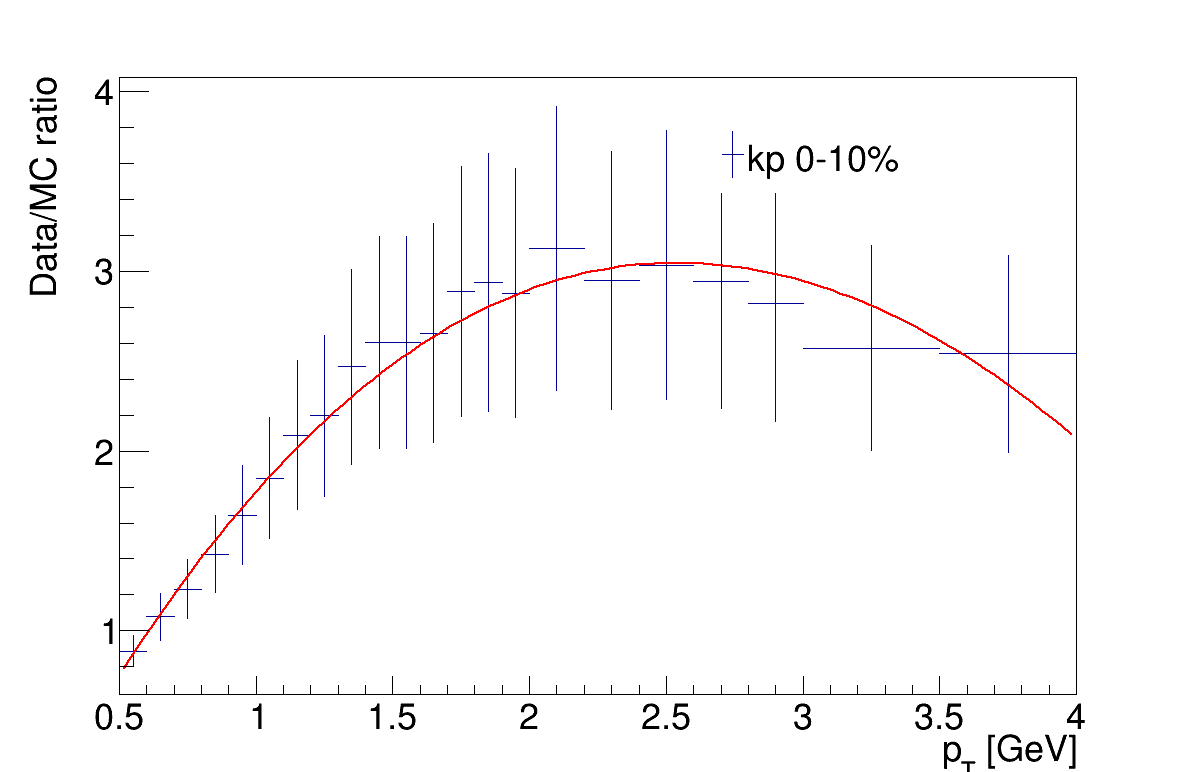
\includegraphics[width=0.24\linewidth]{detdeta/Figures/particle_reweighting_ratios/HIJING_kp_0.png}
    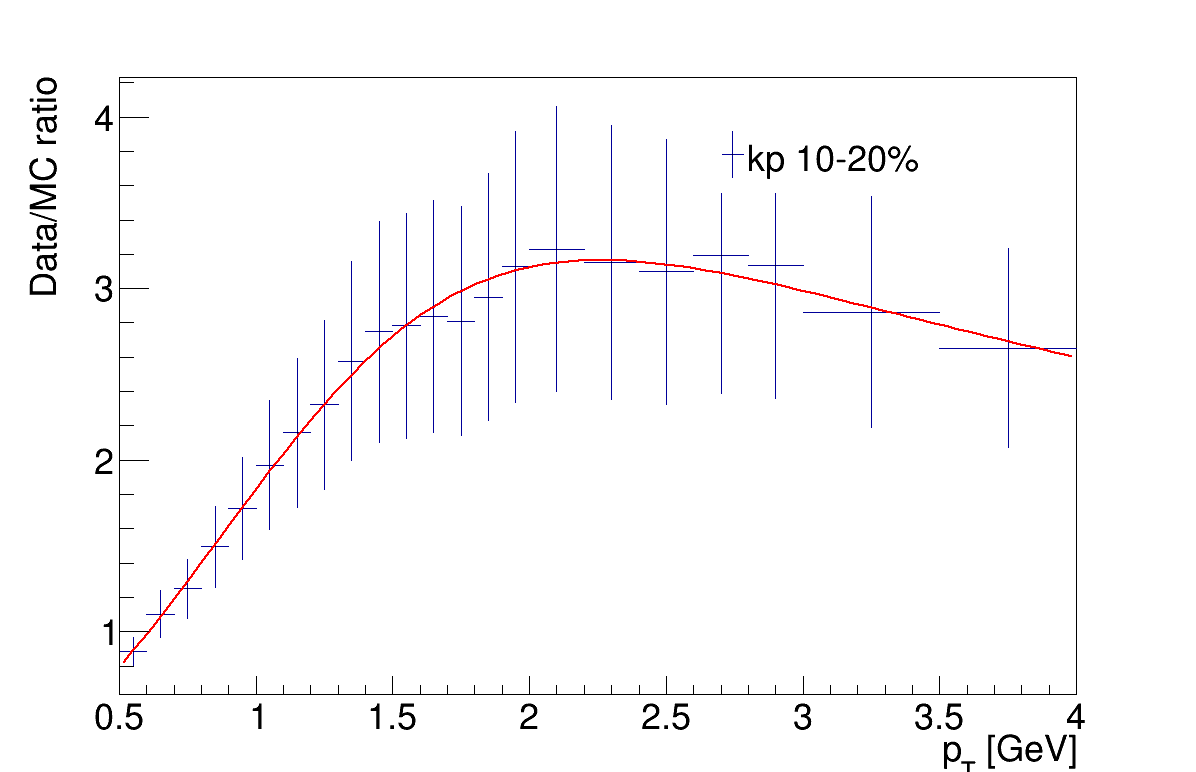
\includegraphics[width=0.24\linewidth]{detdeta/Figures/particle_reweighting_ratios/HIJING_kp_1.png}
    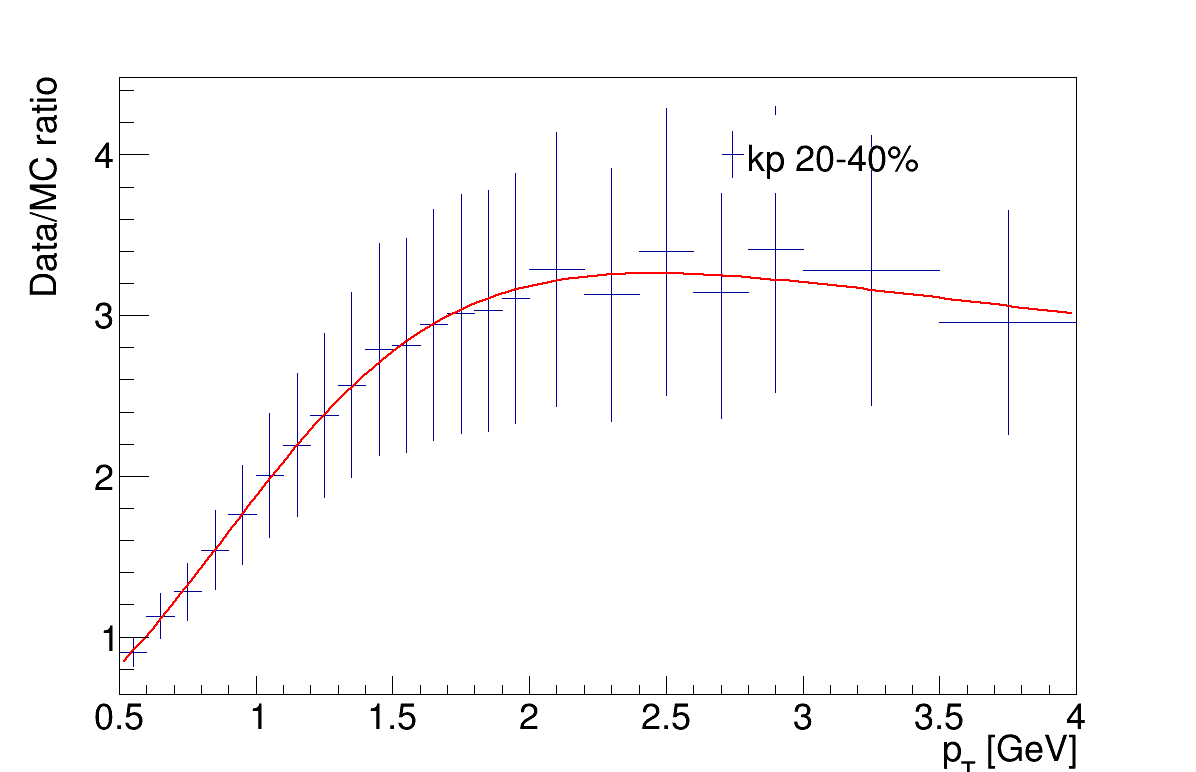
\includegraphics[width=0.24\linewidth]{detdeta/Figures/particle_reweighting_ratios/HIJING_kp_2.png}
    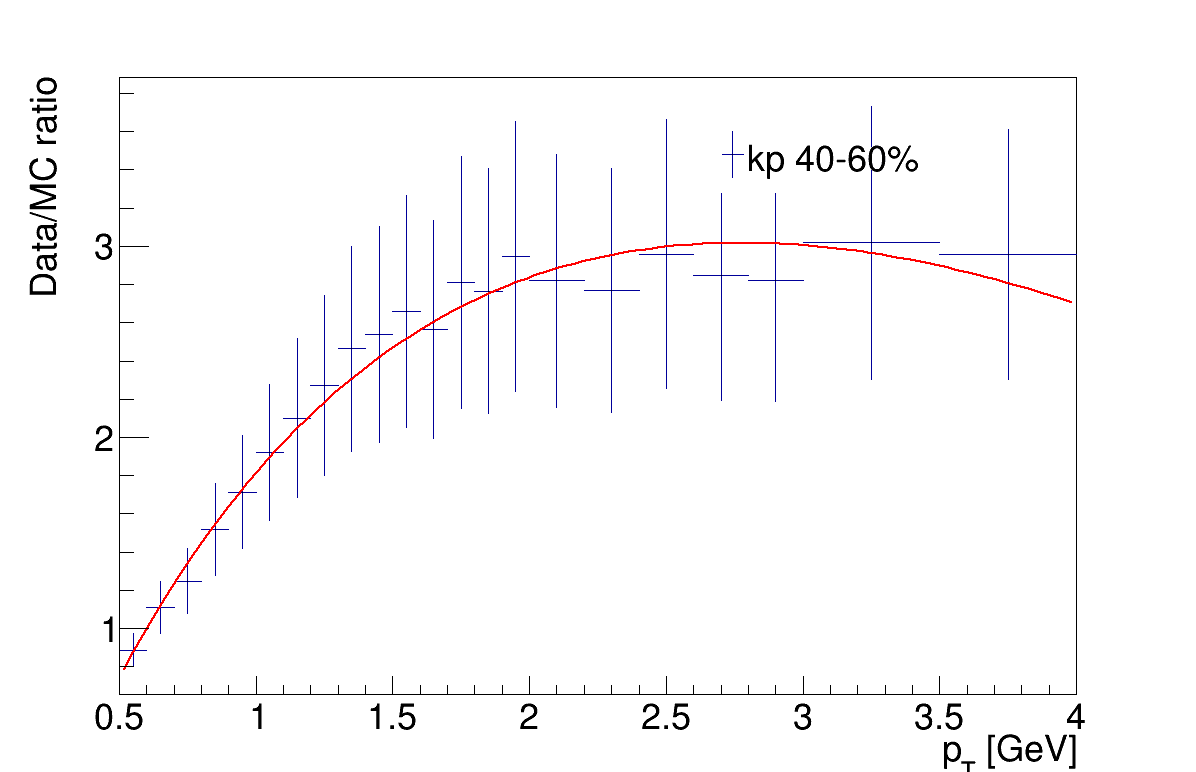
\includegraphics[width=0.24\linewidth]{detdeta/Figures/particle_reweighting_ratios/HIJING_kp_3.png}
    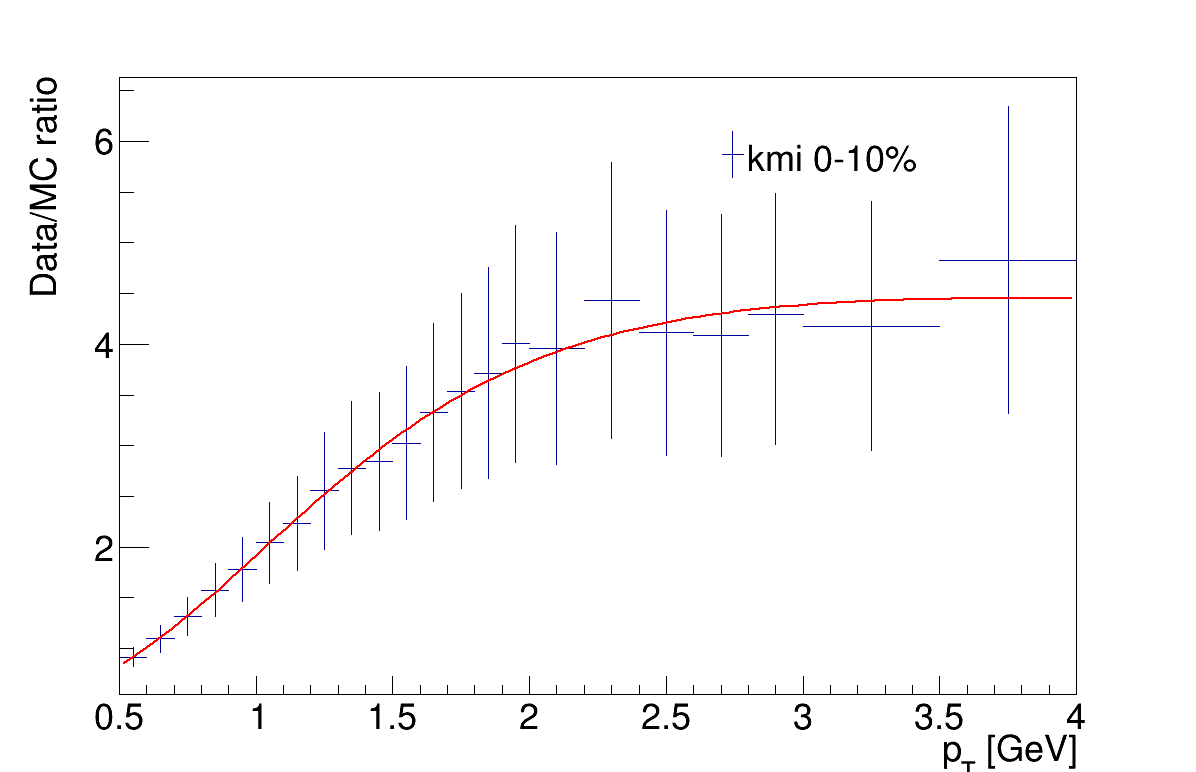
\includegraphics[width=0.24\linewidth]{detdeta/Figures/particle_reweighting_ratios/HIJING_kmi_0.png}
    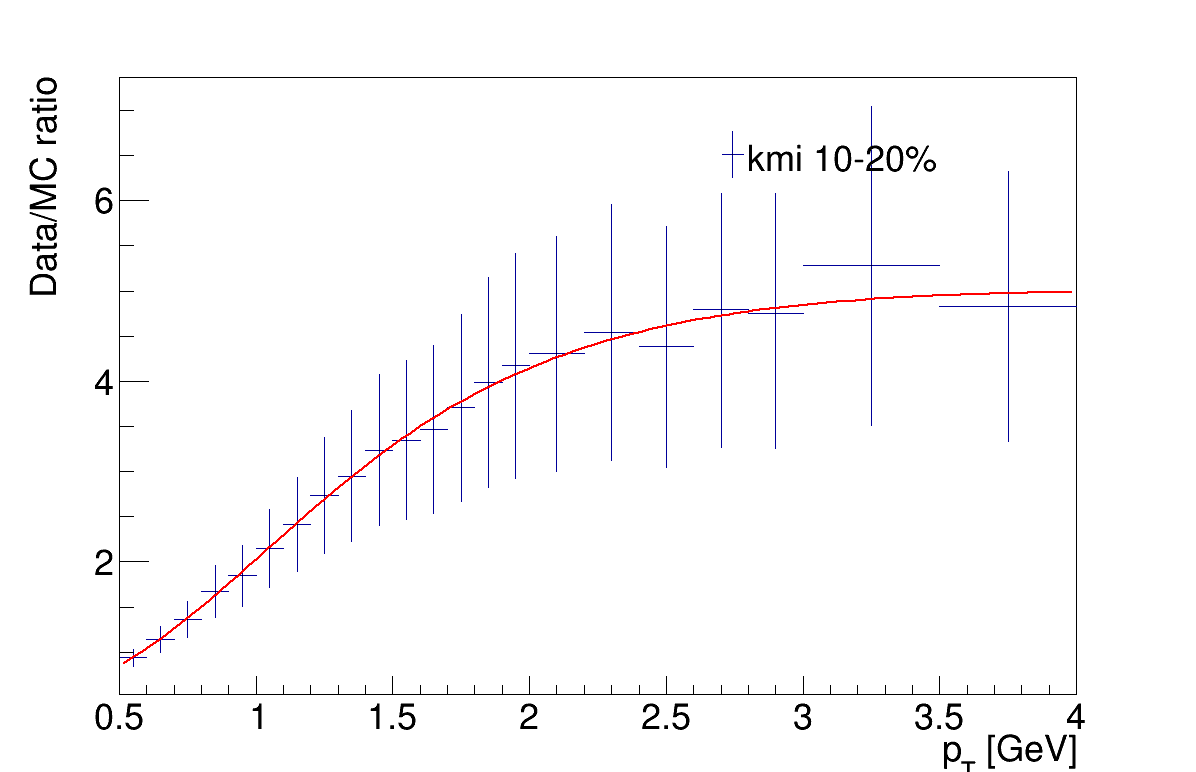
\includegraphics[width=0.24\linewidth]{detdeta/Figures/particle_reweighting_ratios/HIJING_kmi_1.png}
    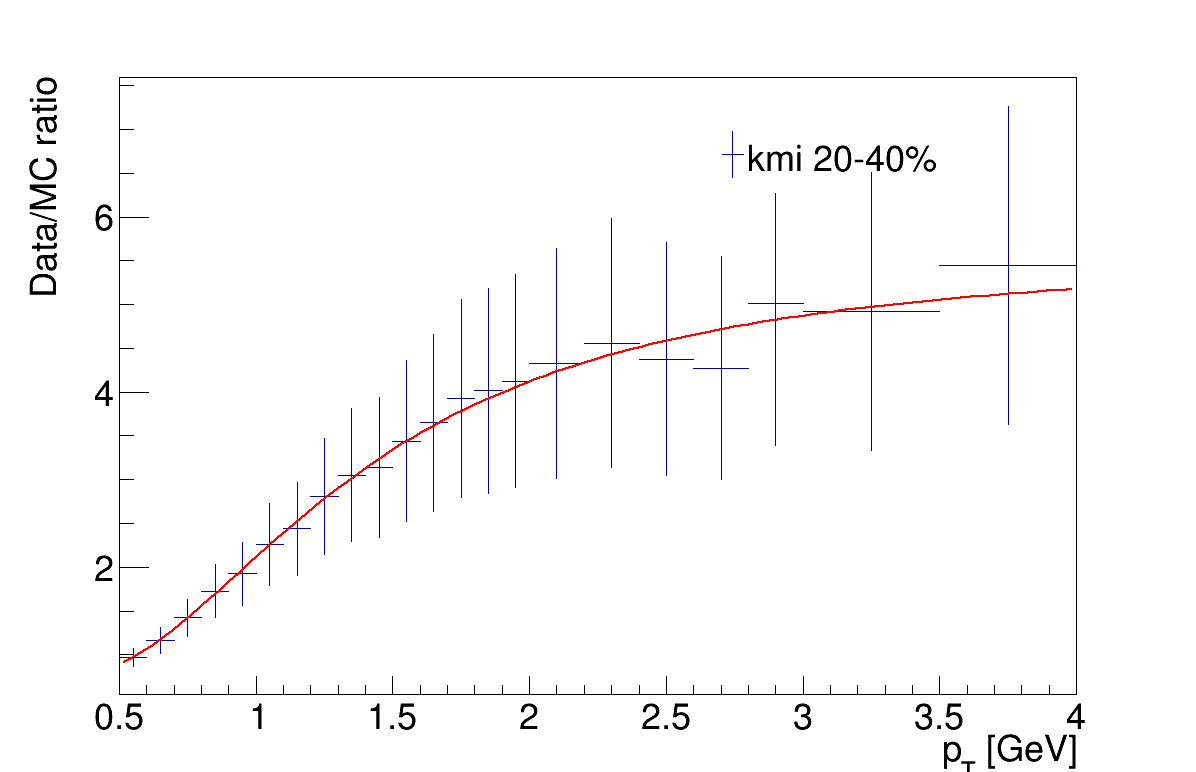
\includegraphics[width=0.24\linewidth]{detdeta/Figures/particle_reweighting_ratios/HIJING_kmi_2.png}
    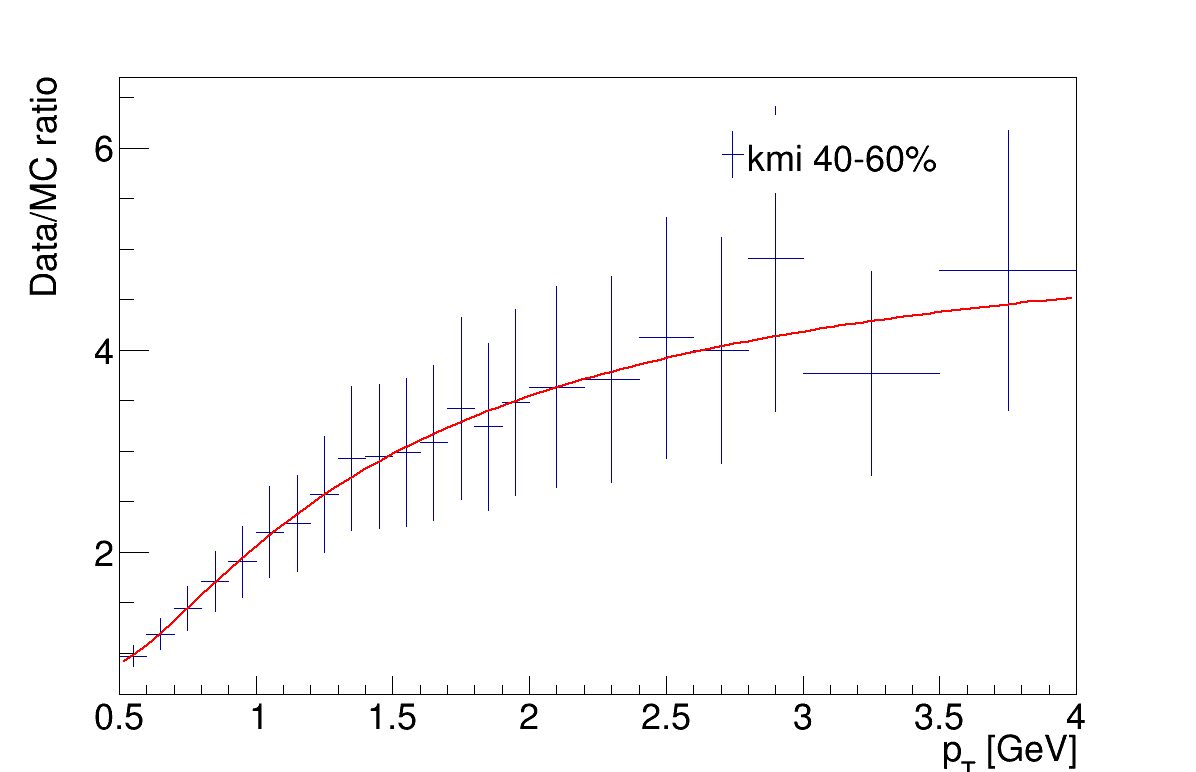
\includegraphics[width=0.24\linewidth]{detdeta/Figures/particle_reweighting_ratios/HIJING_kmi_3.png}
    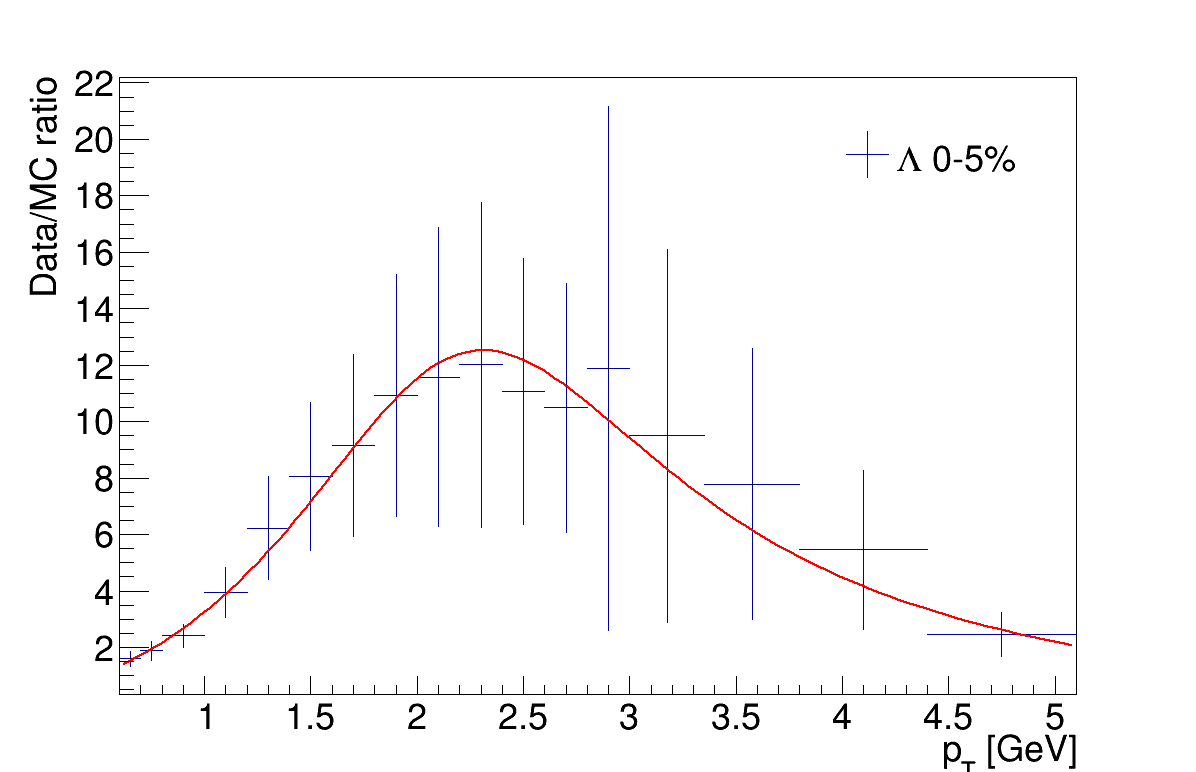
\includegraphics[width=0.24\linewidth]{detdeta/Figures/particle_reweighting_ratios/HIJING_lambda_0.png}
    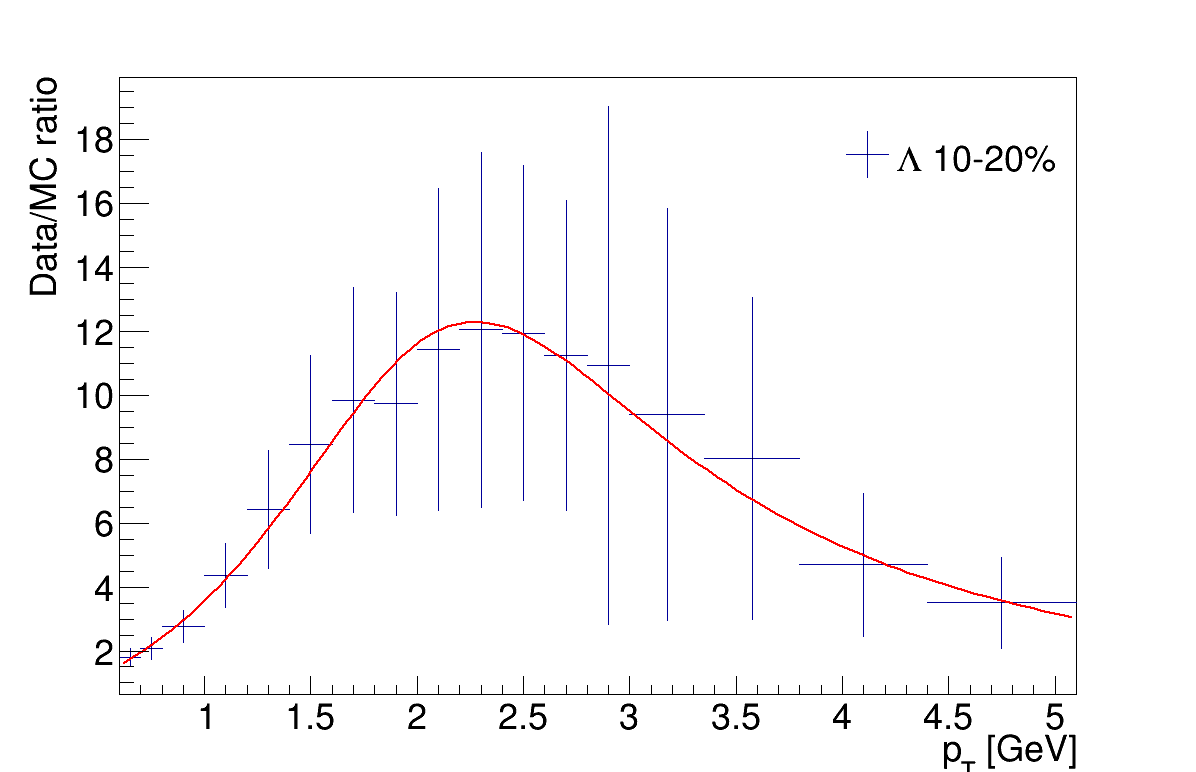
\includegraphics[width=0.24\linewidth]{detdeta/Figures/particle_reweighting_ratios/HIJING_lambda_1.png}
    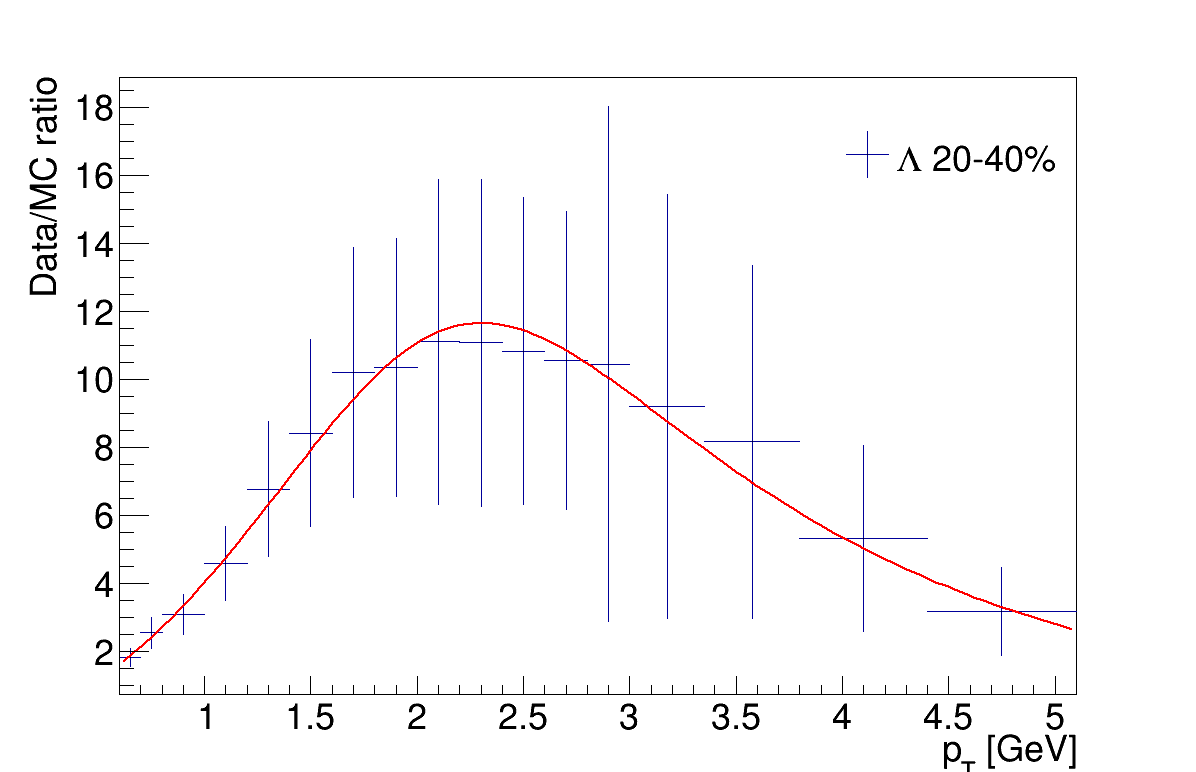
\includegraphics[width=0.24\linewidth]{detdeta/Figures/particle_reweighting_ratios/HIJING_lambda_2.png}
    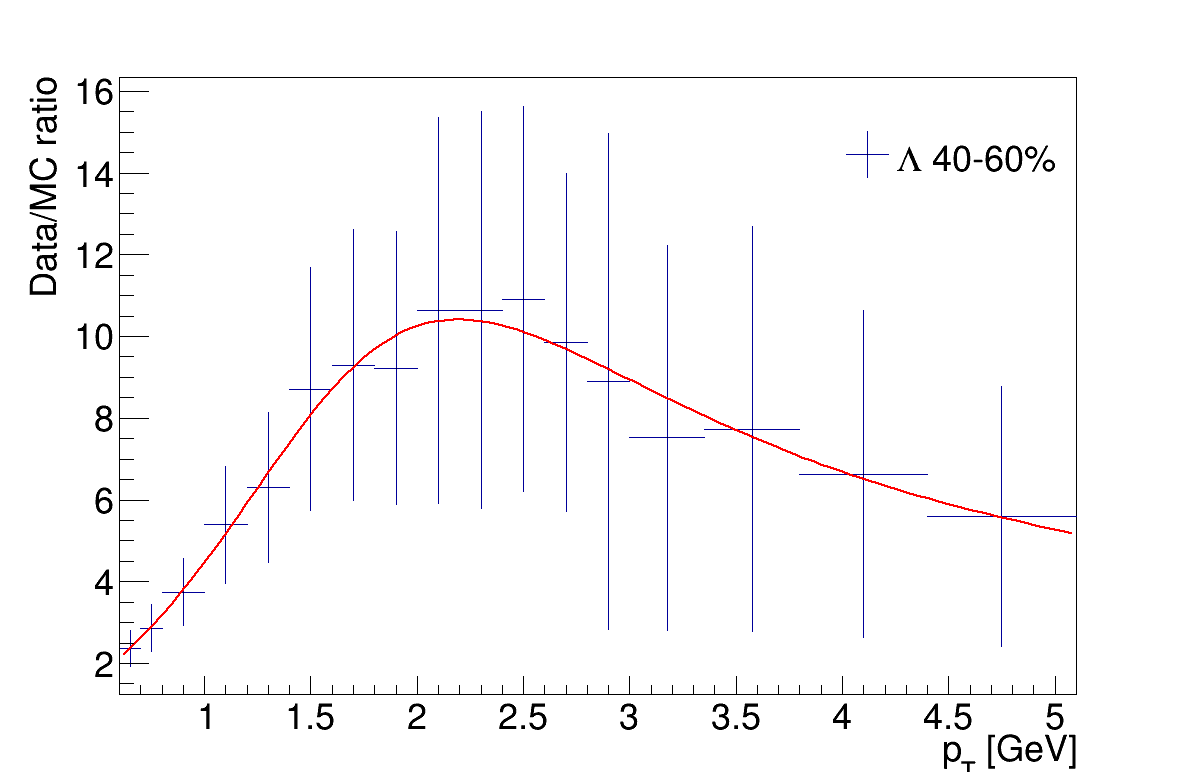
\includegraphics[width=0.24\linewidth]{detdeta/Figures/particle_reweighting_ratios/HIJING_lambda_3.png}
    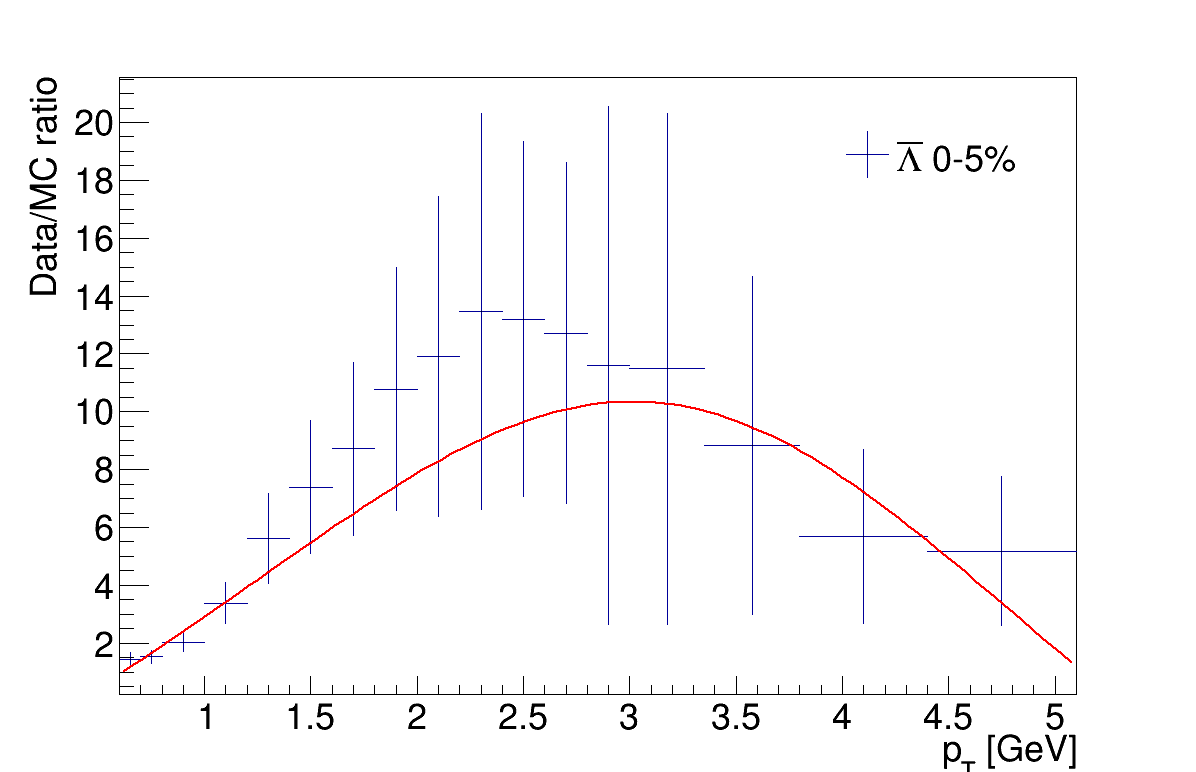
\includegraphics[width=0.24\linewidth]{detdeta/Figures/particle_reweighting_ratios/HIJING_lambda_bar_0.png}
    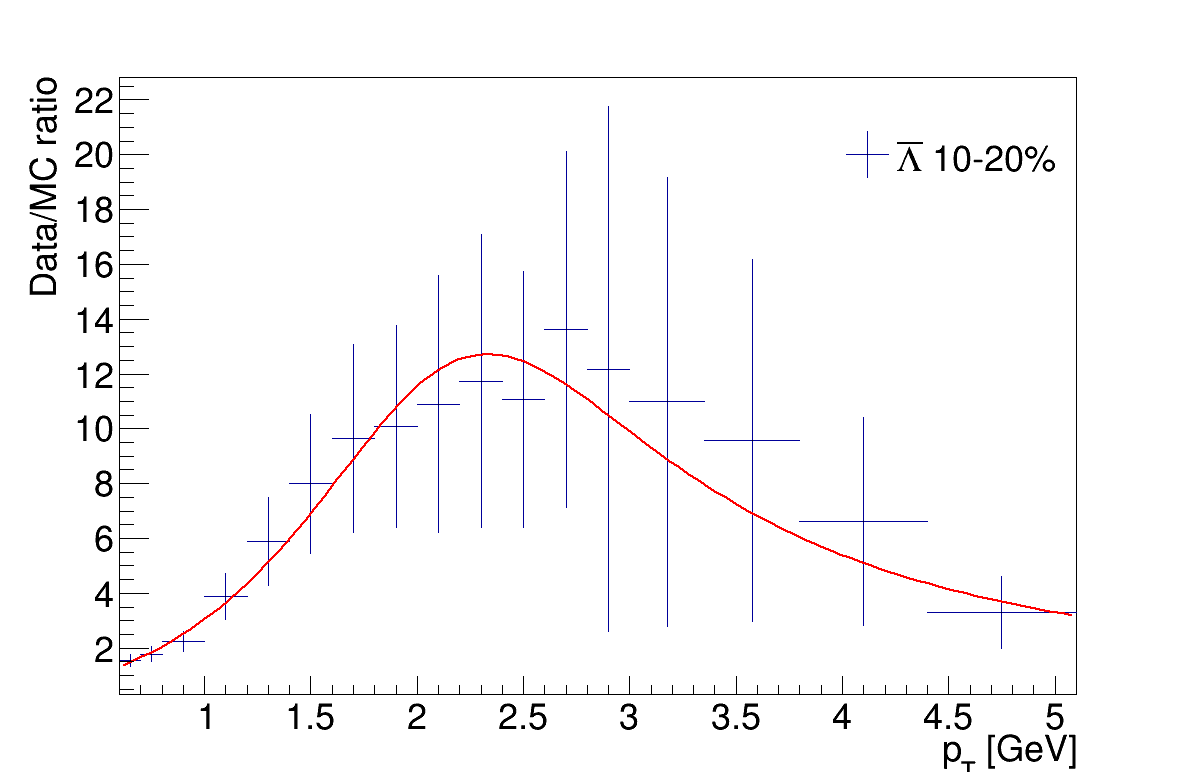
\includegraphics[width=0.24\linewidth]{detdeta/Figures/particle_reweighting_ratios/HIJING_lambda_bar_1.png}
    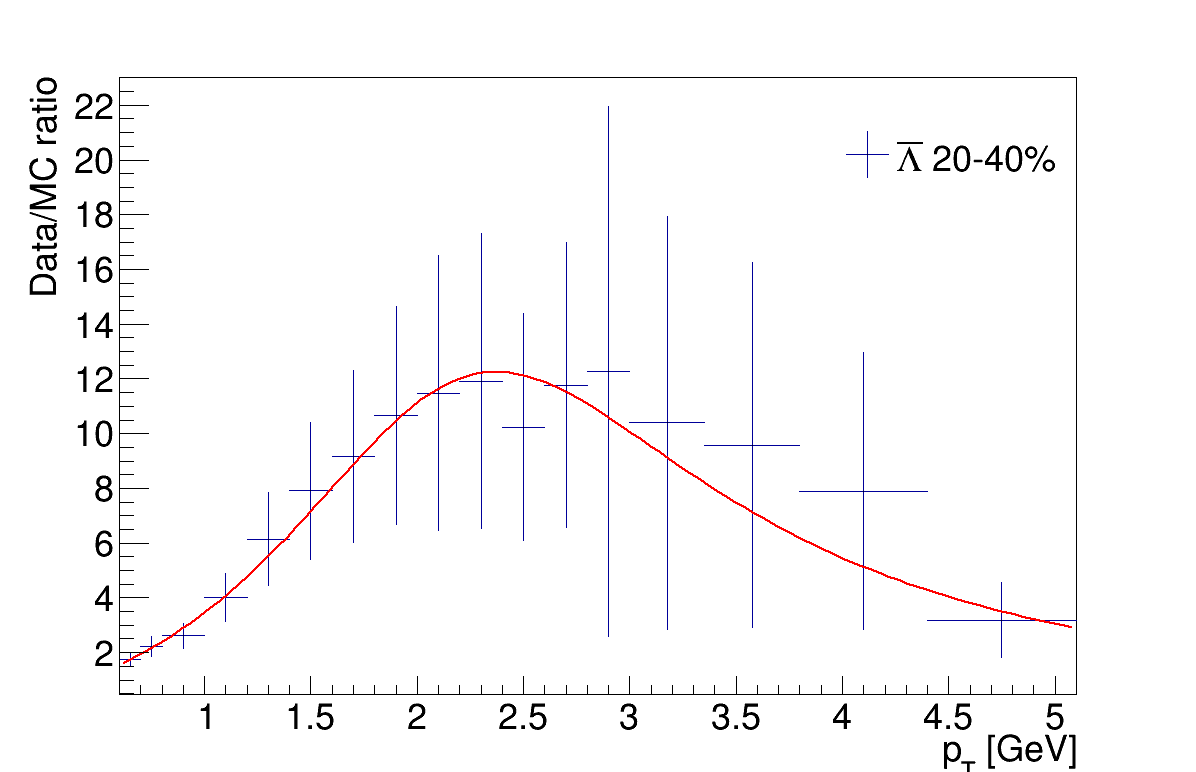
\includegraphics[width=0.24\linewidth]{detdeta/Figures/particle_reweighting_ratios/HIJING_lambda_bar_2.png}
    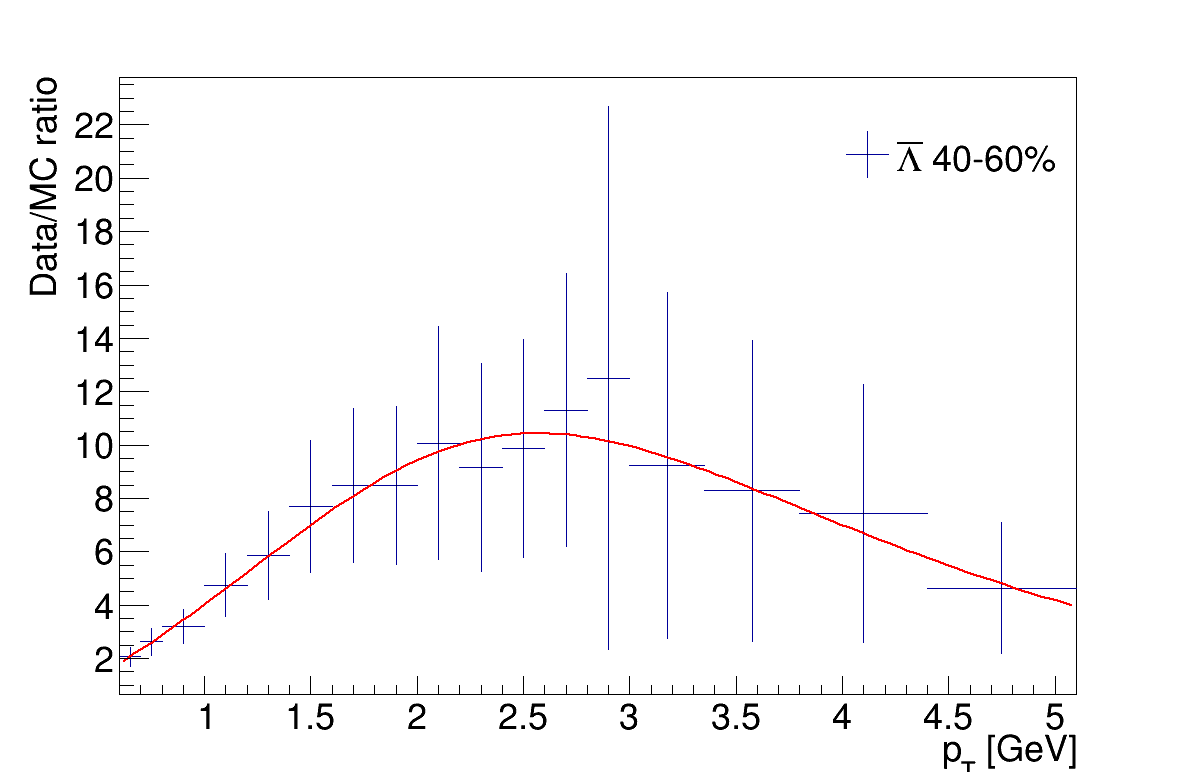
\includegraphics[width=0.24\linewidth]{detdeta/Figures/particle_reweighting_ratios/HIJING_lambda_bar_3.png}
    \caption{All data to MC ratios used in nominal HIJING reweighting method for protons, anti-protons, kaons, pions and lambda particles.}
    \label{fig:hijing_data_mc_particle_ratios}
\end{figure}

\begin{figure}
    \centering
    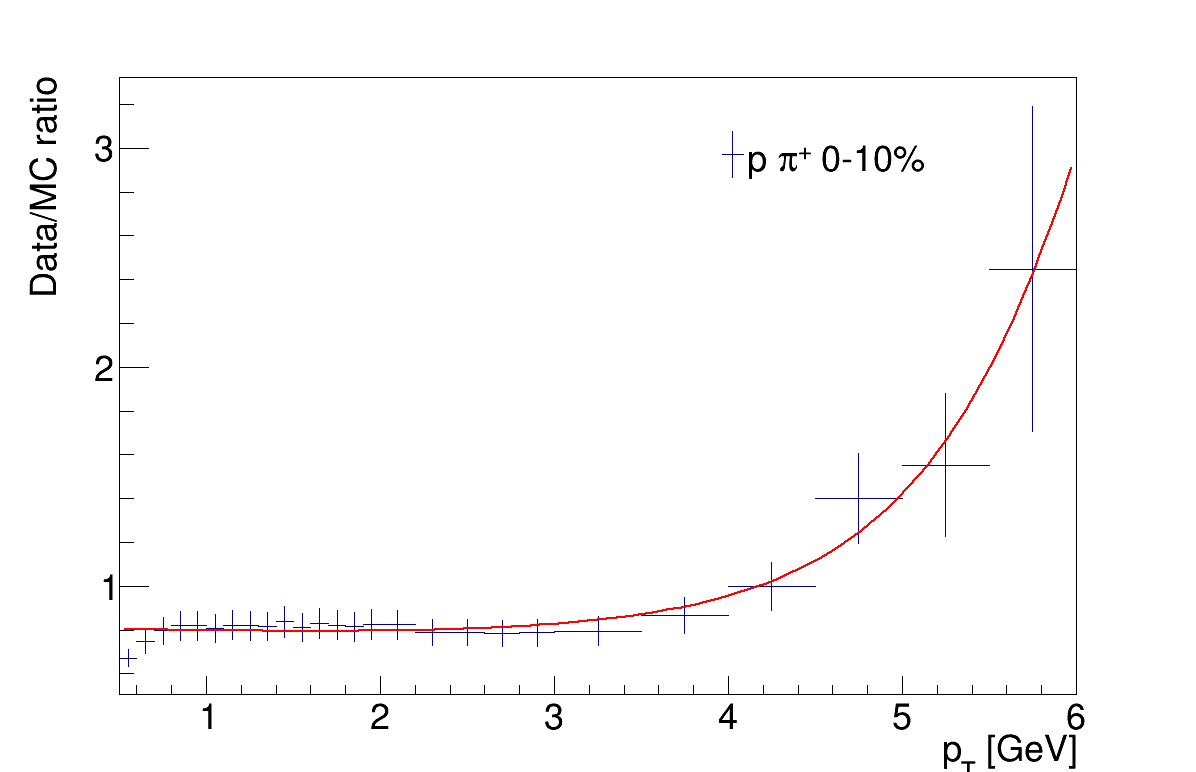
\includegraphics[width=0.24\linewidth]{detdeta/Figures/particle_reweighting_ratios/EPOS_p_0.png}
    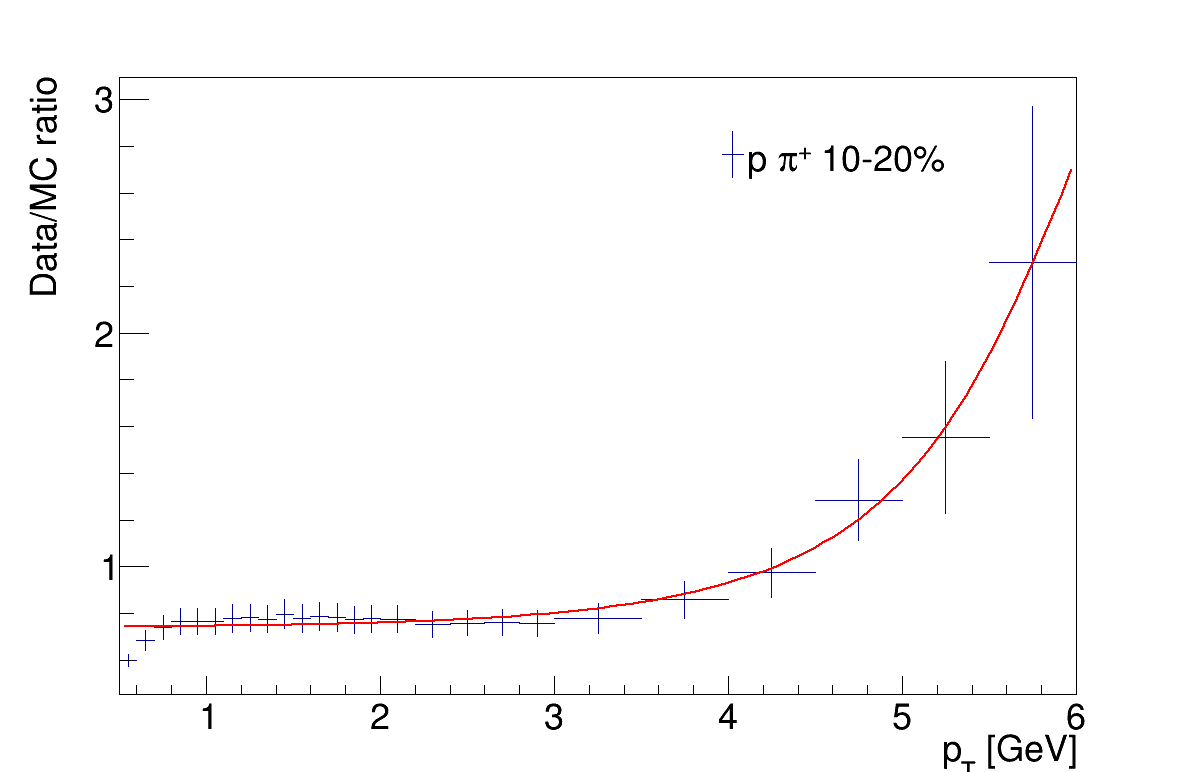
\includegraphics[width=0.24\linewidth]{detdeta/Figures/particle_reweighting_ratios/EPOS_p_1.png}
    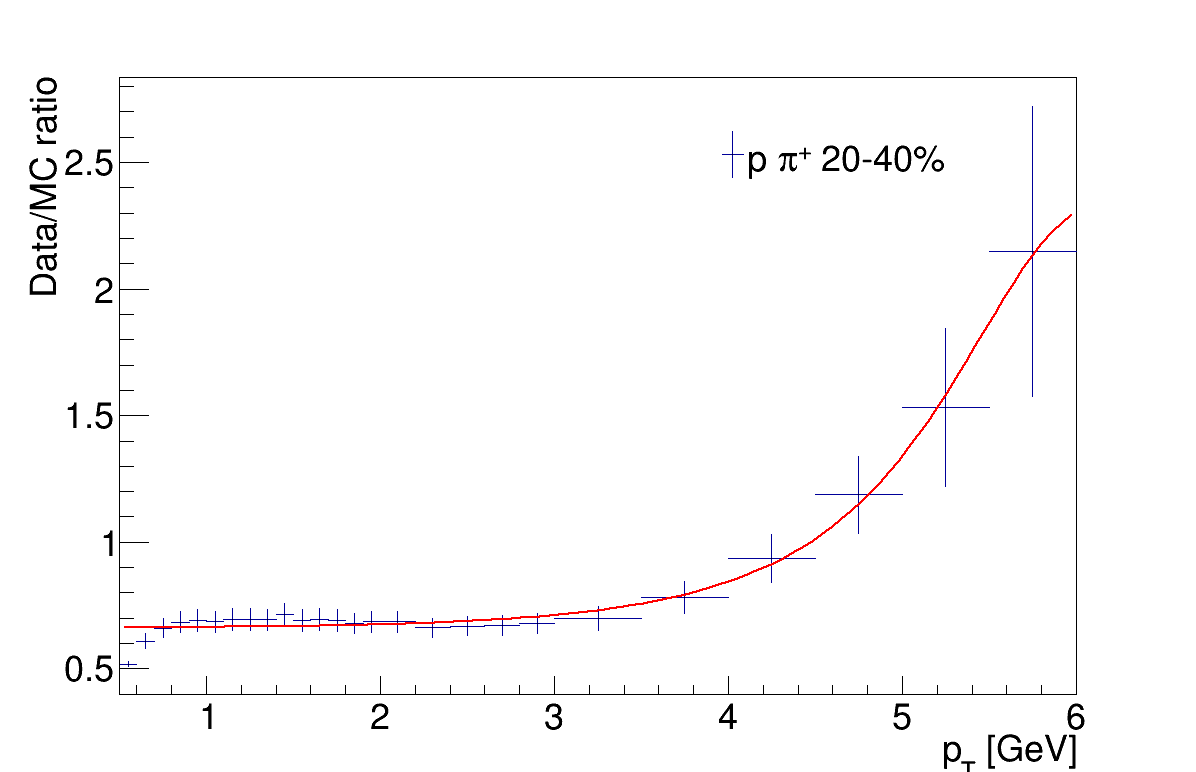
\includegraphics[width=0.24\linewidth]{detdeta/Figures/particle_reweighting_ratios/EPOS_p_2.png}
    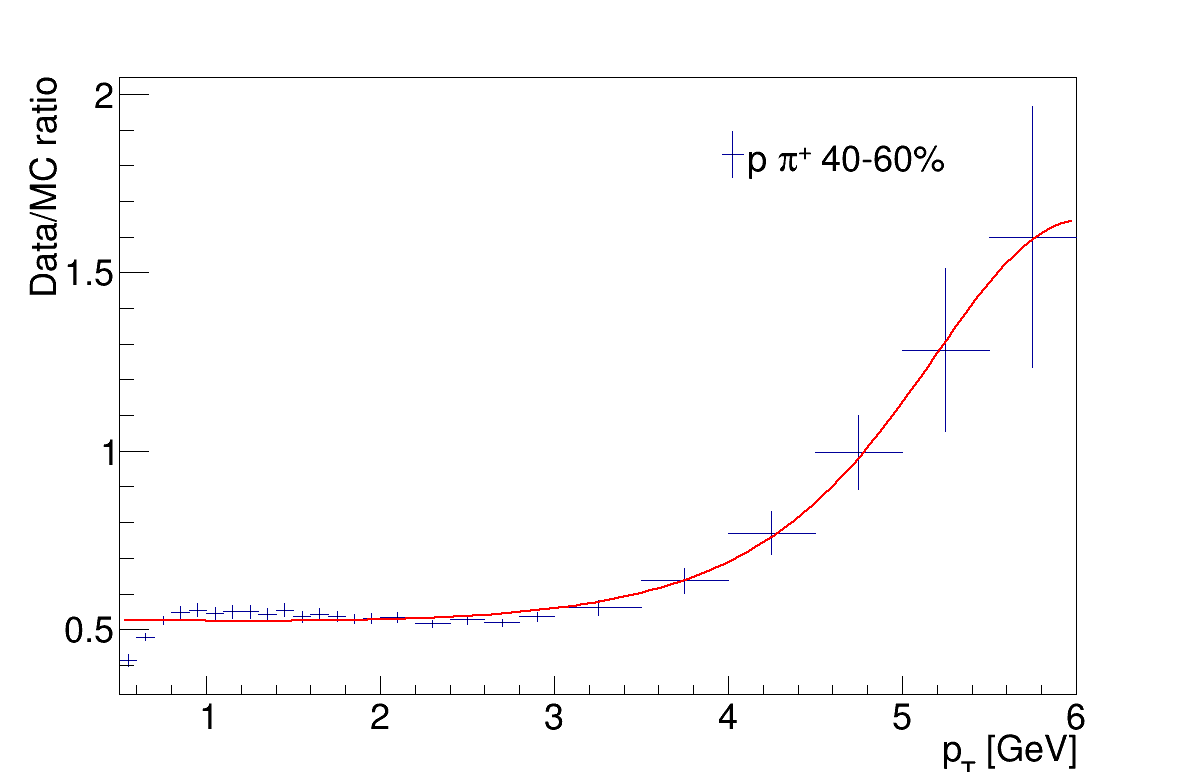
\includegraphics[width=0.24\linewidth]{detdeta/Figures/particle_reweighting_ratios/EPOS_p_3.png}
    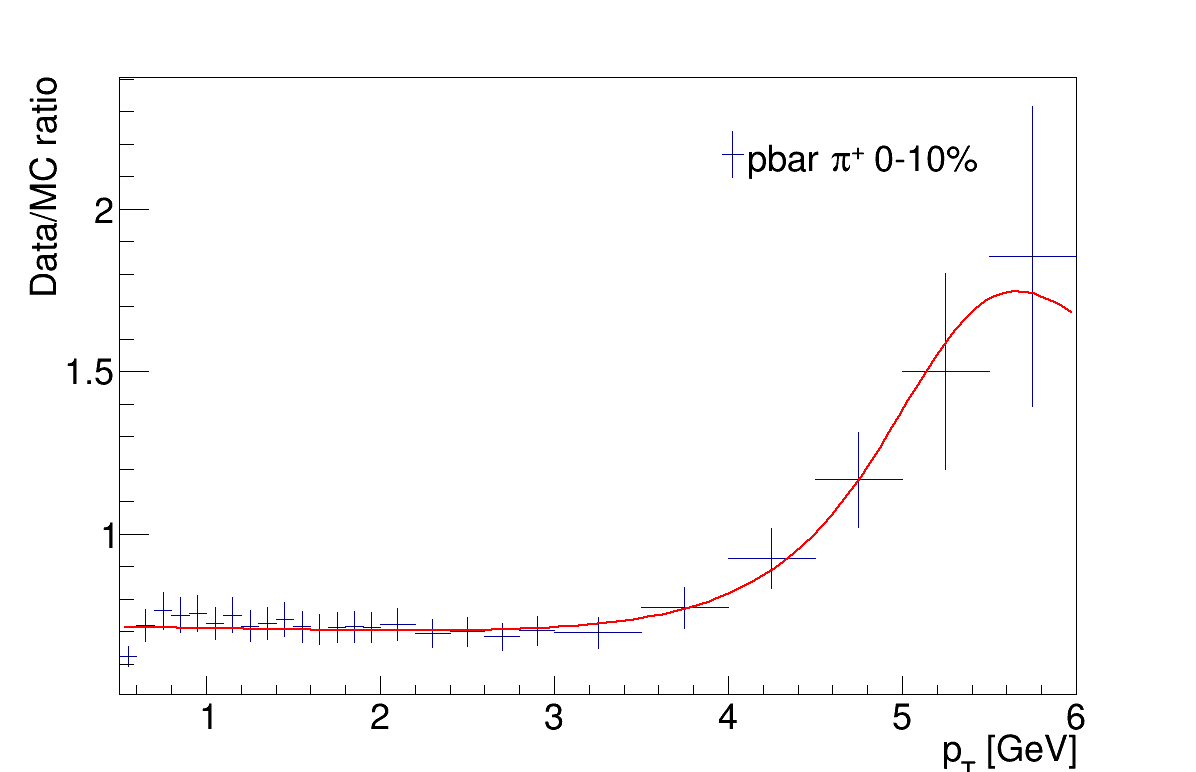
\includegraphics[width=0.24\linewidth]{detdeta/Figures/particle_reweighting_ratios/EPOS_pbar_0.png}
    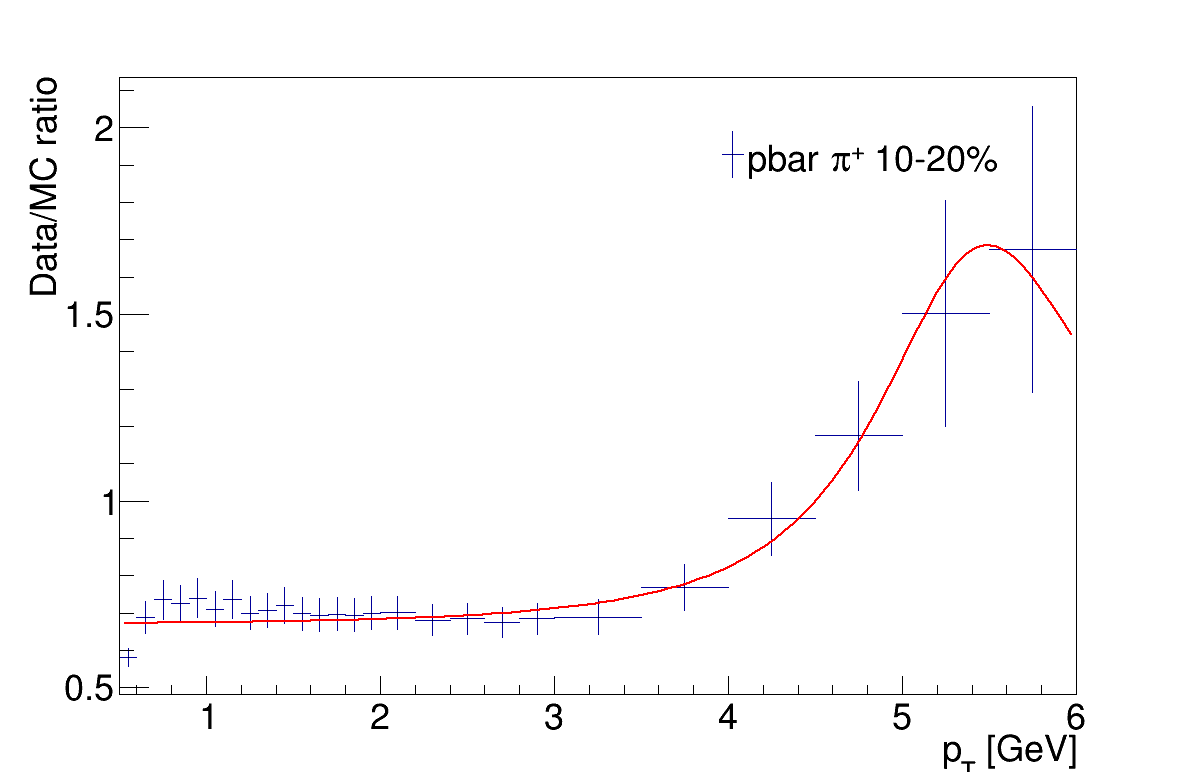
\includegraphics[width=0.24\linewidth]{detdeta/Figures/particle_reweighting_ratios/EPOS_pbar_1.png}
    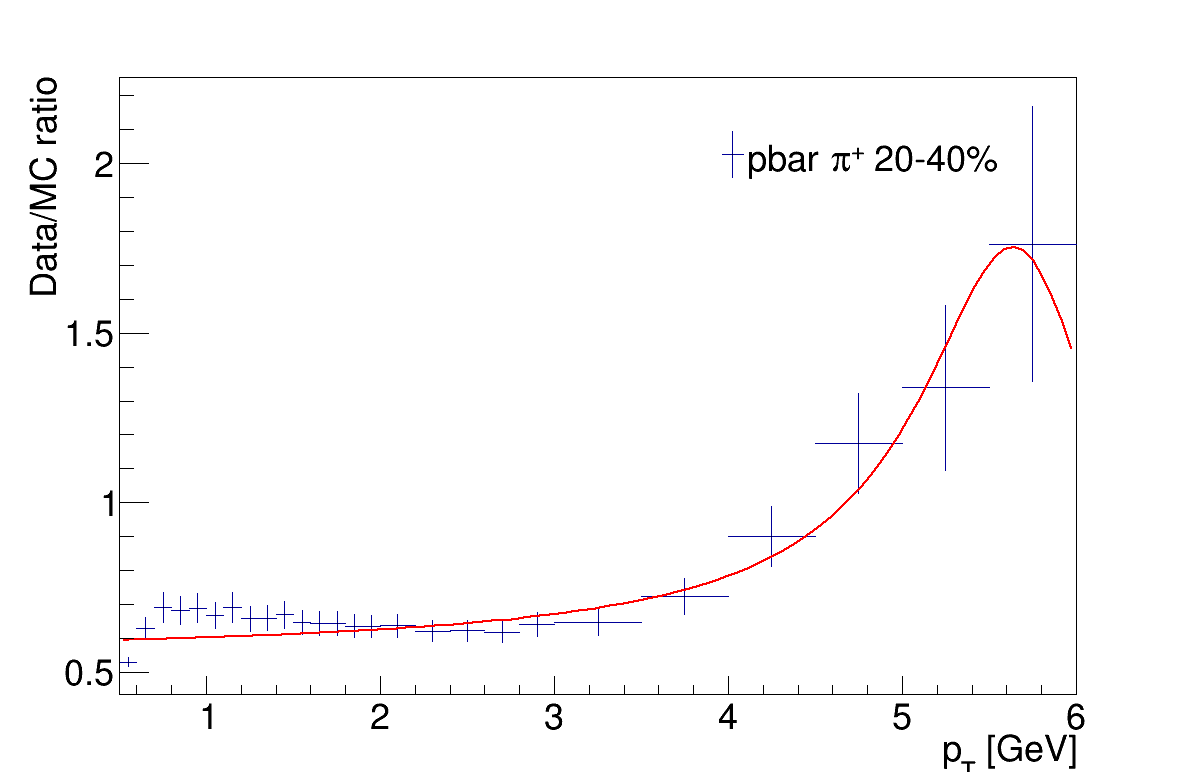
\includegraphics[width=0.24\linewidth]{detdeta/Figures/particle_reweighting_ratios/EPOS_pbar_2.png}
    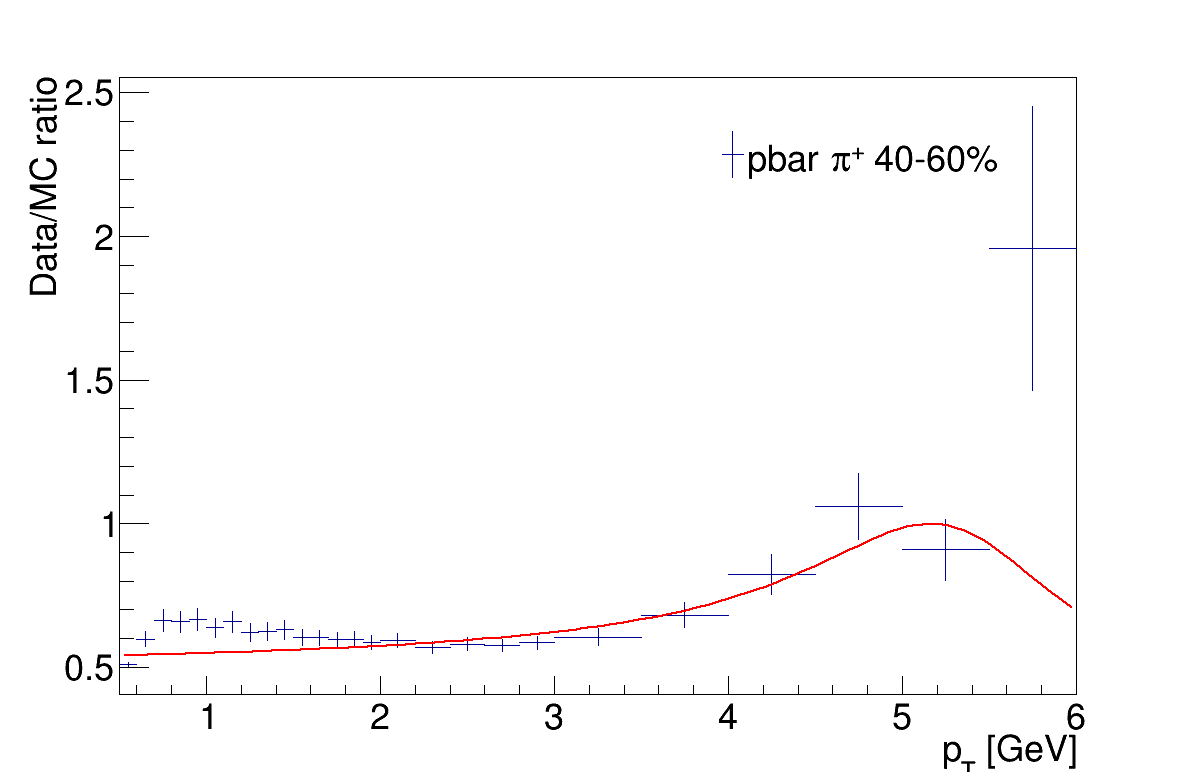
\includegraphics[width=0.24\linewidth]{detdeta/Figures/particle_reweighting_ratios/EPOS_pbar_3.png}
    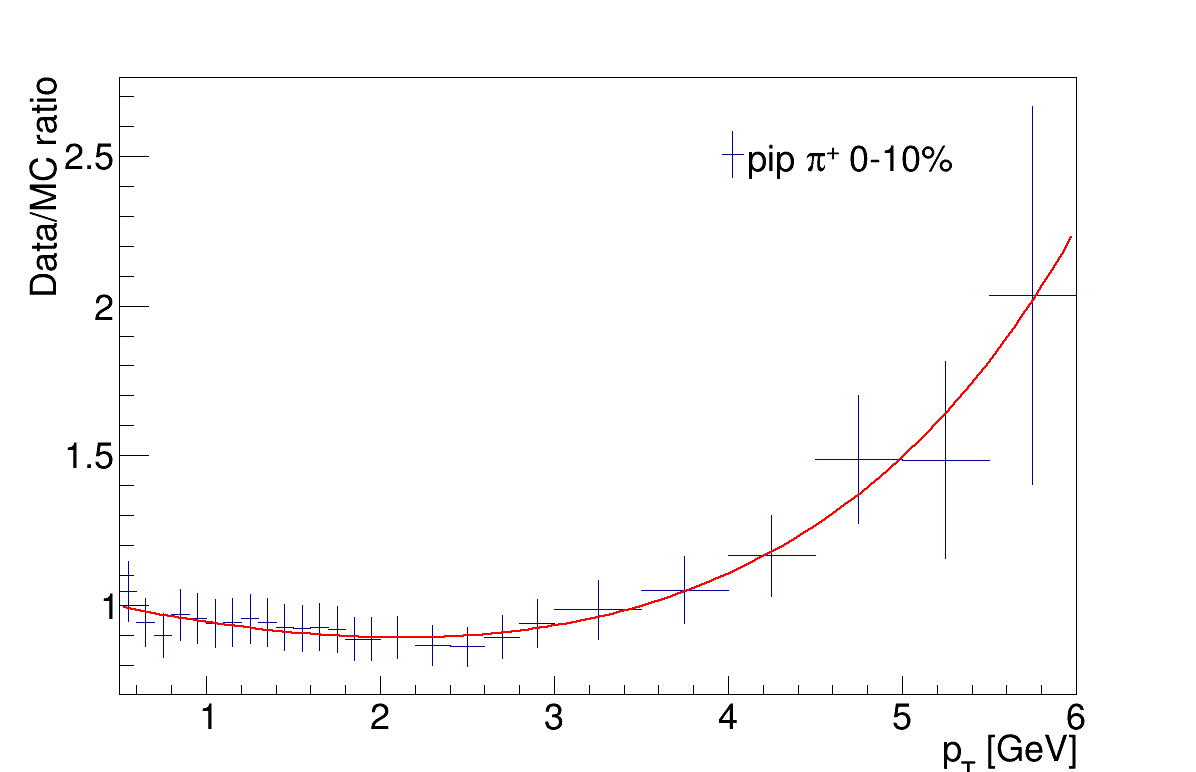
\includegraphics[width=0.24\linewidth]{detdeta/Figures/particle_reweighting_ratios/EPOS_pip_0.png}
    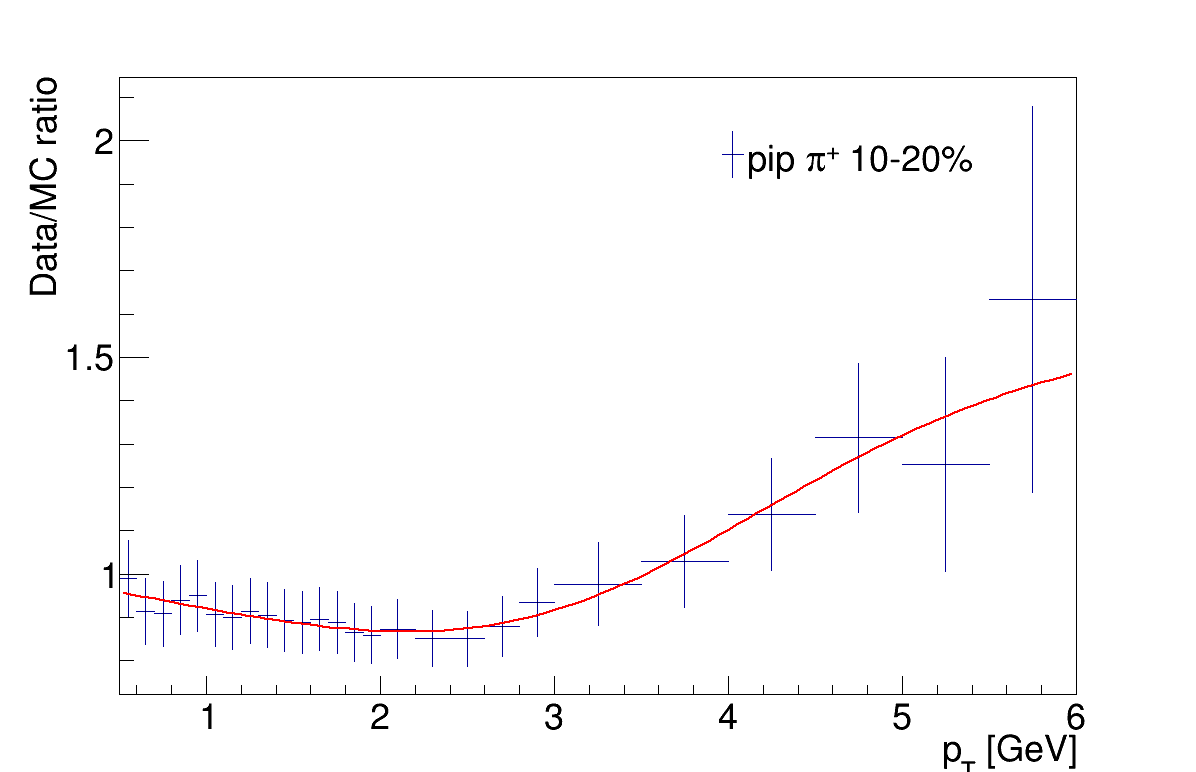
\includegraphics[width=0.24\linewidth]{detdeta/Figures/particle_reweighting_ratios/EPOS_pip_1.png}
    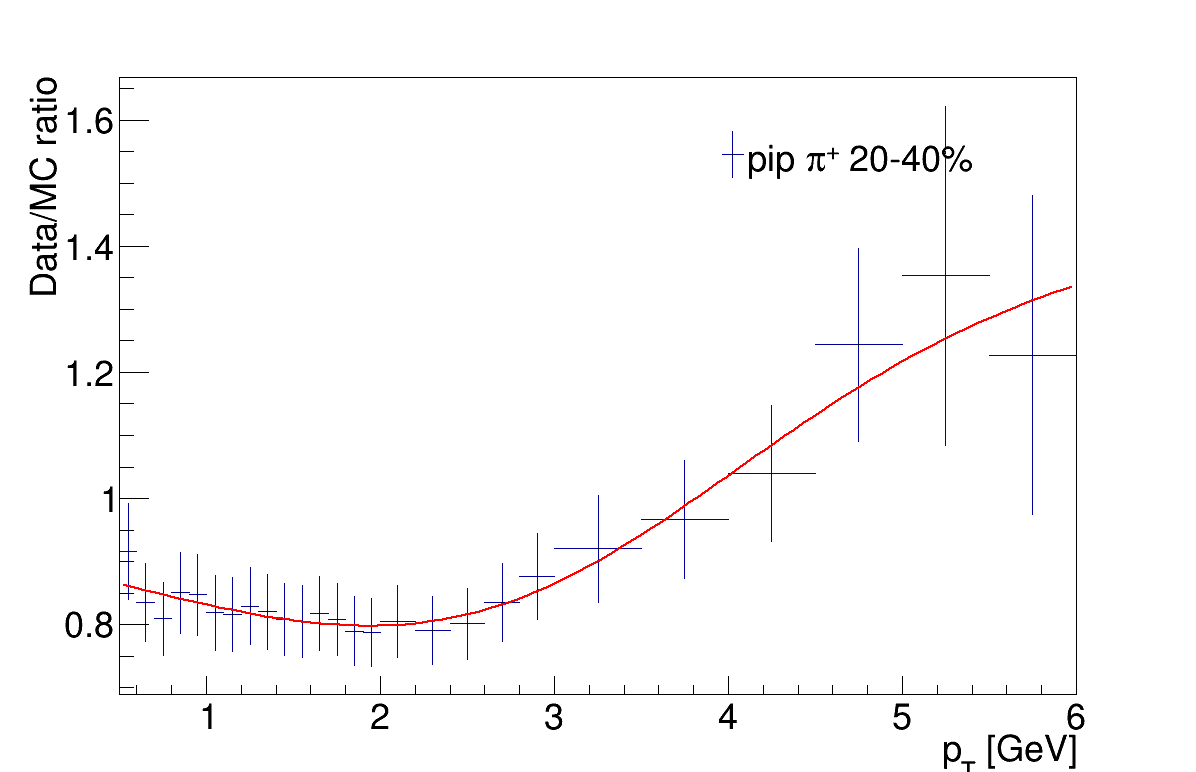
\includegraphics[width=0.24\linewidth]{detdeta/Figures/particle_reweighting_ratios/EPOS_pip_2.png}
    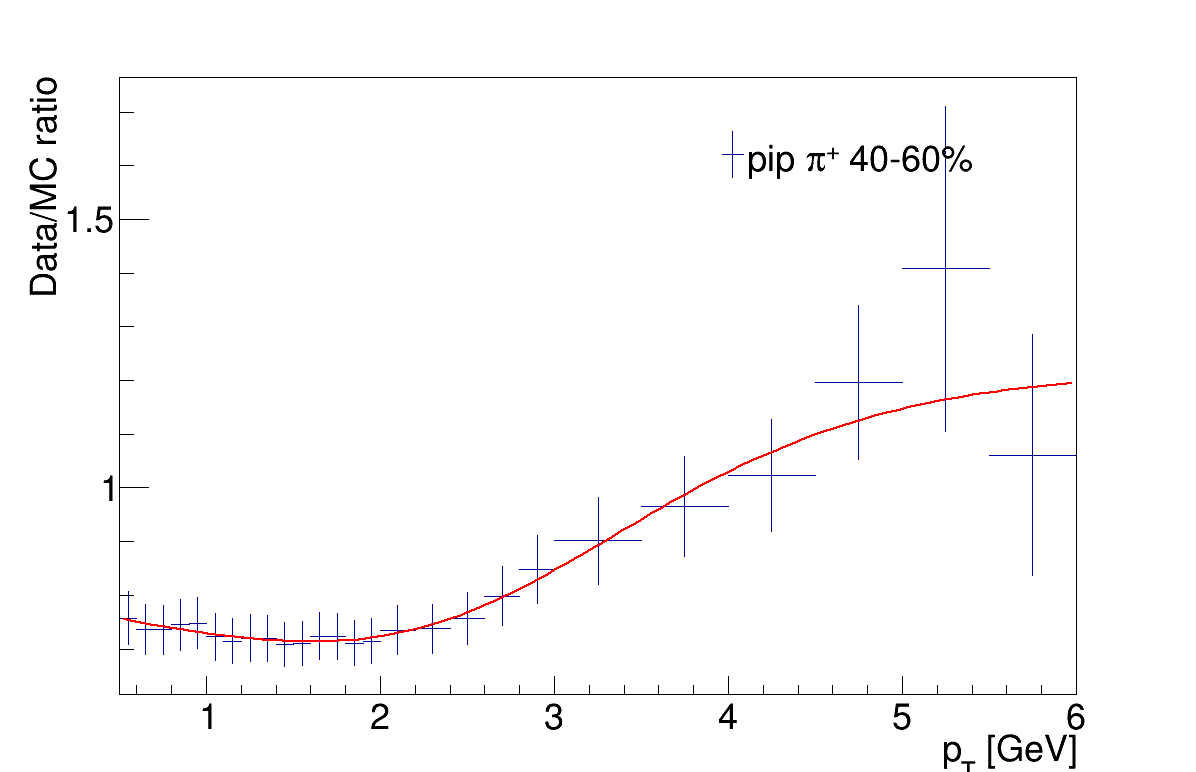
\includegraphics[width=0.24\linewidth]{detdeta/Figures/particle_reweighting_ratios/EPOS_pip_3.png}
    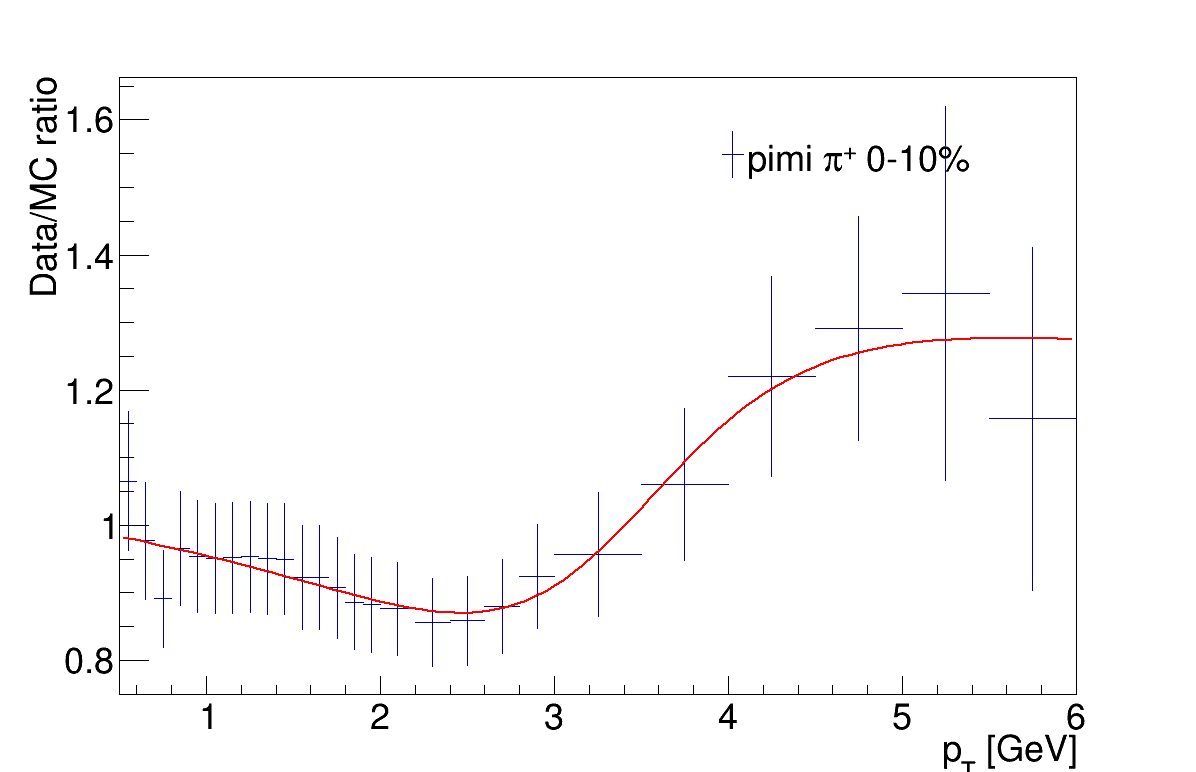
\includegraphics[width=0.24\linewidth]{detdeta/Figures/particle_reweighting_ratios/EPOS_pimi_0.png}
    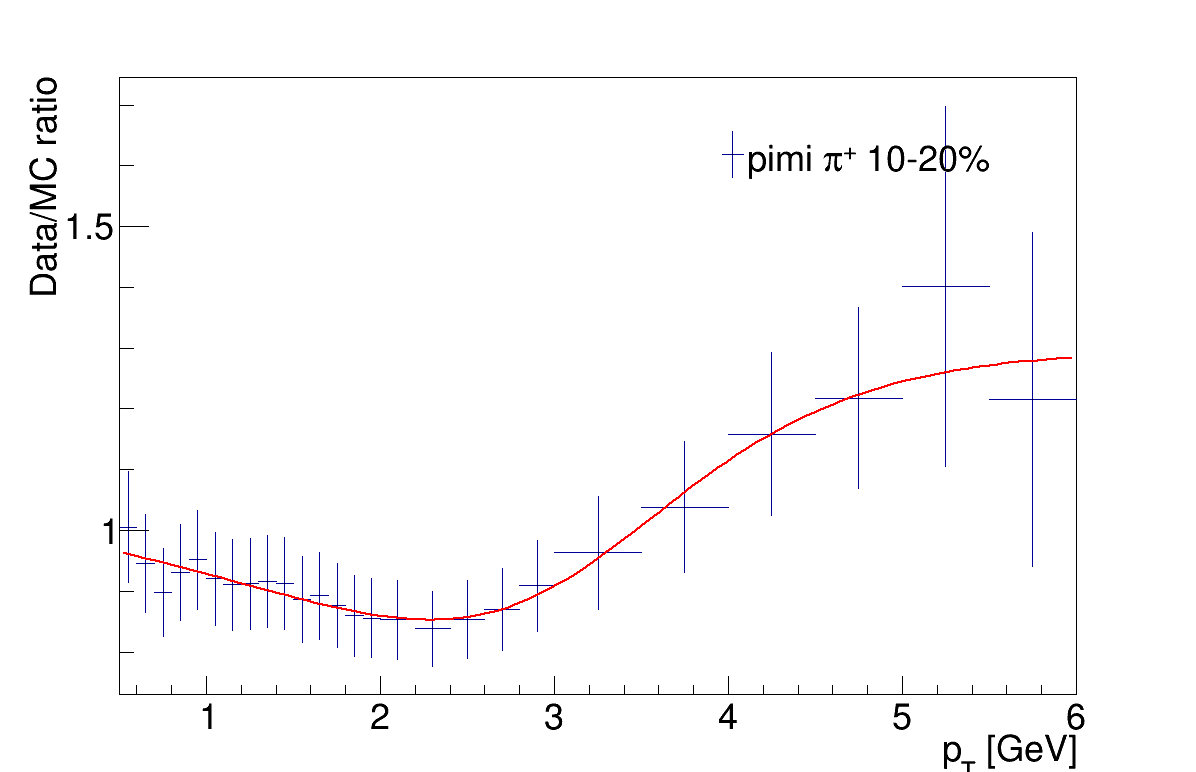
\includegraphics[width=0.24\linewidth]{detdeta/Figures/particle_reweighting_ratios/EPOS_pimi_1.png}
    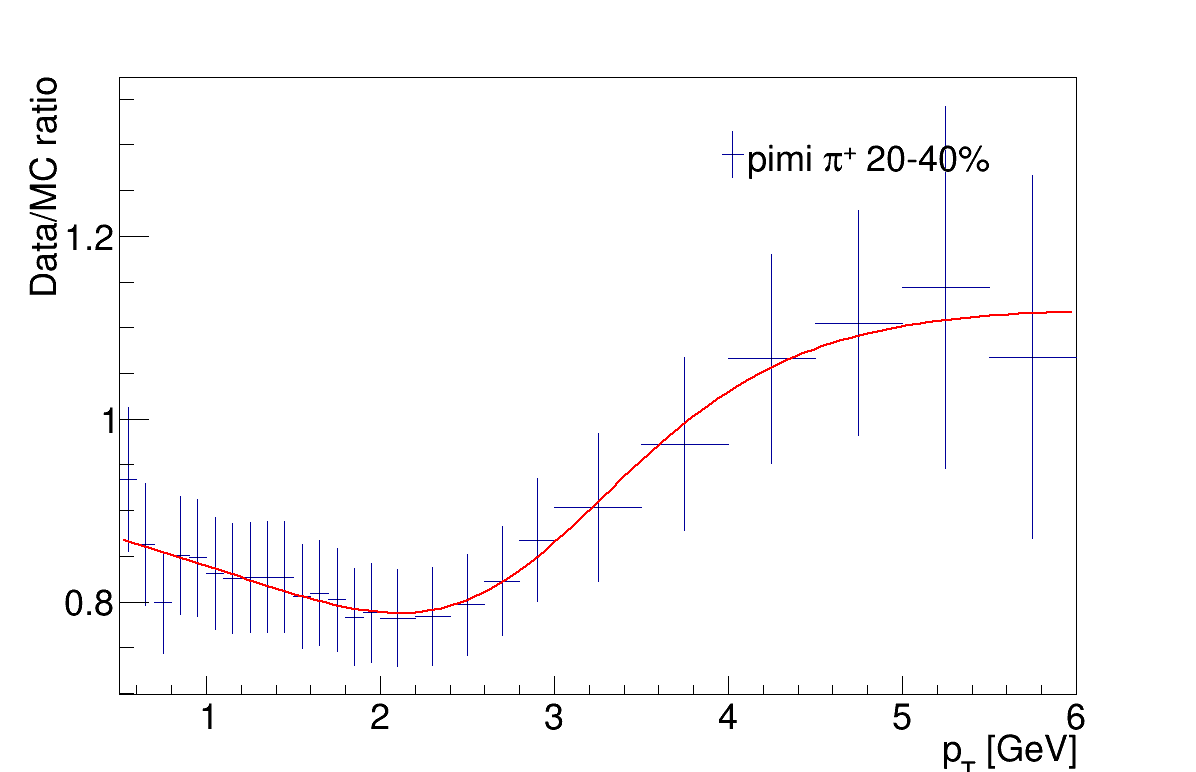
\includegraphics[width=0.24\linewidth]{detdeta/Figures/particle_reweighting_ratios/EPOS_pimi_2.png}
    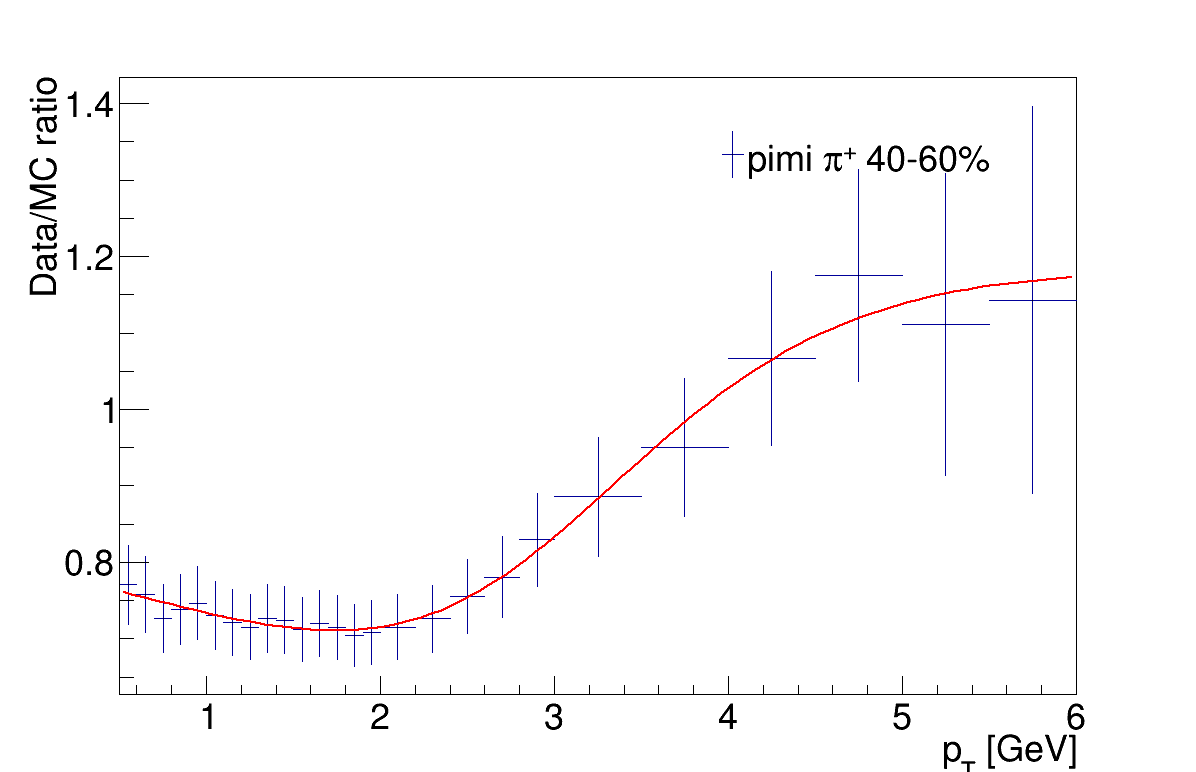
\includegraphics[width=0.24\linewidth]{detdeta/Figures/particle_reweighting_ratios/EPOS_pimi_3.png}
    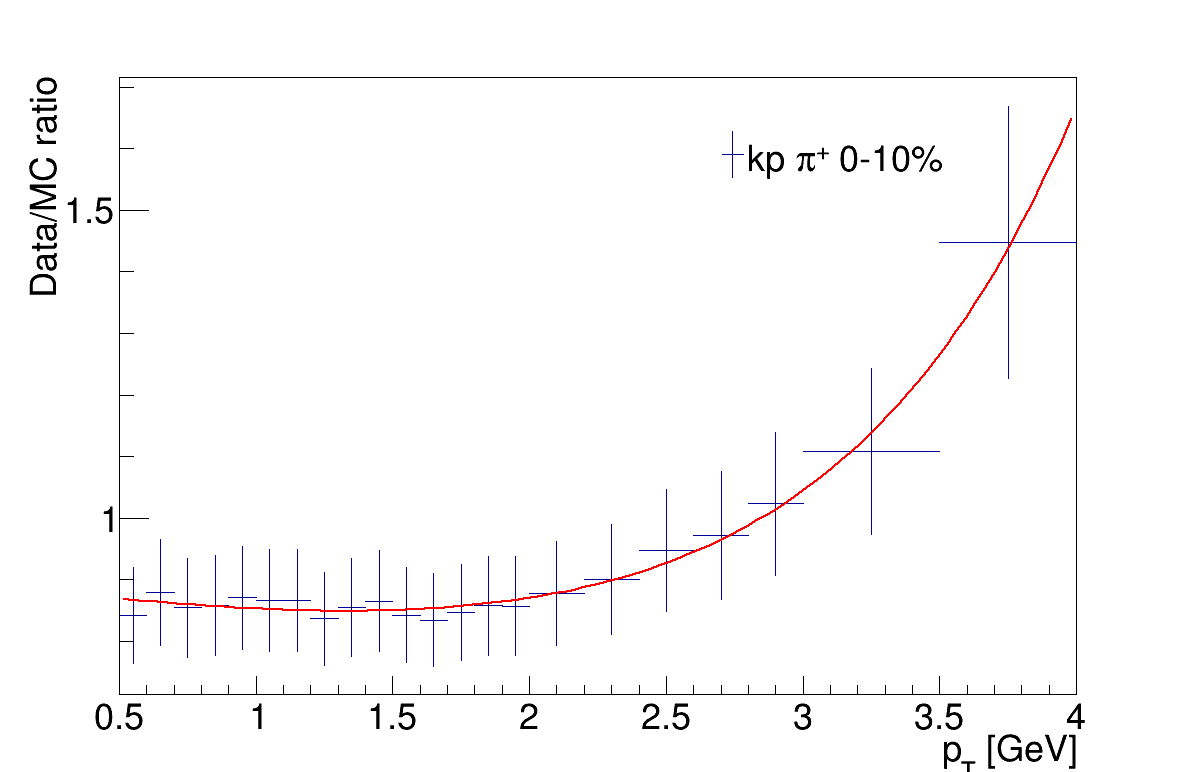
\includegraphics[width=0.24\linewidth]{detdeta/Figures/particle_reweighting_ratios/EPOS_kp_0.png}
    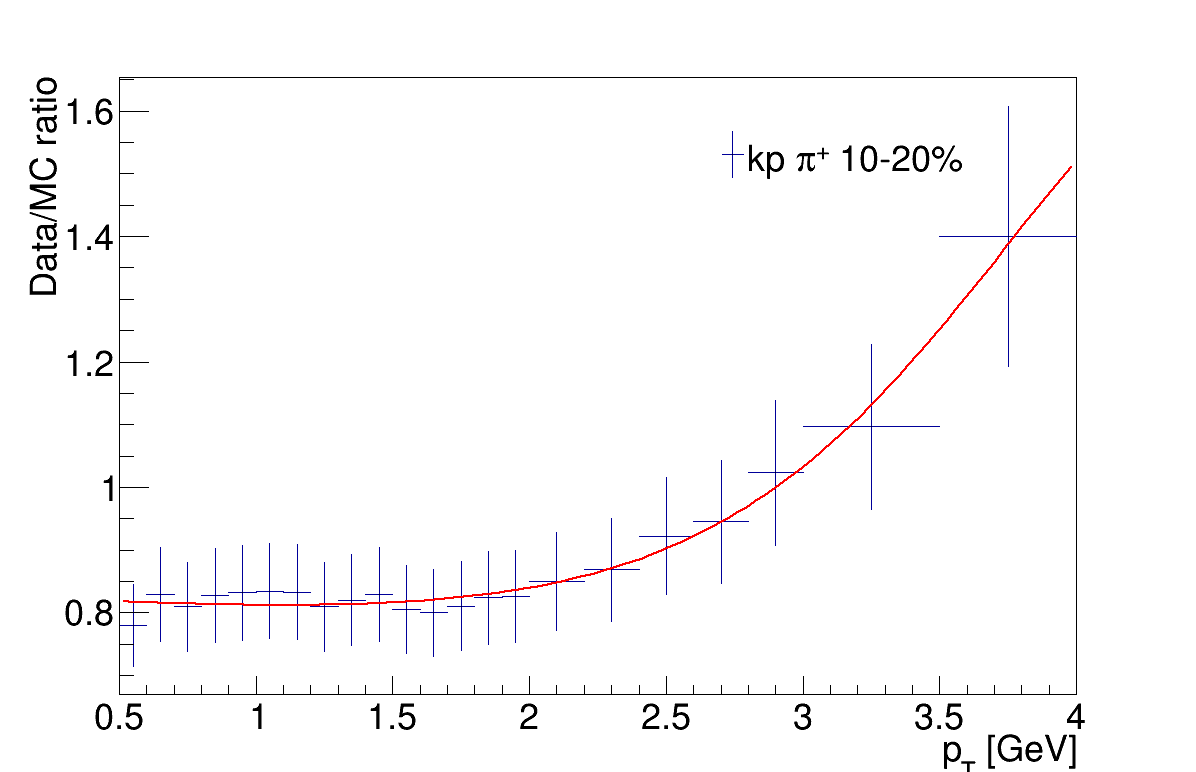
\includegraphics[width=0.24\linewidth]{detdeta/Figures/particle_reweighting_ratios/EPOS_kp_1.png}
    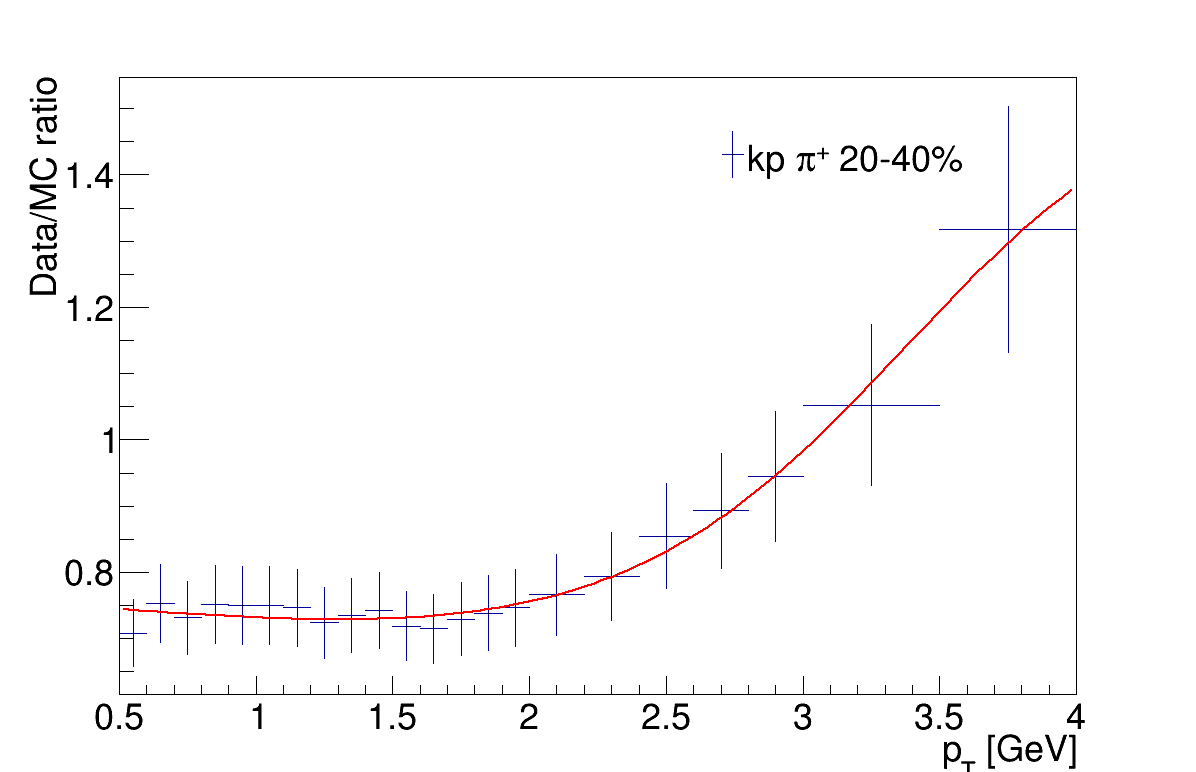
\includegraphics[width=0.24\linewidth]{detdeta/Figures/particle_reweighting_ratios/EPOS_kp_2.png}
    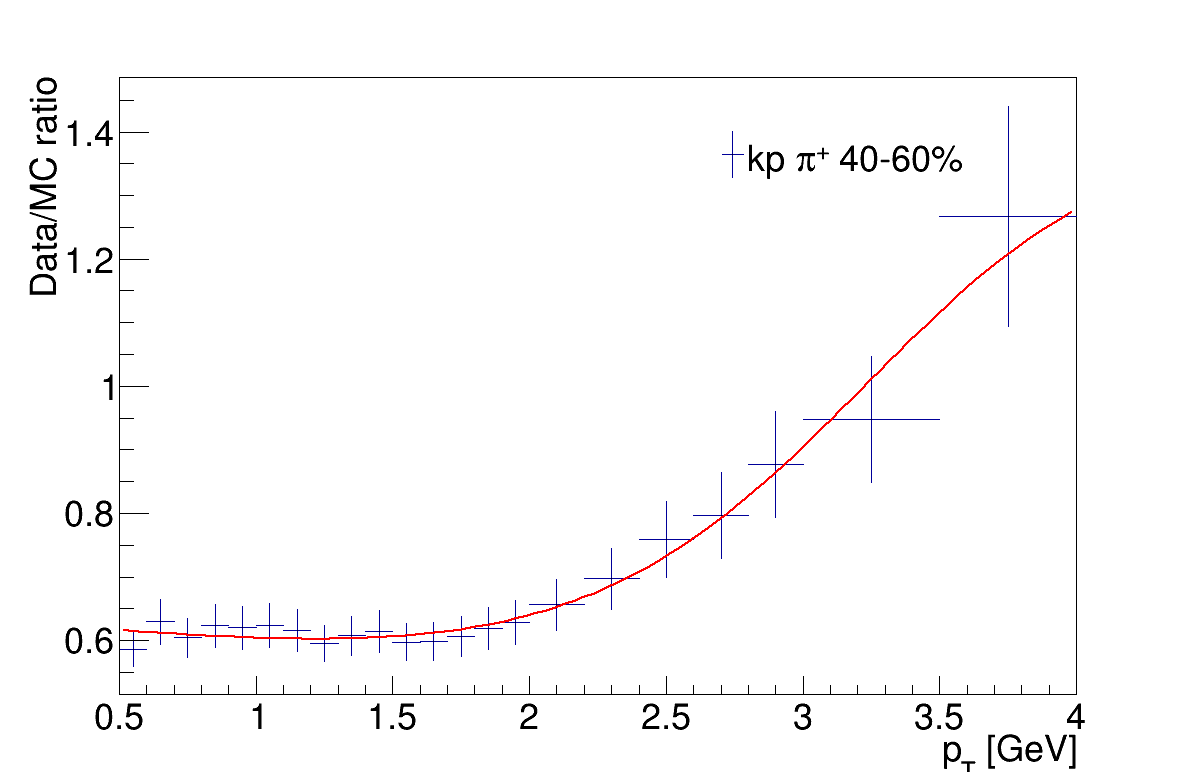
\includegraphics[width=0.24\linewidth]{detdeta/Figures/particle_reweighting_ratios/EPOS_kp_3.png}
    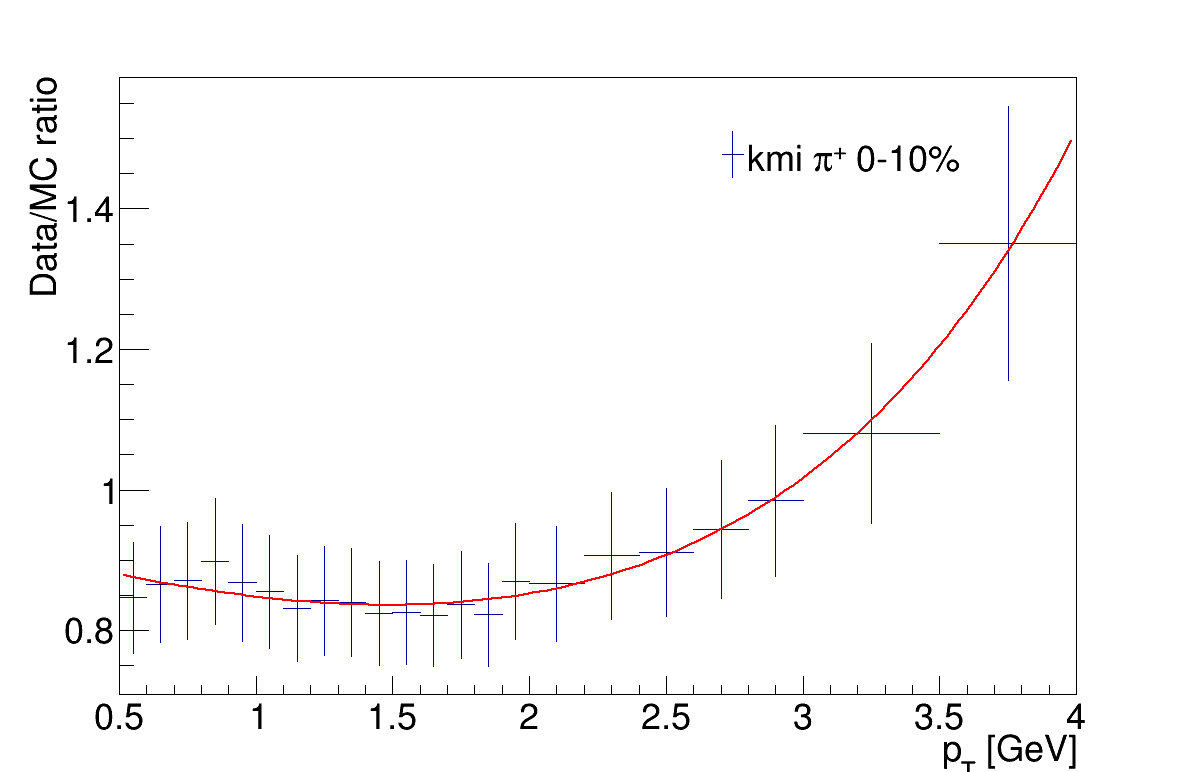
\includegraphics[width=0.24\linewidth]{detdeta/Figures/particle_reweighting_ratios/EPOS_kmi_0.png}
    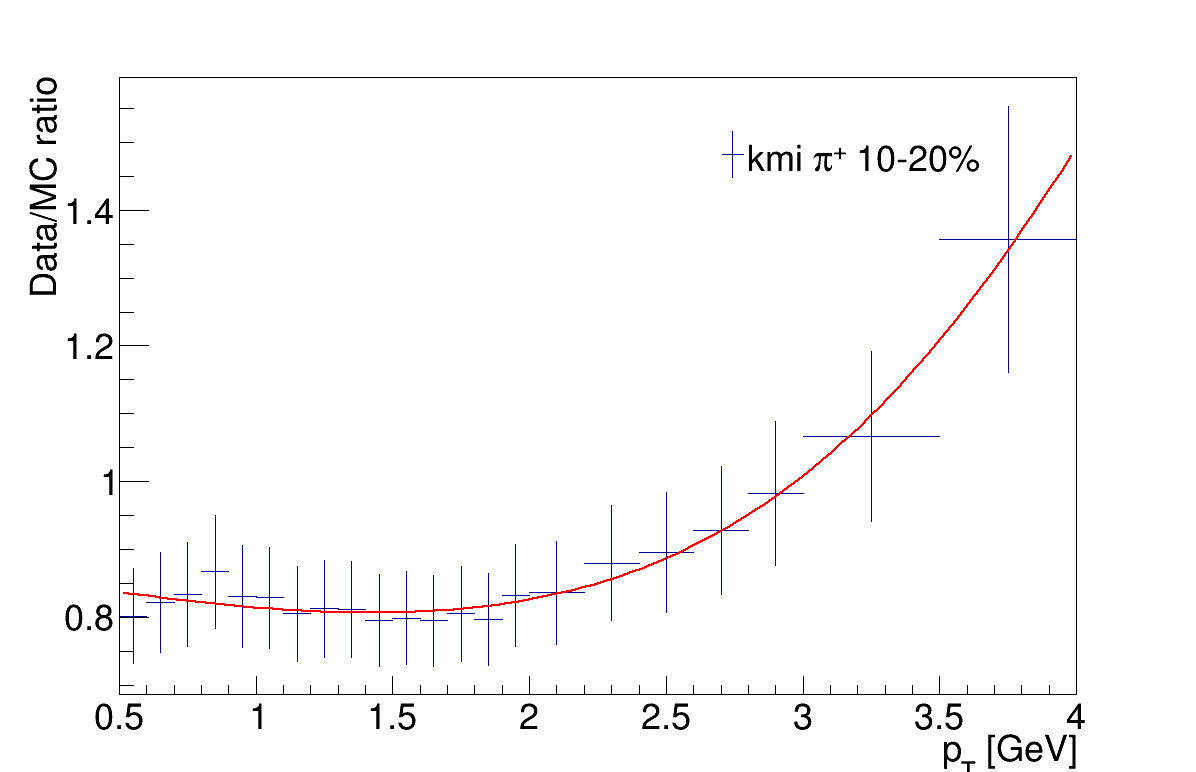
\includegraphics[width=0.24\linewidth]{detdeta/Figures/particle_reweighting_ratios/EPOS_kmi_1.png}
    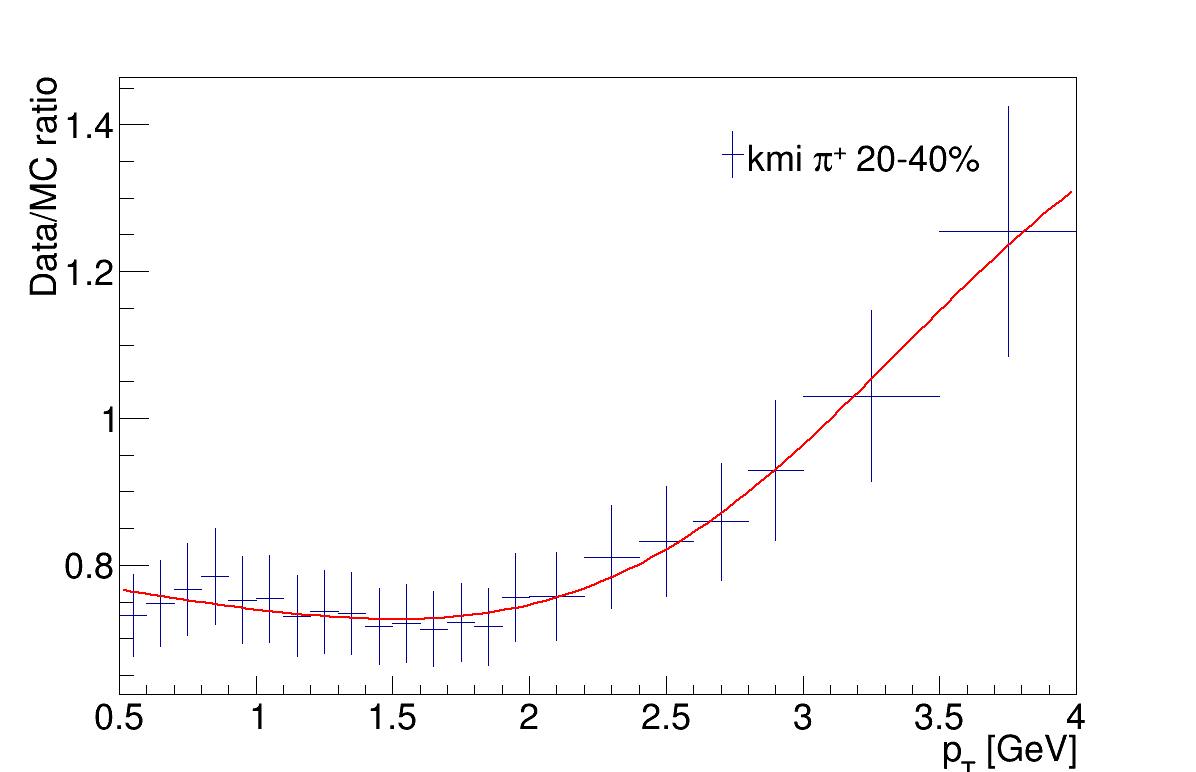
\includegraphics[width=0.24\linewidth]{detdeta/Figures/particle_reweighting_ratios/EPOS_kmi_2.png}
    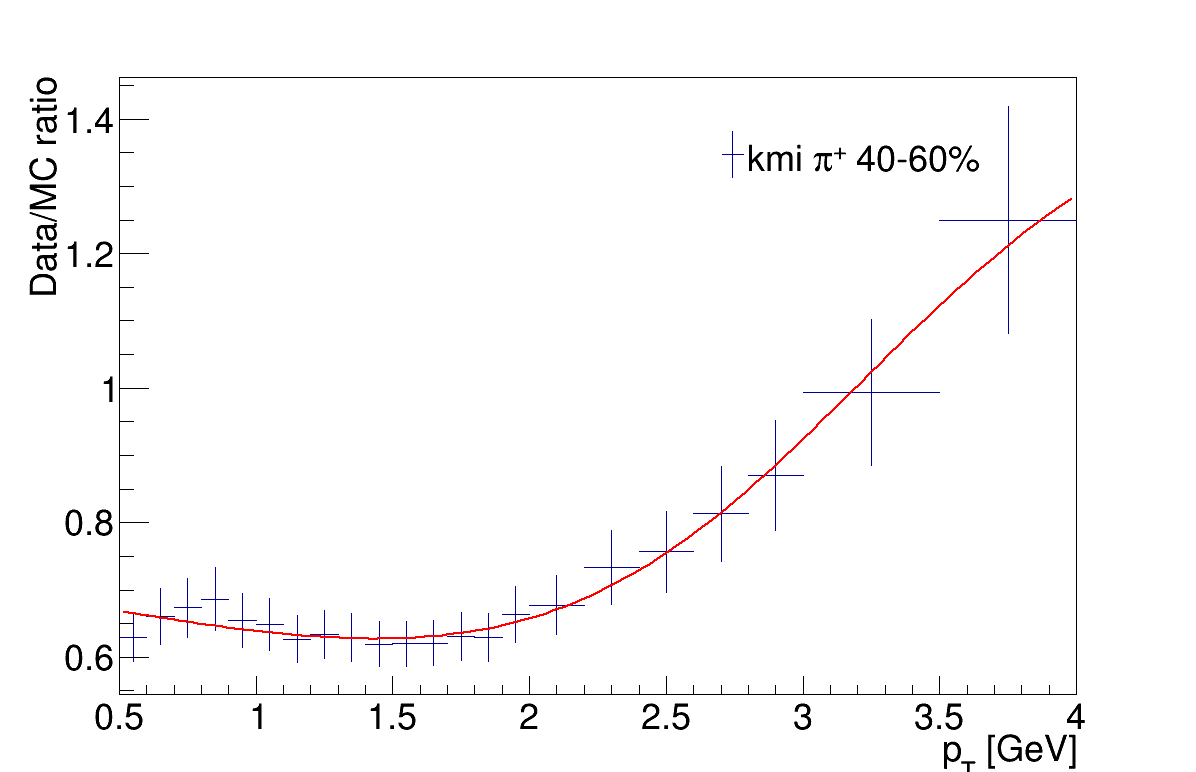
\includegraphics[width=0.24\linewidth]{detdeta/Figures/particle_reweighting_ratios/EPOS_kmi_3.png}
    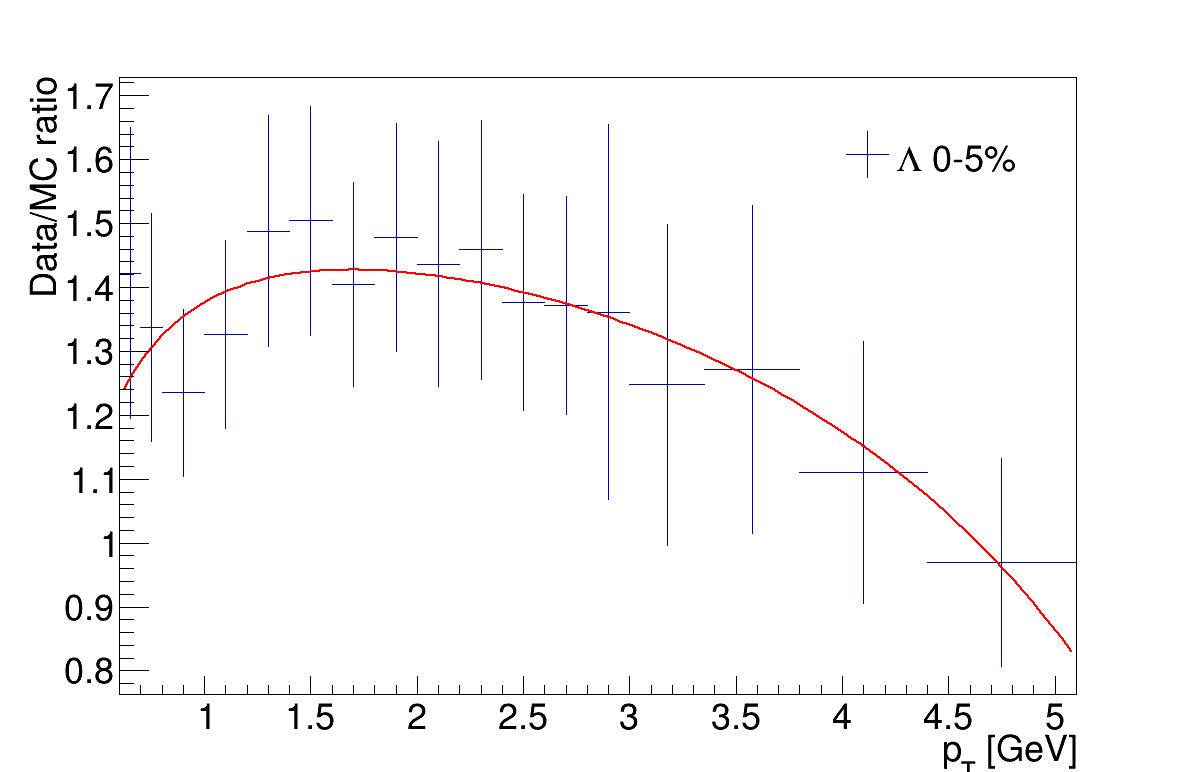
\includegraphics[width=0.24\linewidth]{detdeta/Figures/particle_reweighting_ratios/EPOS_lambda_0.png}
    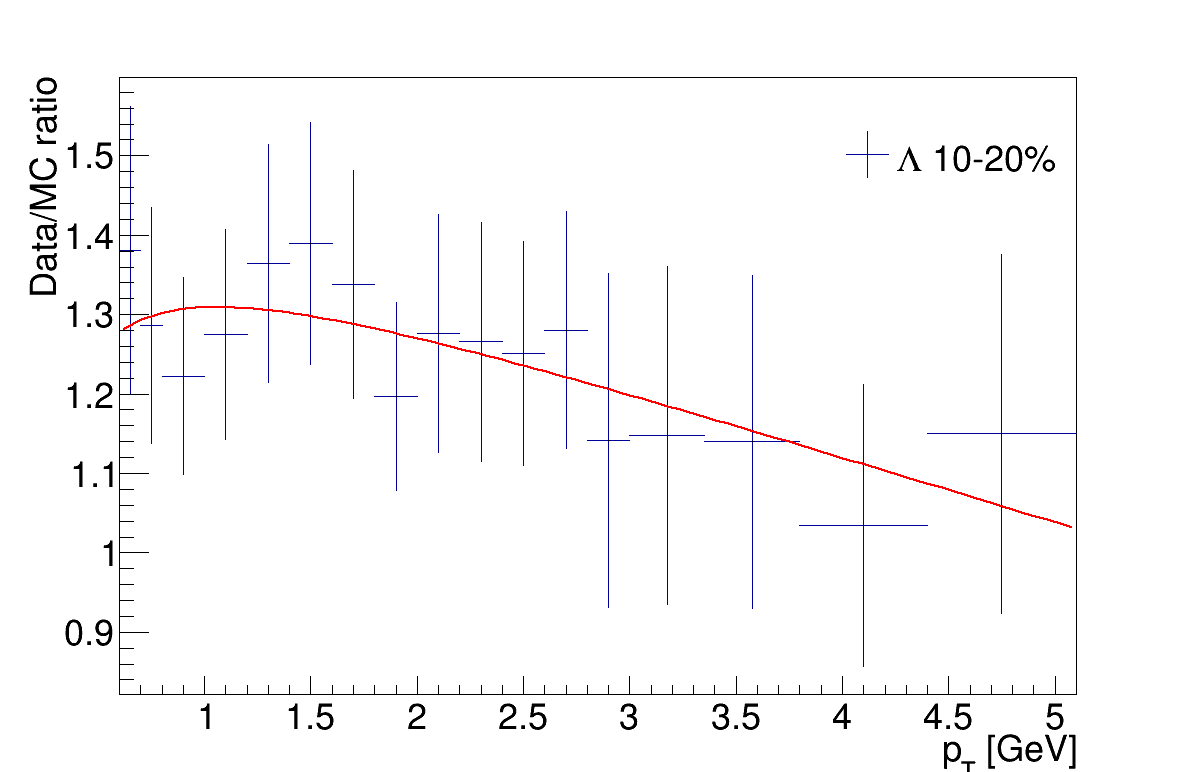
\includegraphics[width=0.24\linewidth]{detdeta/Figures/particle_reweighting_ratios/EPOS_lambda_1.png}
    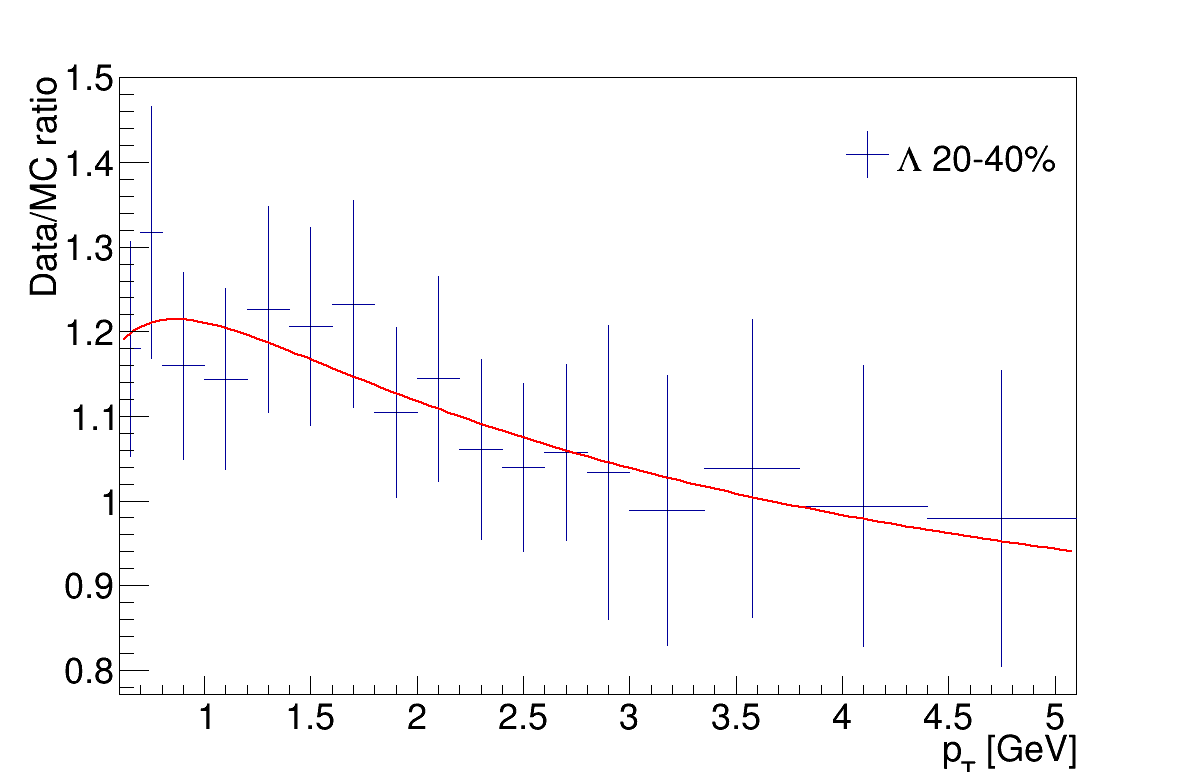
\includegraphics[width=0.24\linewidth]{detdeta/Figures/particle_reweighting_ratios/EPOS_lambda_2.png}
    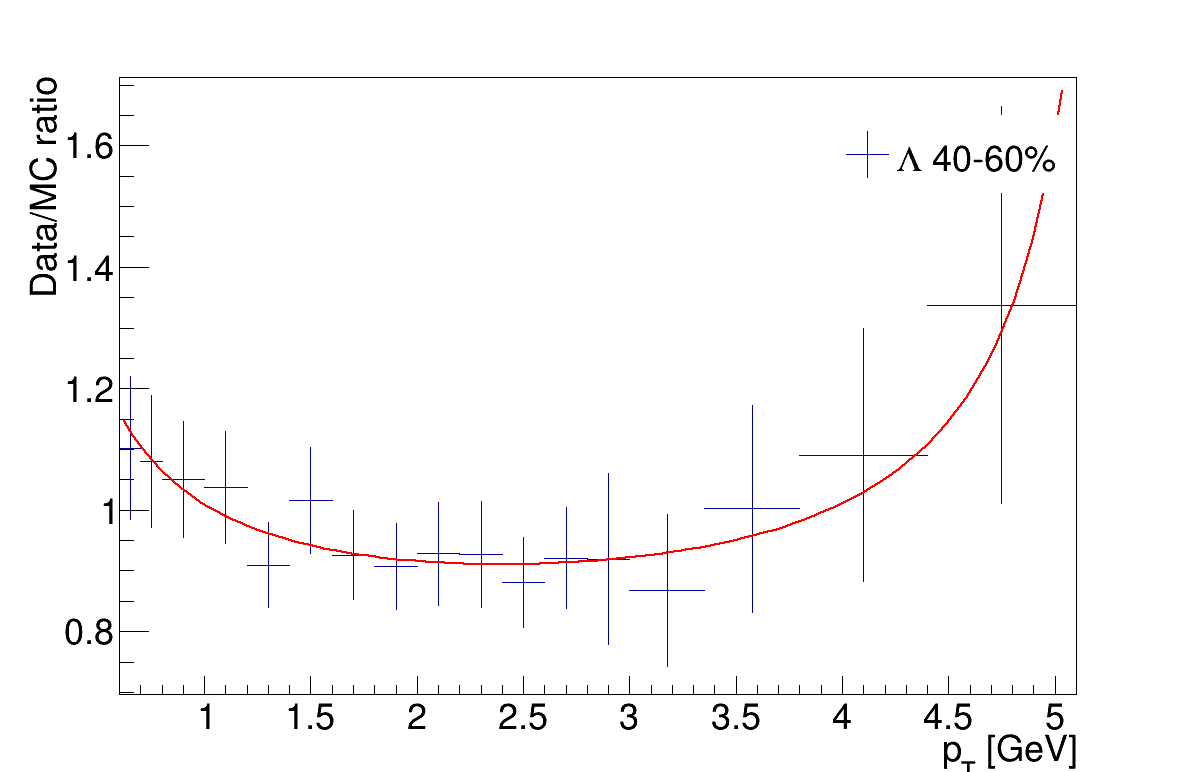
\includegraphics[width=0.24\linewidth]{detdeta/Figures/particle_reweighting_ratios/EPOS_lambda_3.png}
    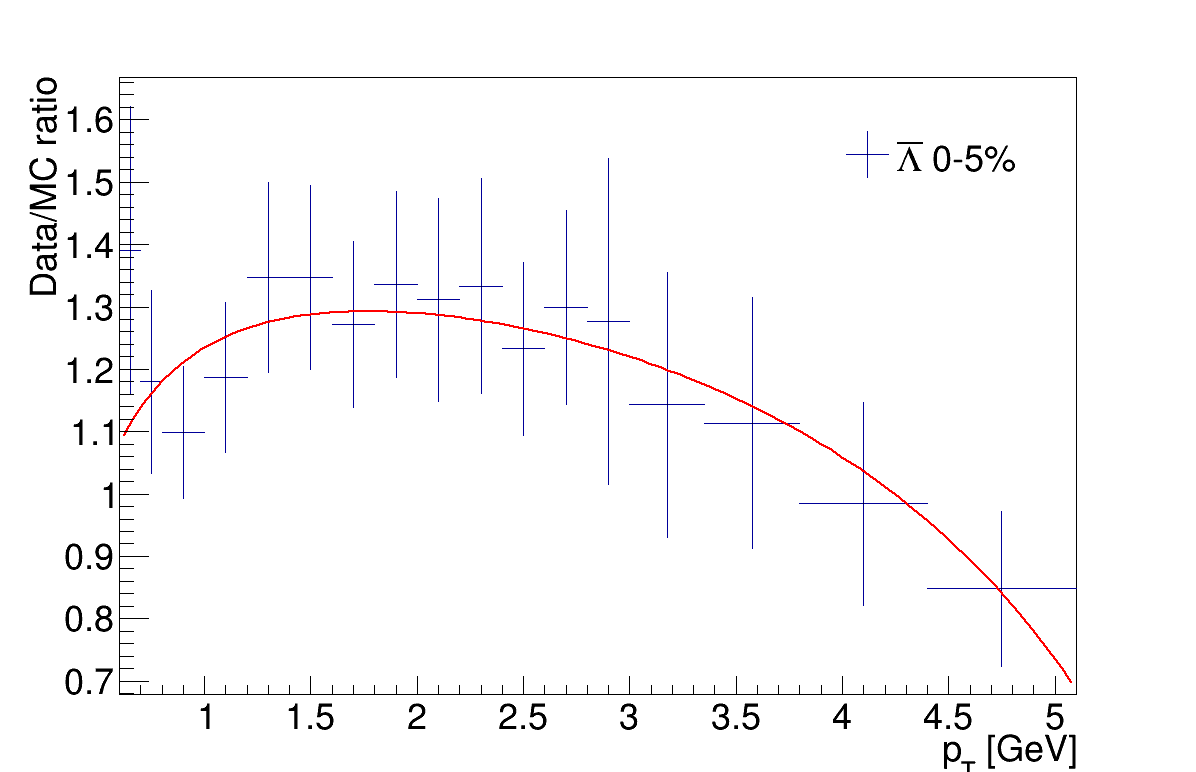
\includegraphics[width=0.24\linewidth]{detdeta/Figures/particle_reweighting_ratios/EPOS_lambda_bar_0.png}
    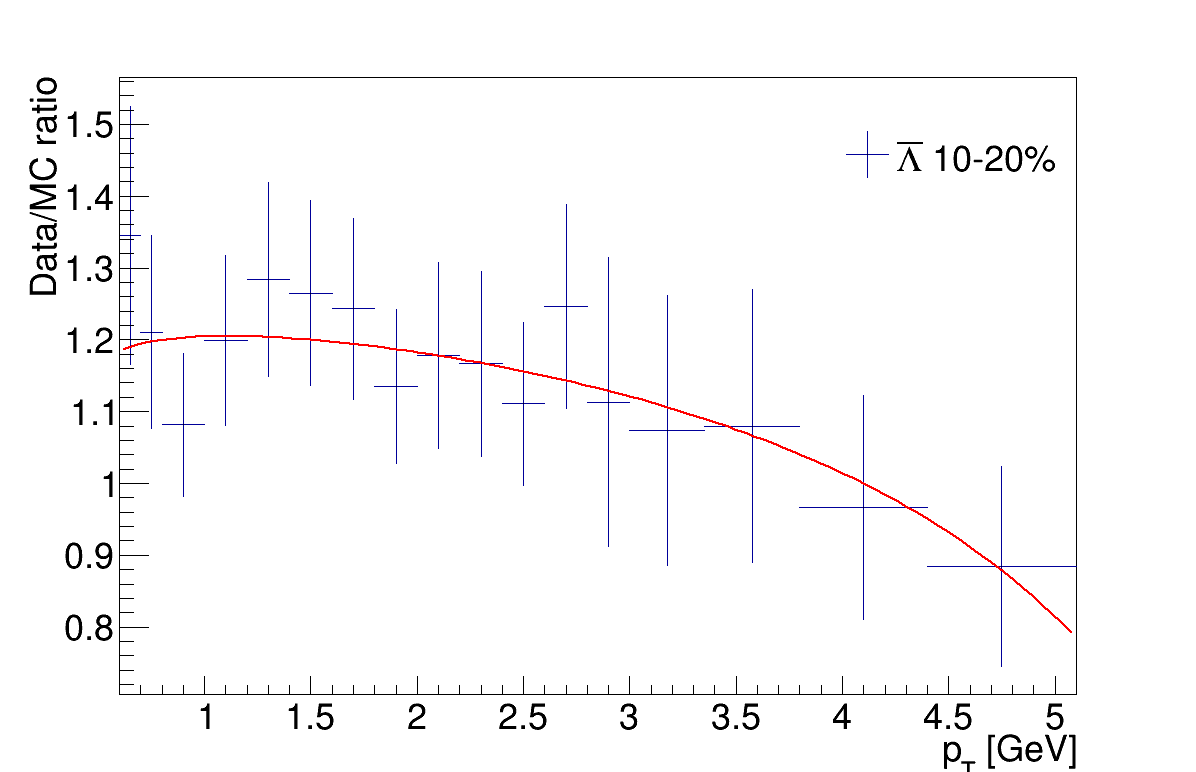
\includegraphics[width=0.24\linewidth]{detdeta/Figures/particle_reweighting_ratios/EPOS_lambda_bar_1.png}
    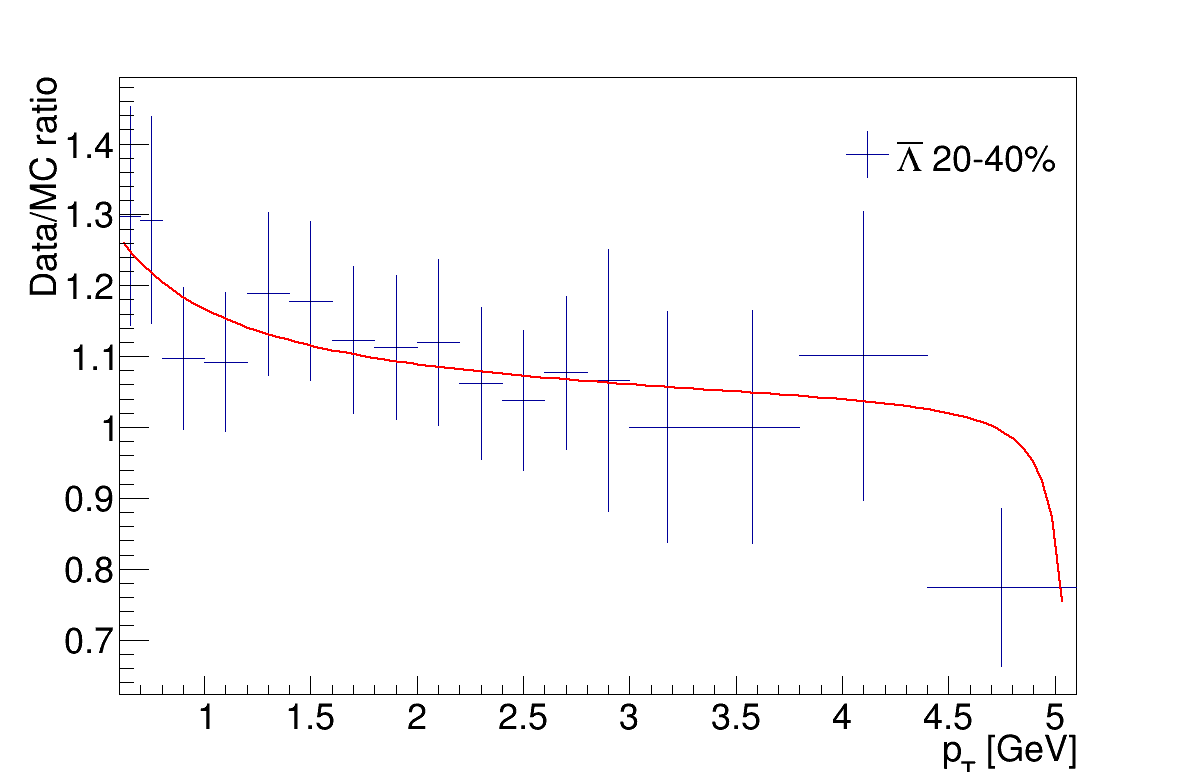
\includegraphics[width=0.24\linewidth]{detdeta/Figures/particle_reweighting_ratios/EPOS_lambda_bar_2.png}
    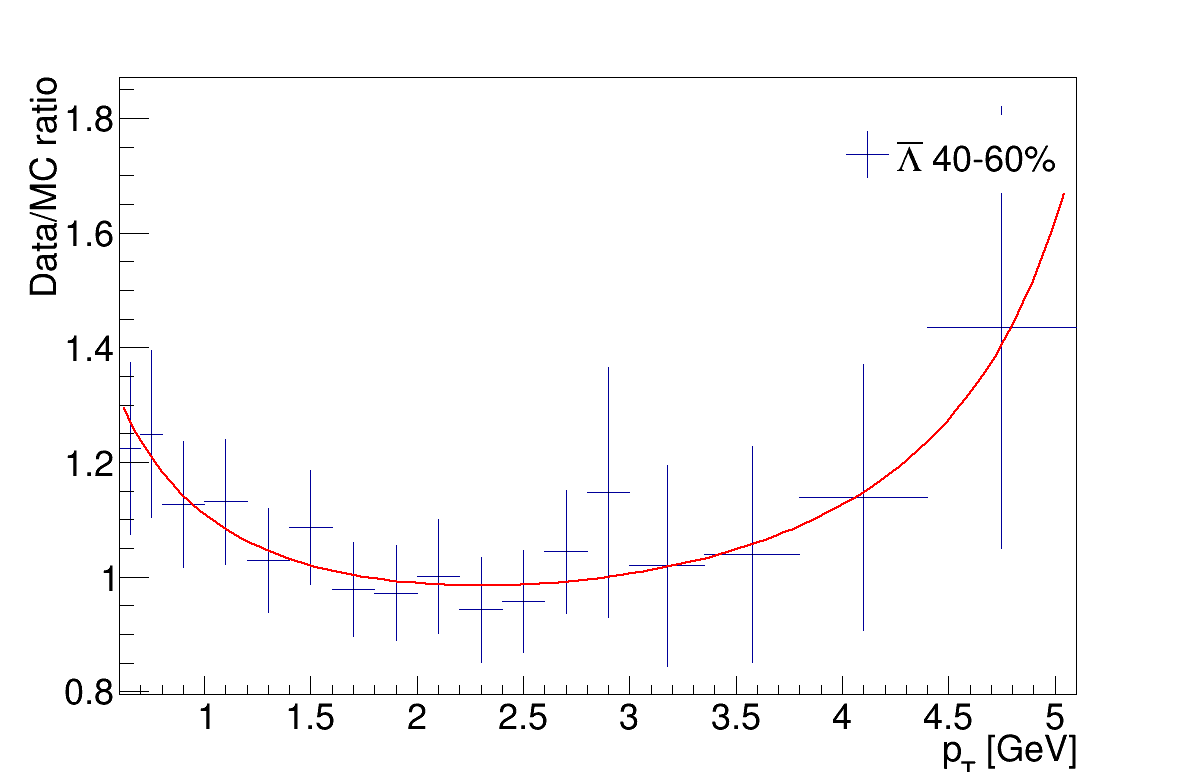
\includegraphics[width=0.24\linewidth]{detdeta/Figures/particle_reweighting_ratios/EPOS_lambda_bar_3.png}
    \caption{All data to MC ratios used in nominal EPOS reweighting method for protons, anti-protons, kaons, pions and lambda particles.}
    \label{fig:epos_data_mc_particle_ratios}
\end{figure}

\begin{figure}
    \centering
    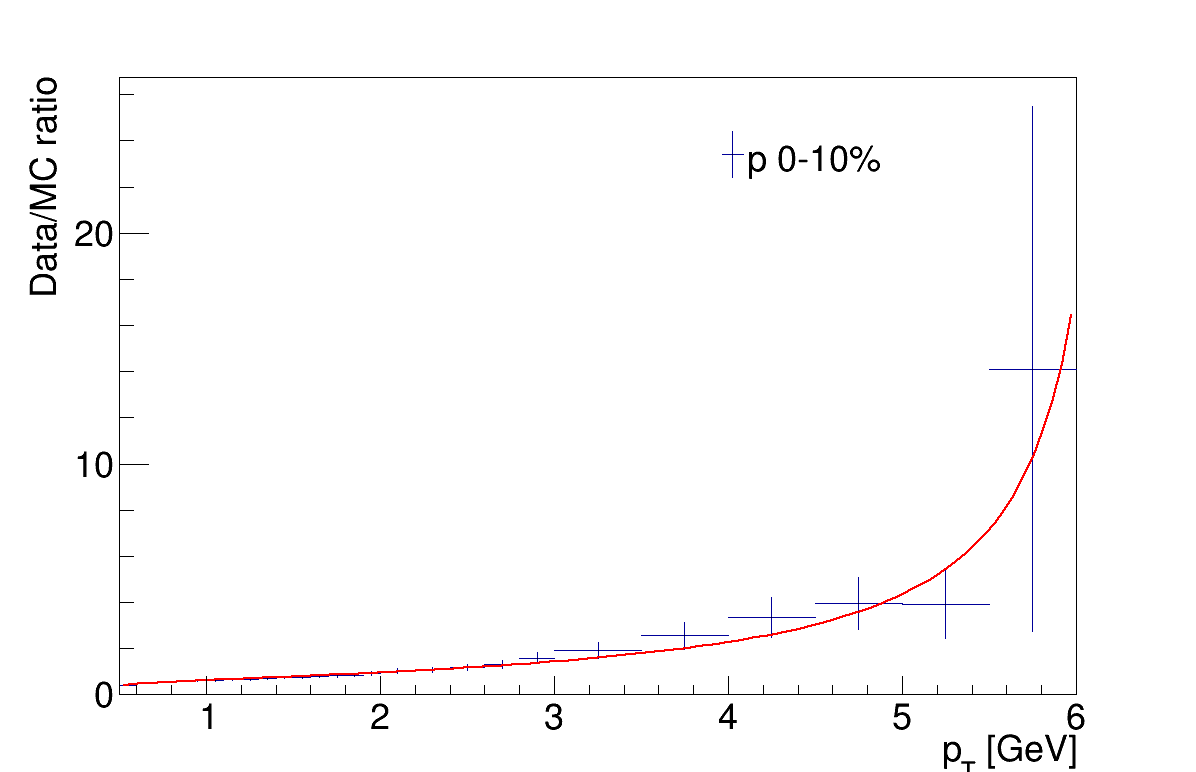
\includegraphics[width=0.24\linewidth]{detdeta/Figures/particle_reweighting_ratios/AMPT_p_0.png}
    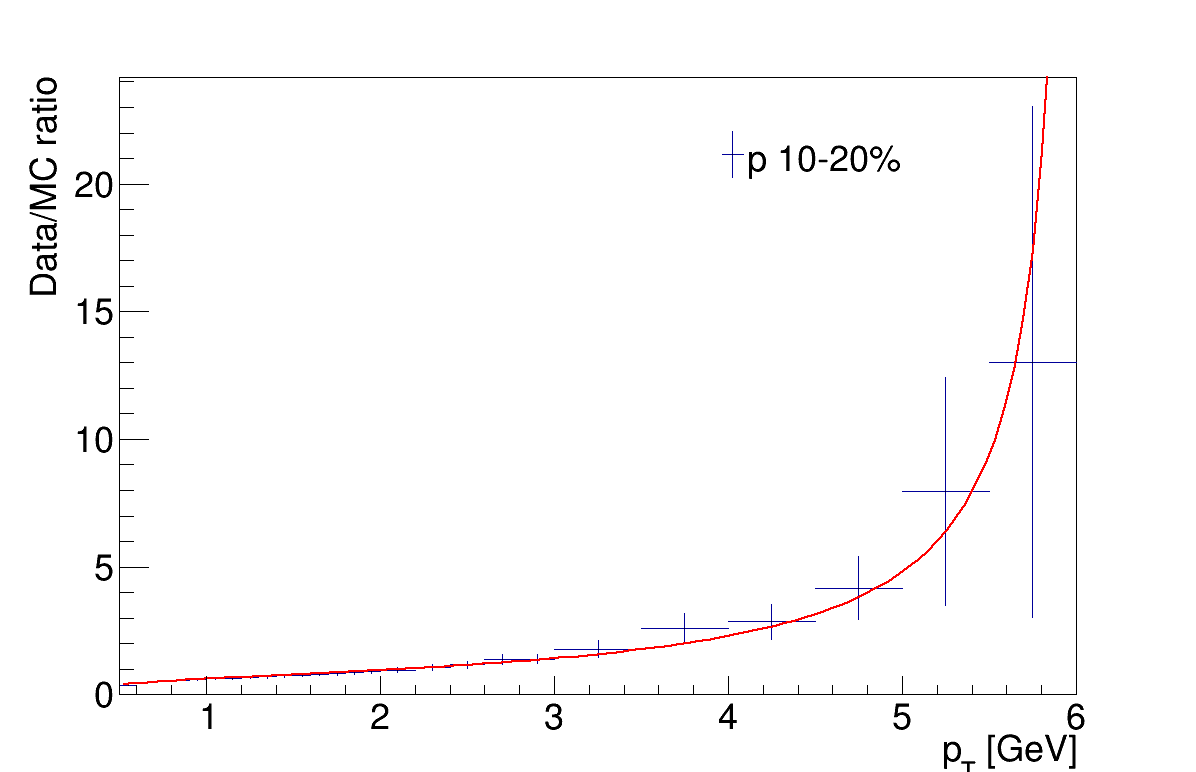
\includegraphics[width=0.24\linewidth]{detdeta/Figures/particle_reweighting_ratios/AMPT_p_1.png}
    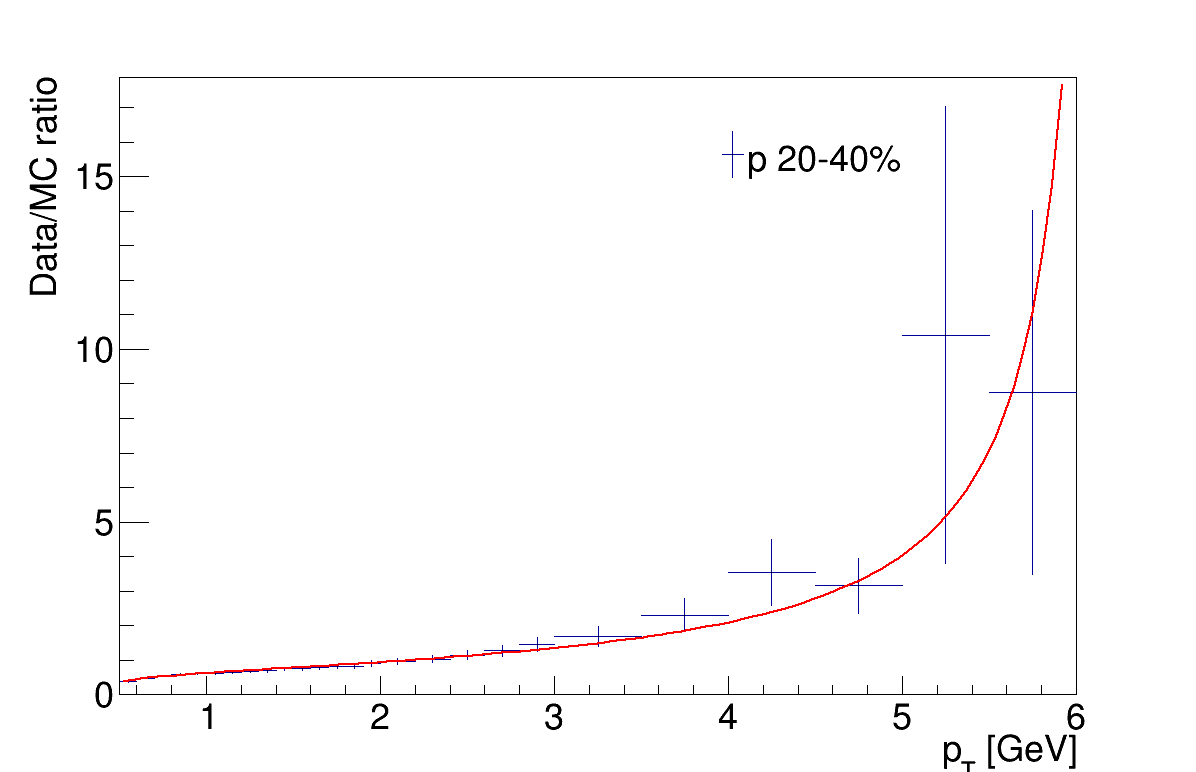
\includegraphics[width=0.24\linewidth]{detdeta/Figures/particle_reweighting_ratios/AMPT_p_2.png}
    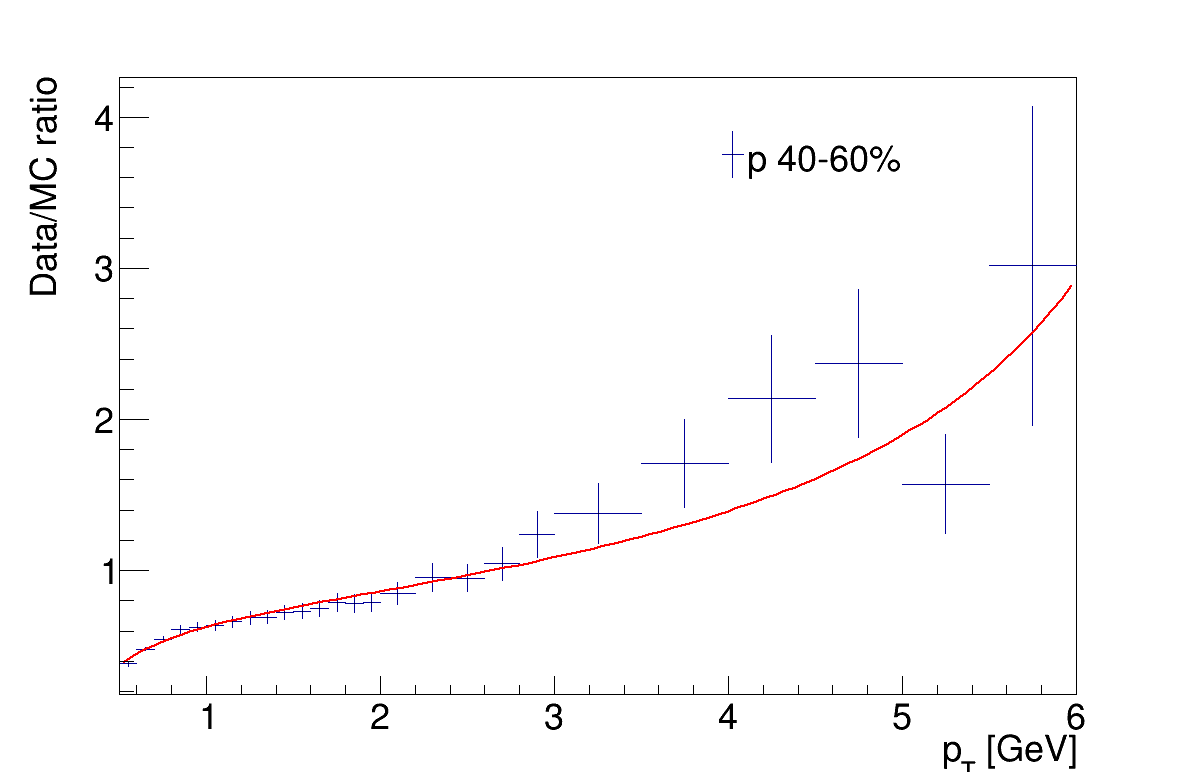
\includegraphics[width=0.24\linewidth]{detdeta/Figures/particle_reweighting_ratios/AMPT_p_3.png}
    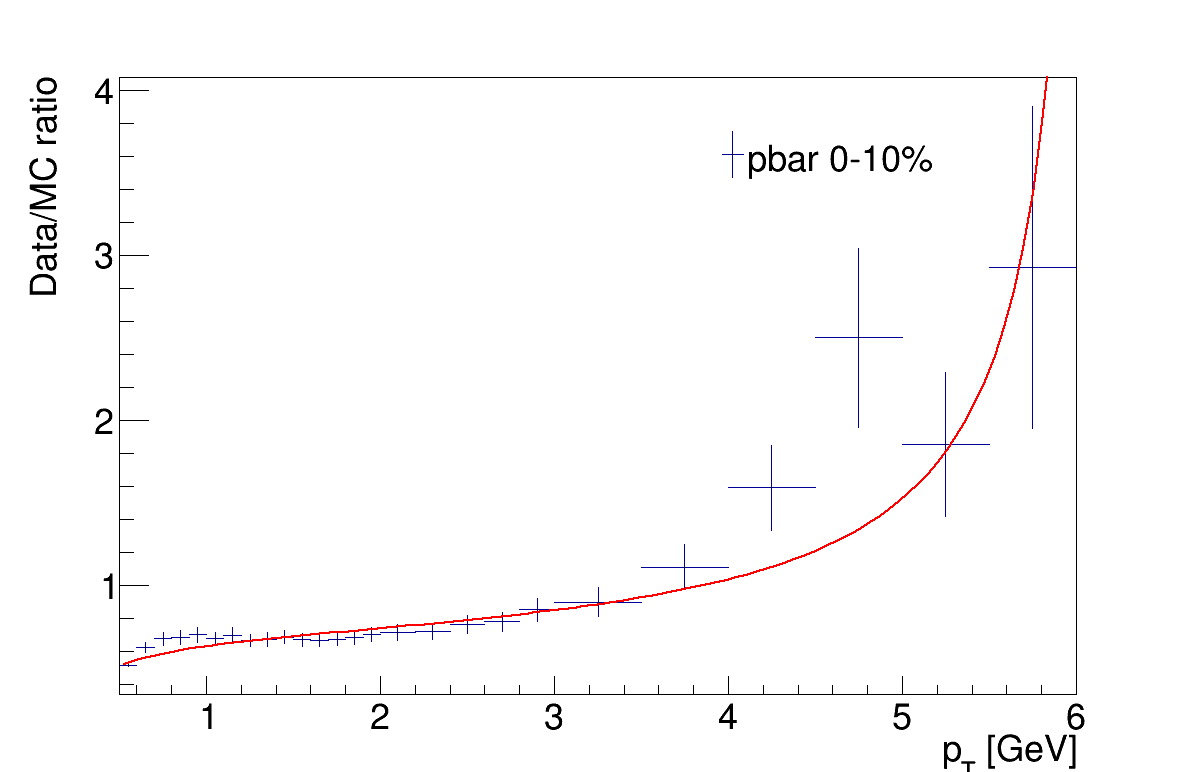
\includegraphics[width=0.24\linewidth]{detdeta/Figures/particle_reweighting_ratios/AMPT_pbar_0.png}
    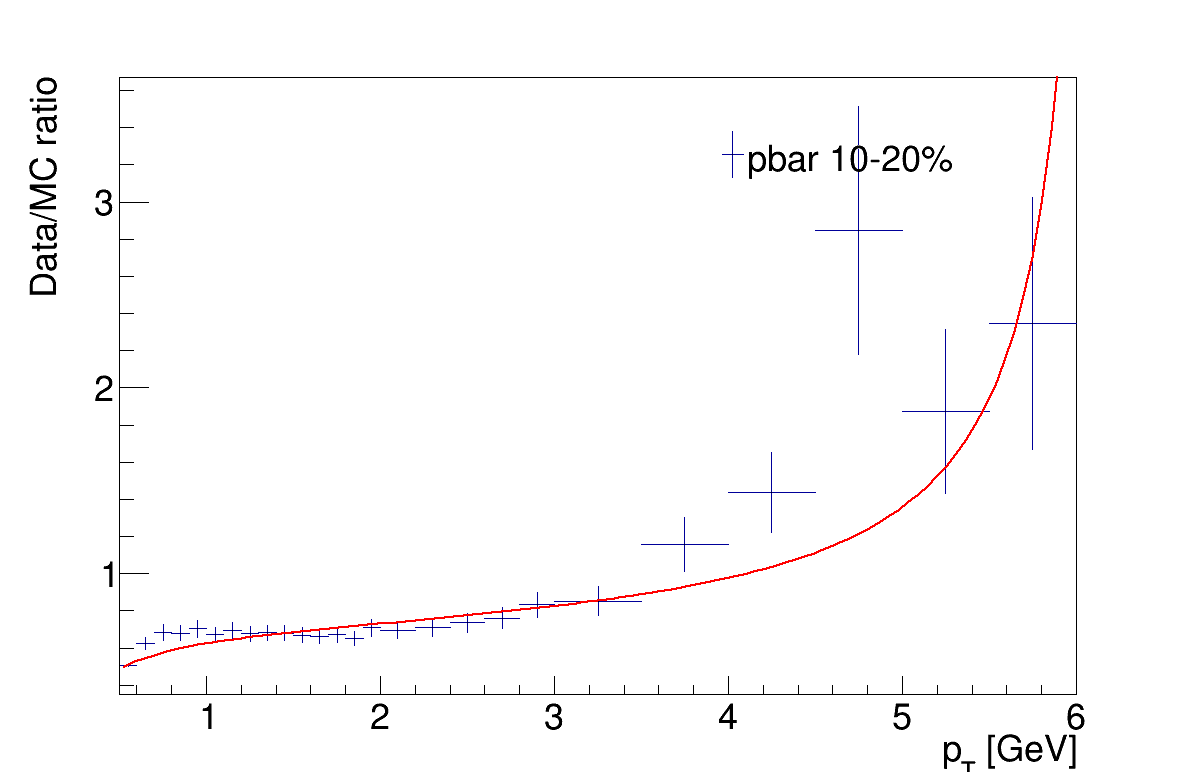
\includegraphics[width=0.24\linewidth]{detdeta/Figures/particle_reweighting_ratios/AMPT_pbar_1.png}
    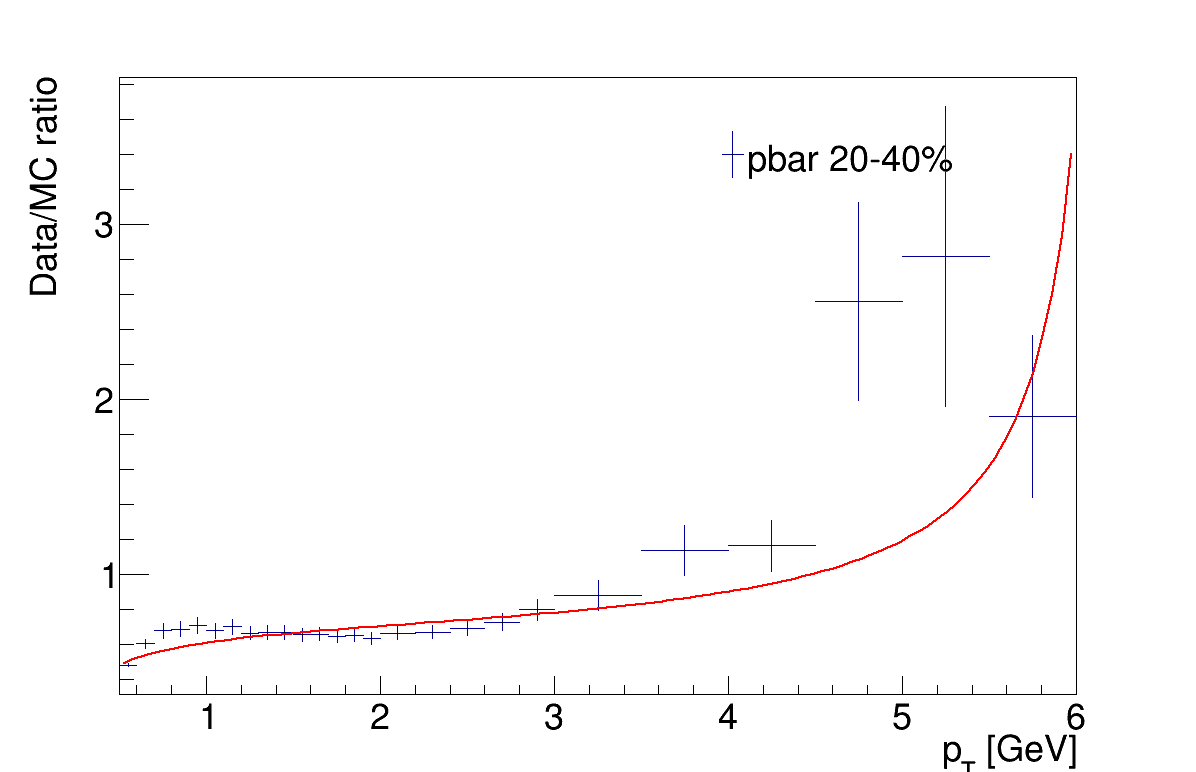
\includegraphics[width=0.24\linewidth]{detdeta/Figures/particle_reweighting_ratios/AMPT_pbar_2.png}
    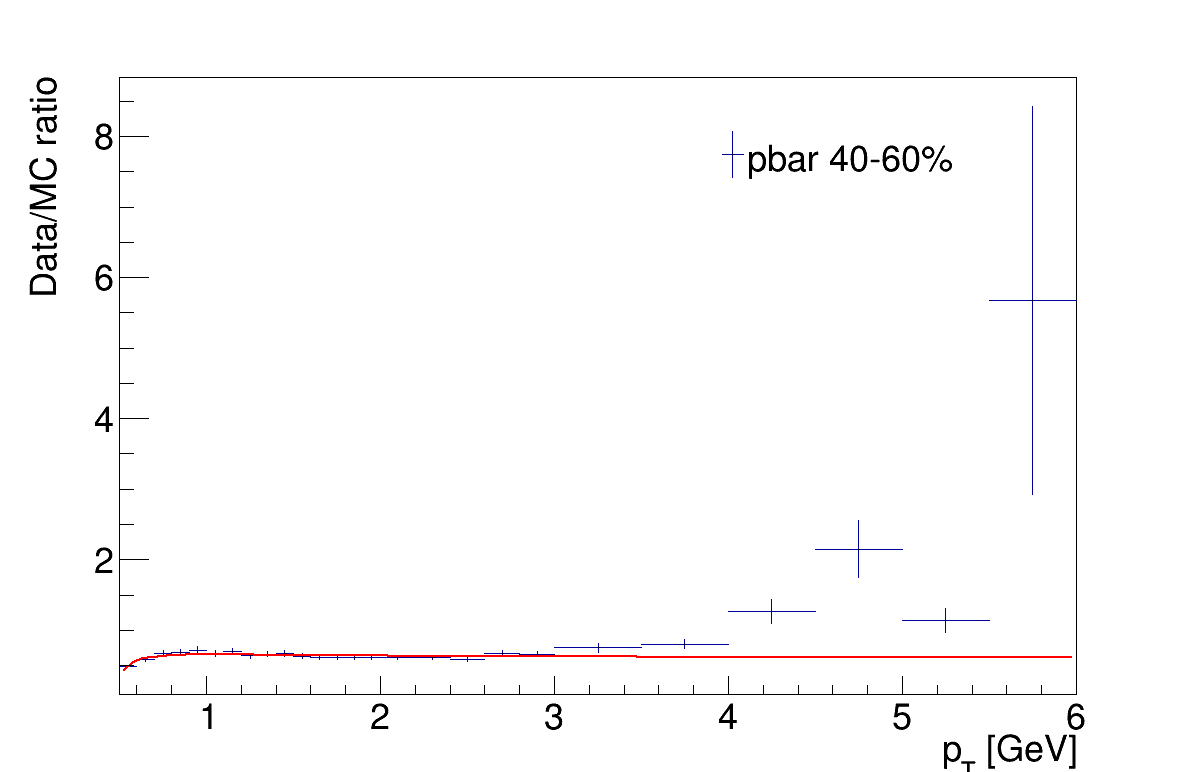
\includegraphics[width=0.24\linewidth]{detdeta/Figures/particle_reweighting_ratios/AMPT_pbar_3.png}
    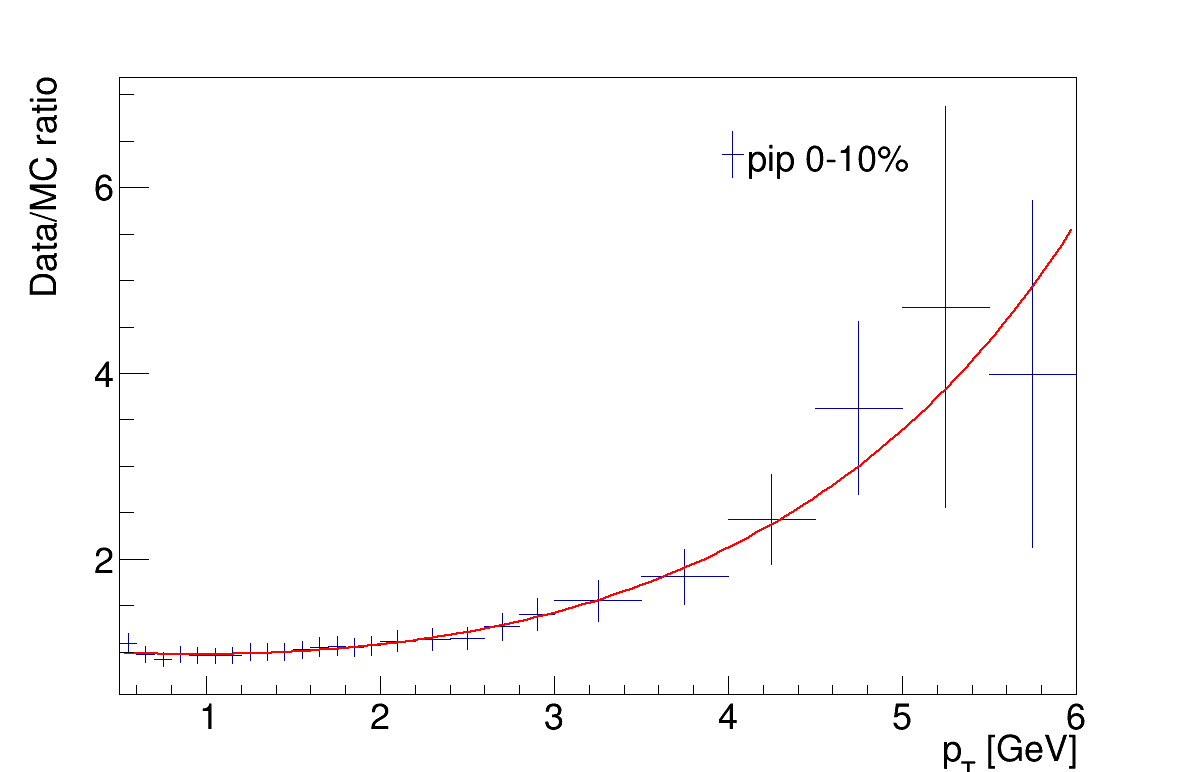
\includegraphics[width=0.24\linewidth]{detdeta/Figures/particle_reweighting_ratios/AMPT_pip_0.png}
    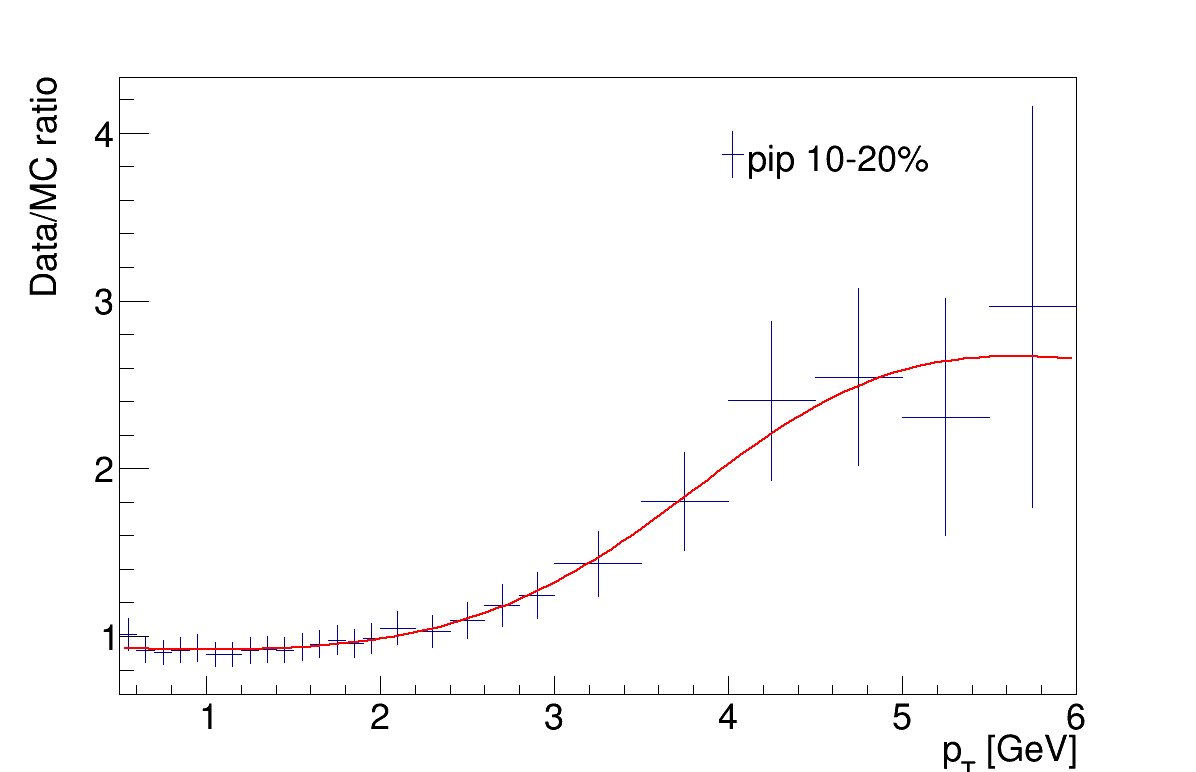
\includegraphics[width=0.24\linewidth]{detdeta/Figures/particle_reweighting_ratios/AMPT_pip_1.png}
    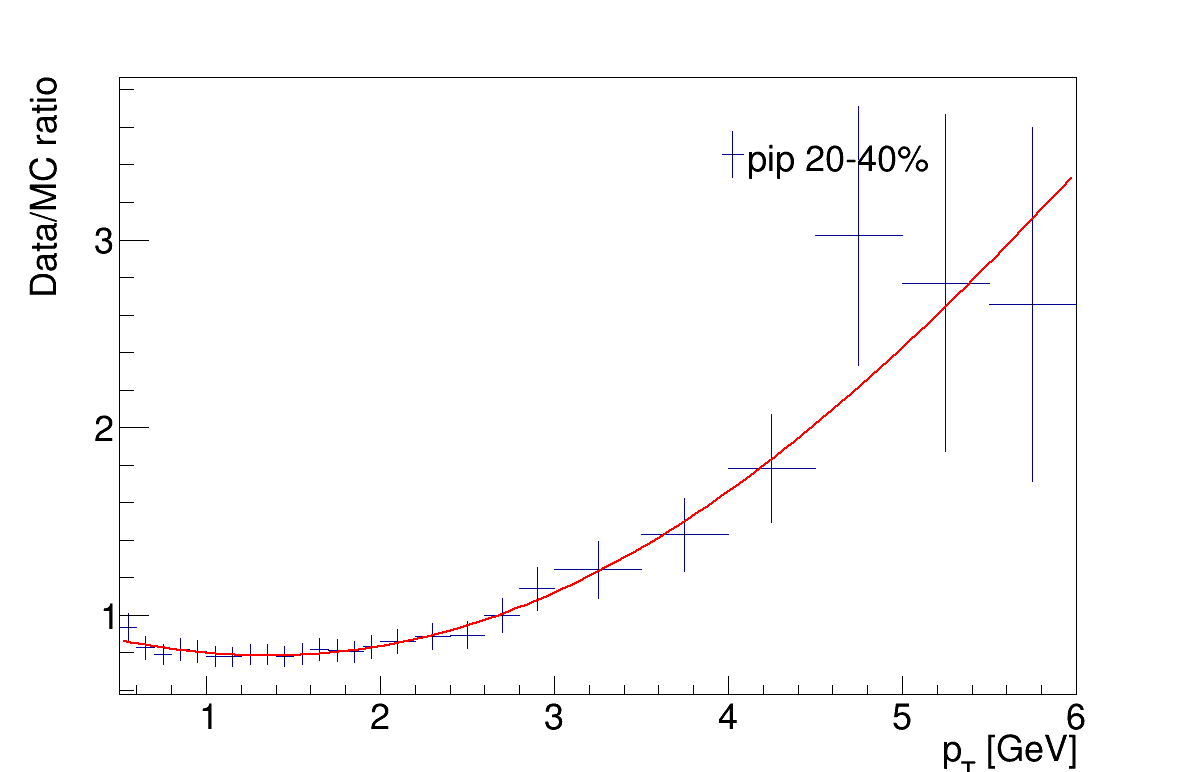
\includegraphics[width=0.24\linewidth]{detdeta/Figures/particle_reweighting_ratios/AMPT_pip_2.png}
    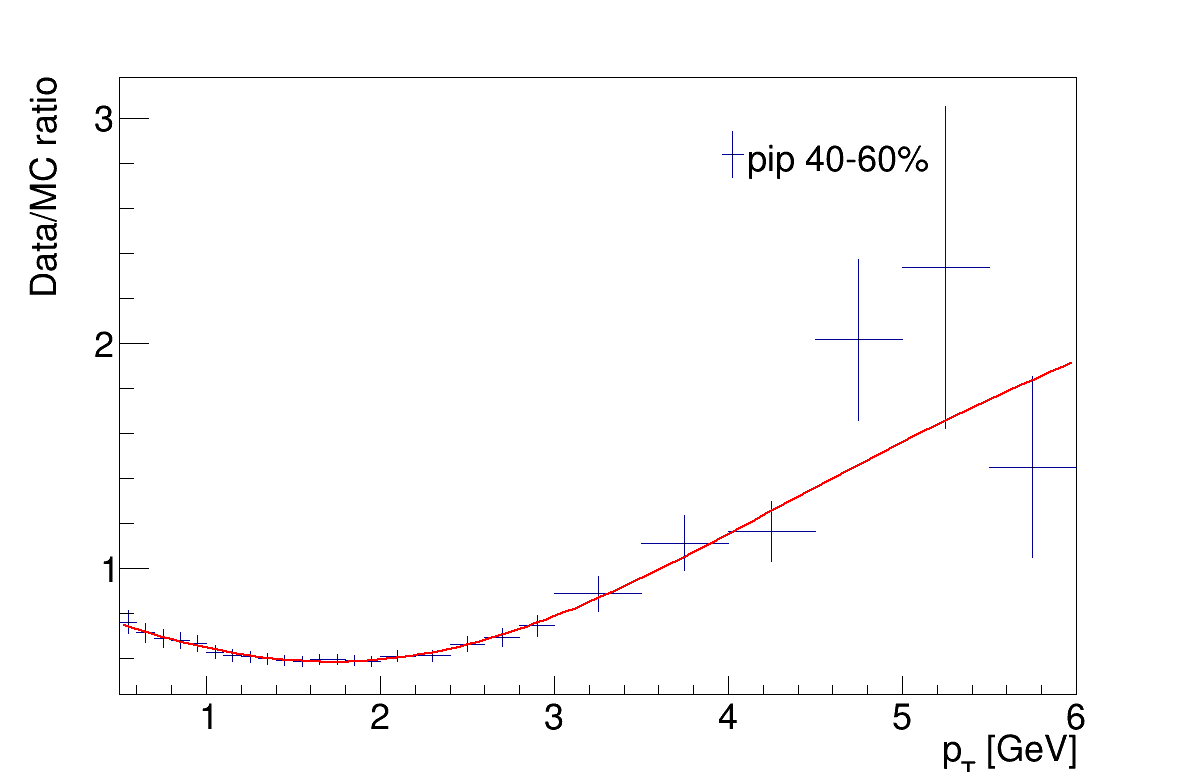
\includegraphics[width=0.24\linewidth]{detdeta/Figures/particle_reweighting_ratios/AMPT_pip_3.png}
    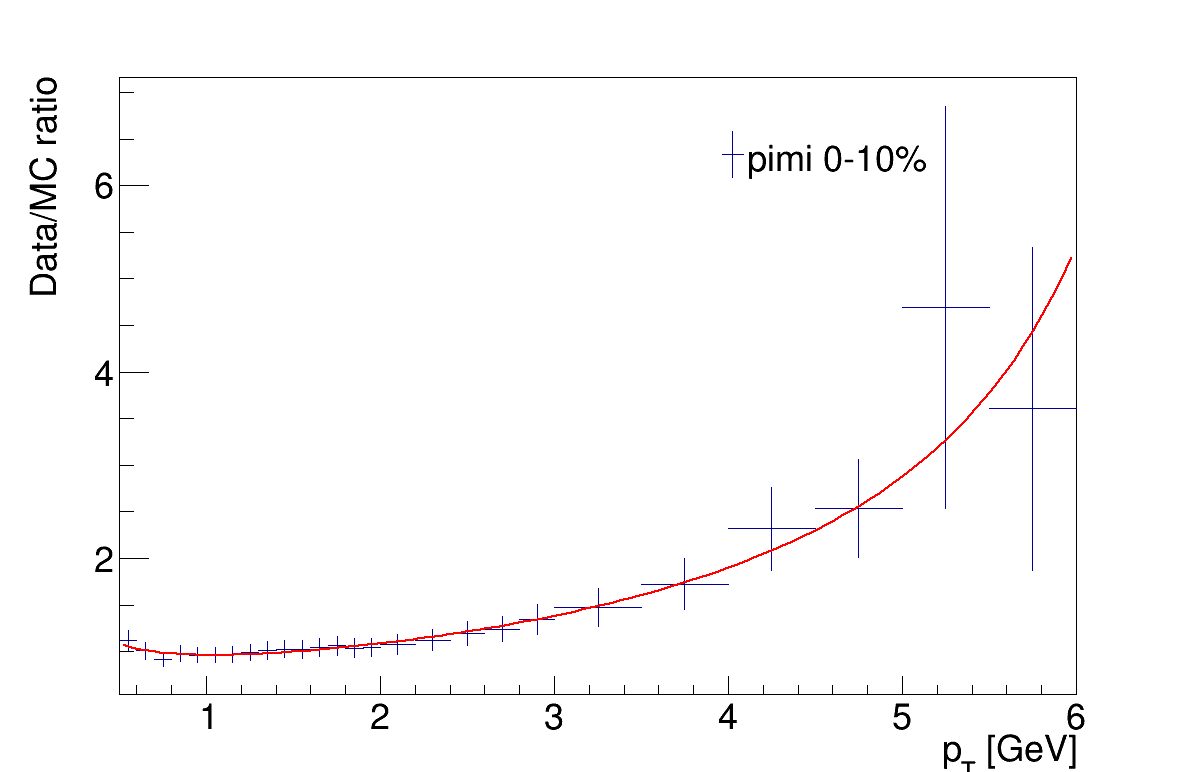
\includegraphics[width=0.24\linewidth]{detdeta/Figures/particle_reweighting_ratios/AMPT_pimi_0.png}
    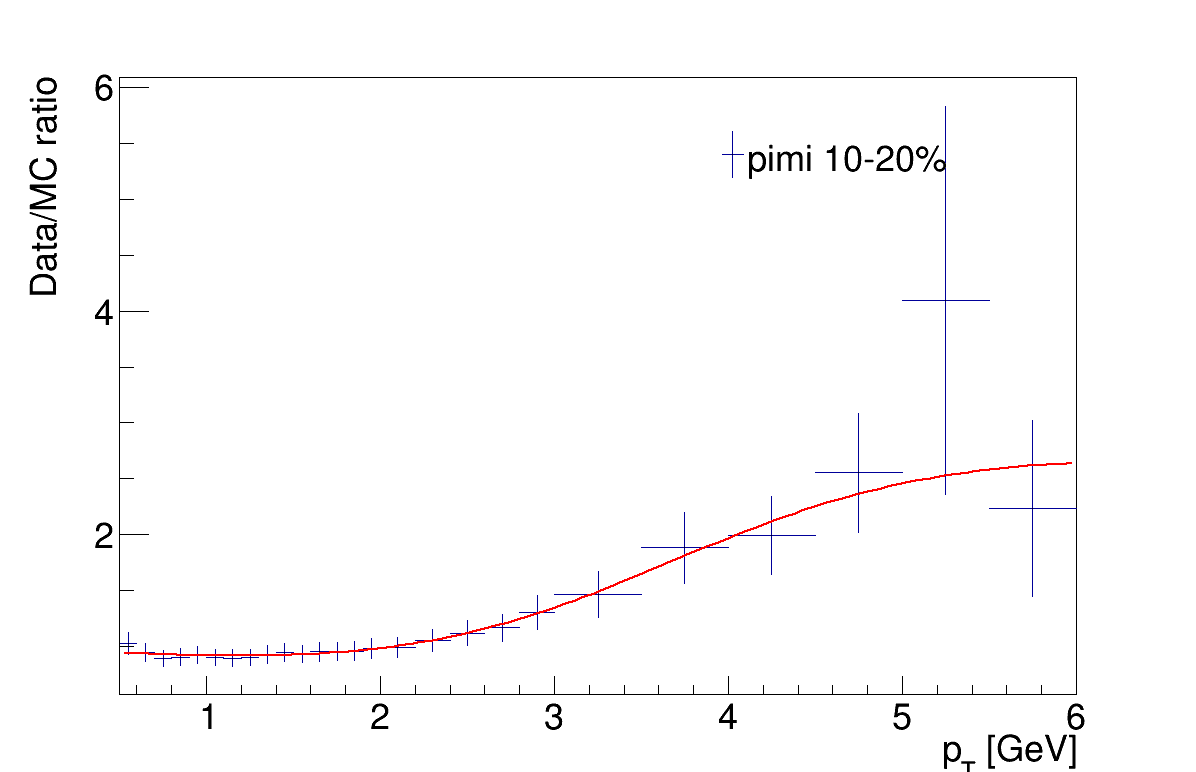
\includegraphics[width=0.24\linewidth]{detdeta/Figures/particle_reweighting_ratios/AMPT_pimi_1.png}
    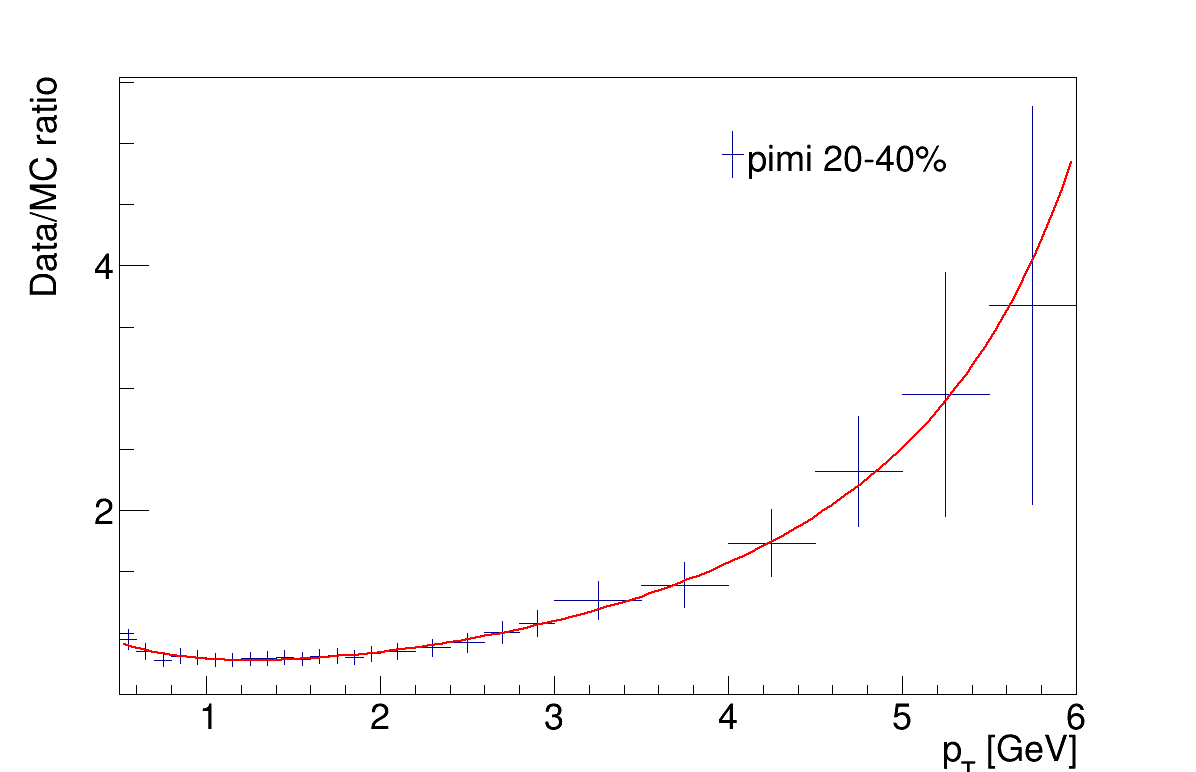
\includegraphics[width=0.24\linewidth]{detdeta/Figures/particle_reweighting_ratios/AMPT_pimi_2.png}
    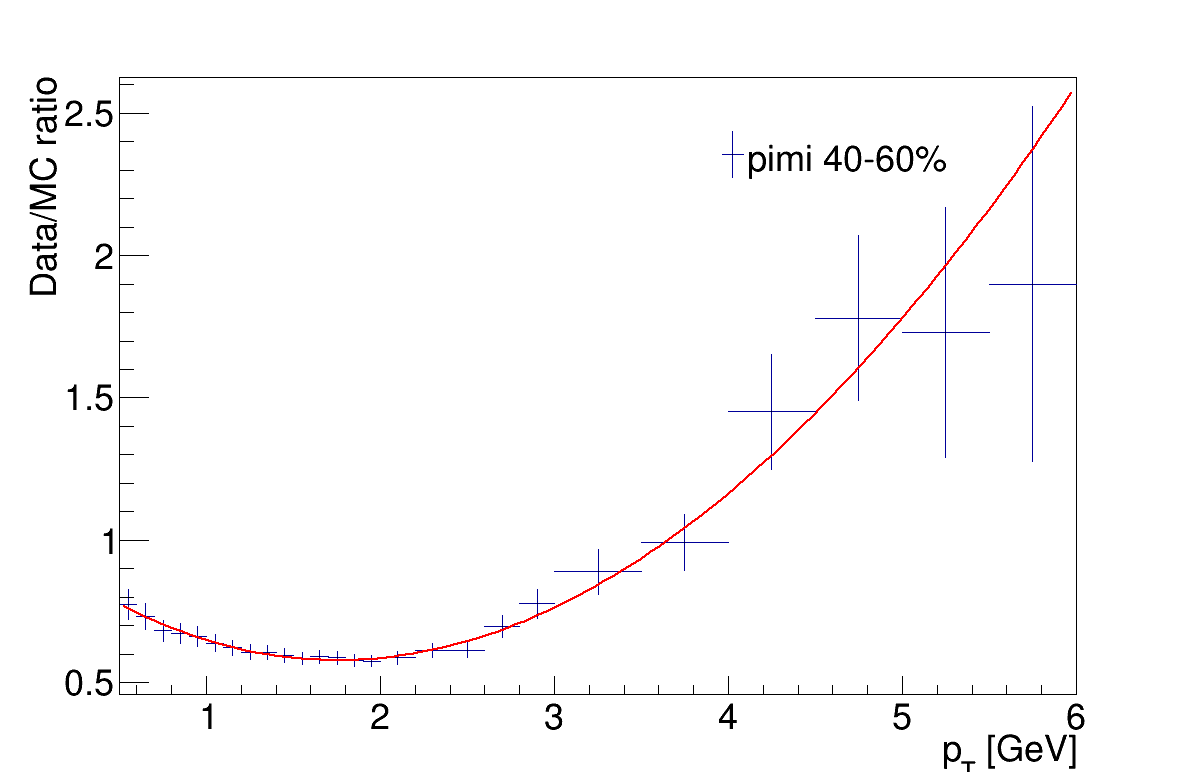
\includegraphics[width=0.24\linewidth]{detdeta/Figures/particle_reweighting_ratios/AMPT_pimi_3.png}
    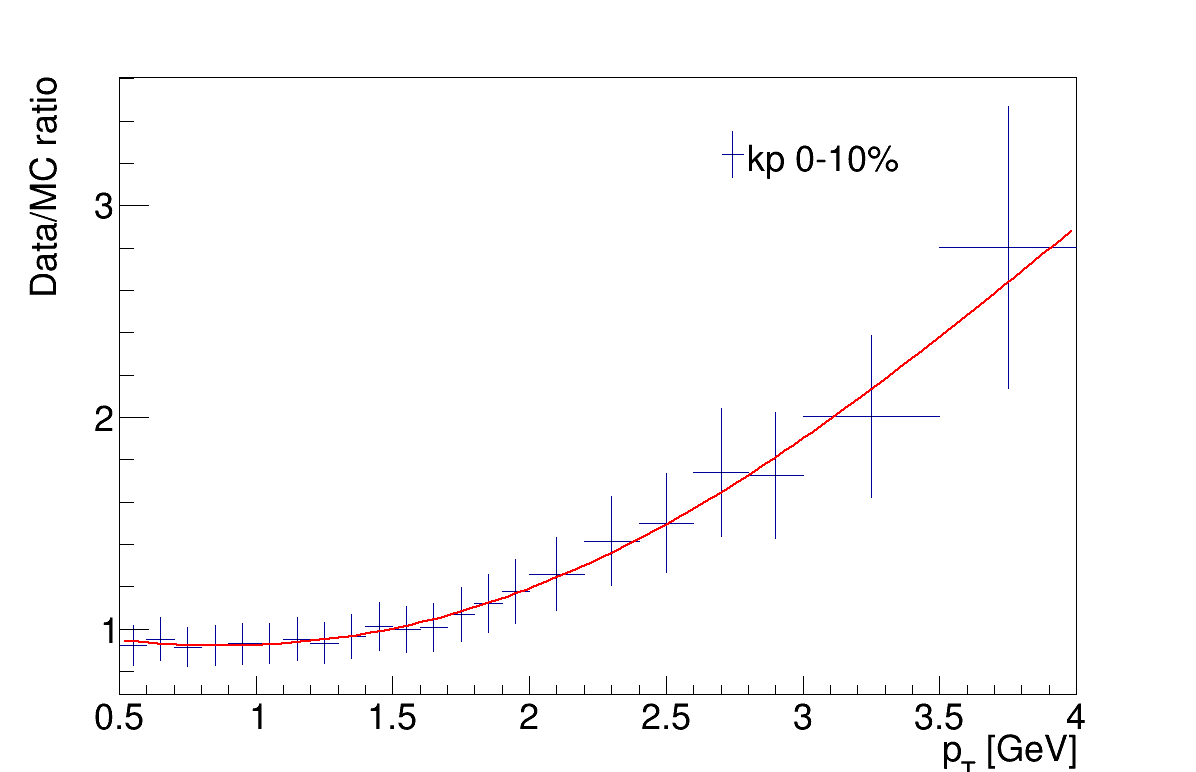
\includegraphics[width=0.24\linewidth]{detdeta/Figures/particle_reweighting_ratios/AMPT_kp_0.png}
    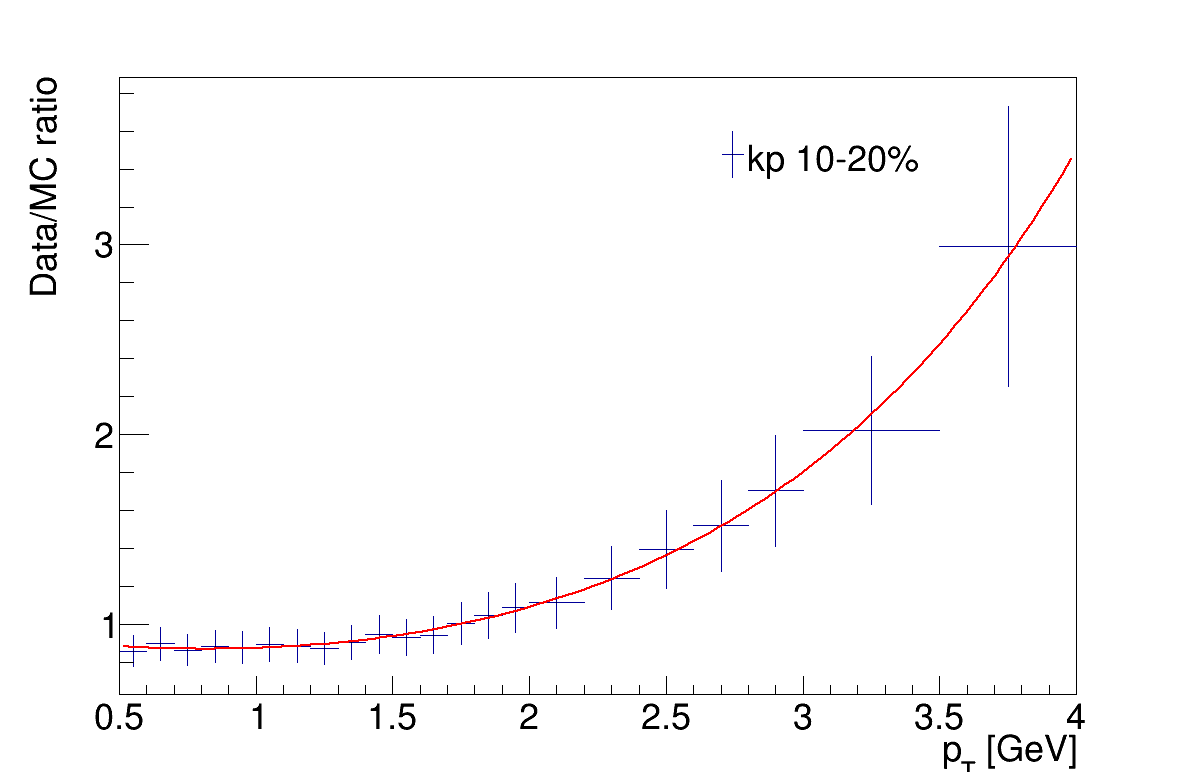
\includegraphics[width=0.24\linewidth]{detdeta/Figures/particle_reweighting_ratios/AMPT_kp_1.png}
    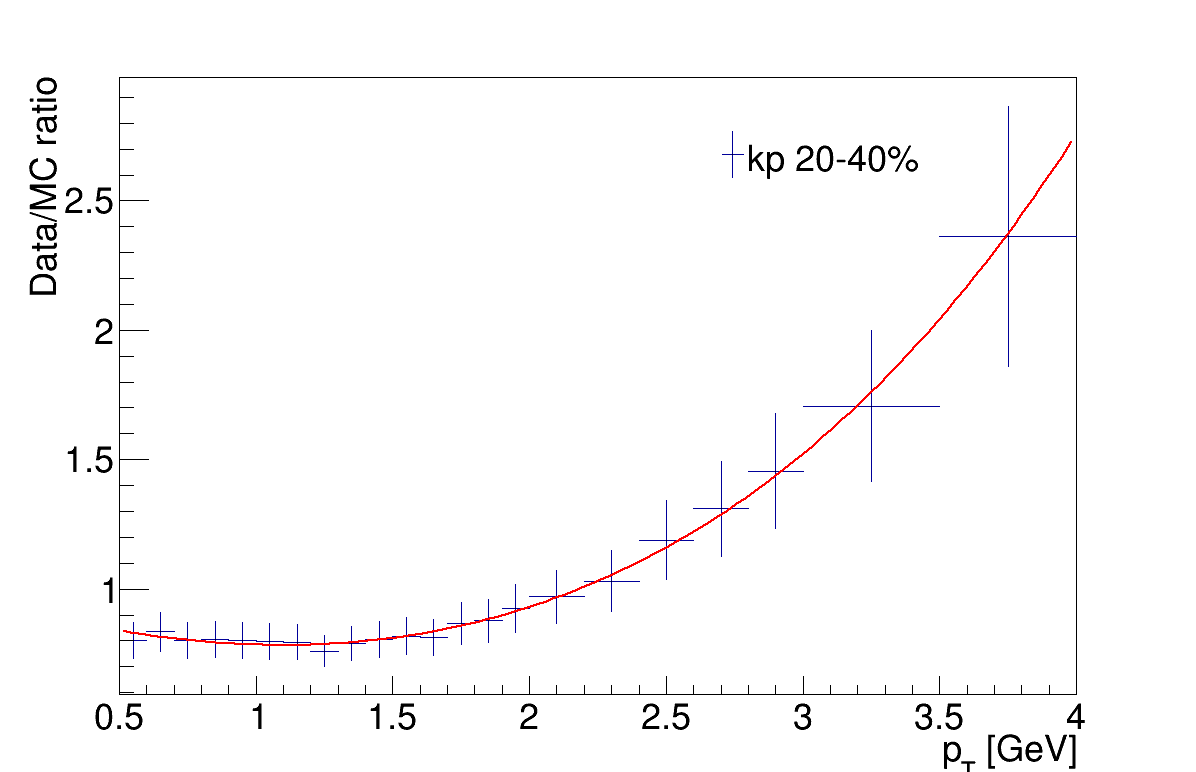
\includegraphics[width=0.24\linewidth]{detdeta/Figures/particle_reweighting_ratios/AMPT_kp_2.png}
    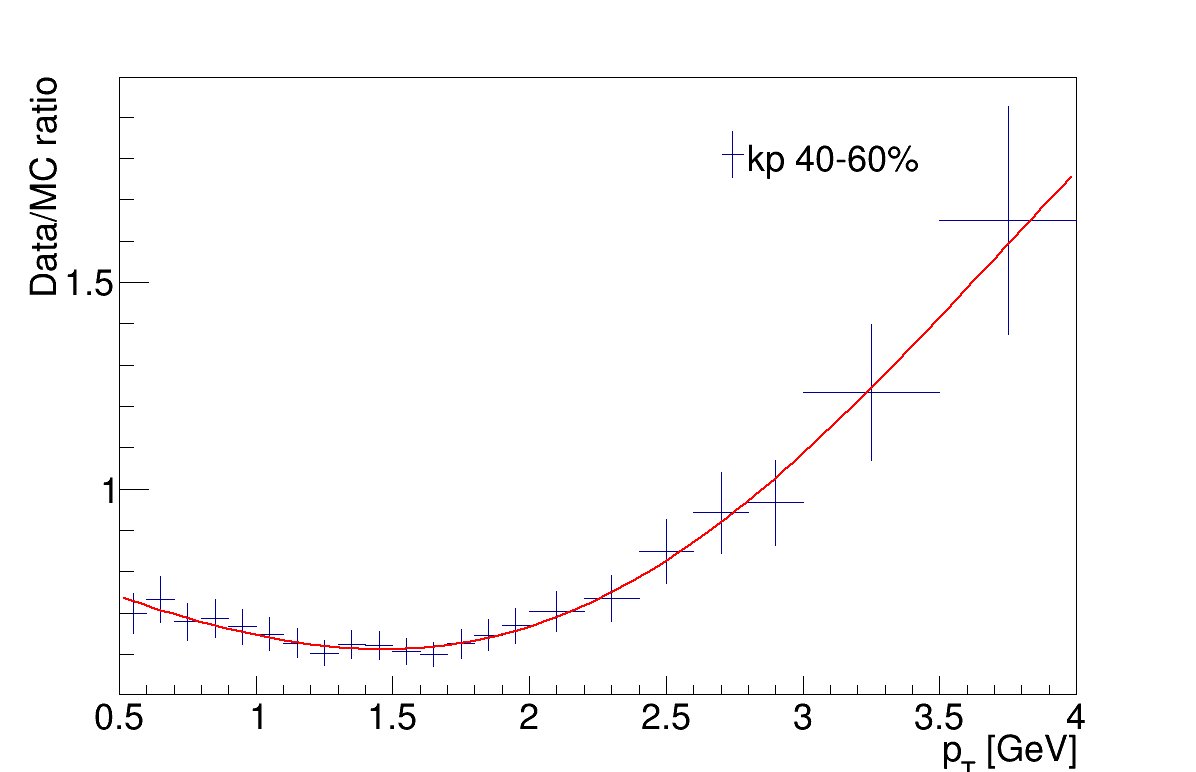
\includegraphics[width=0.24\linewidth]{detdeta/Figures/particle_reweighting_ratios/AMPT_kp_3.png}
    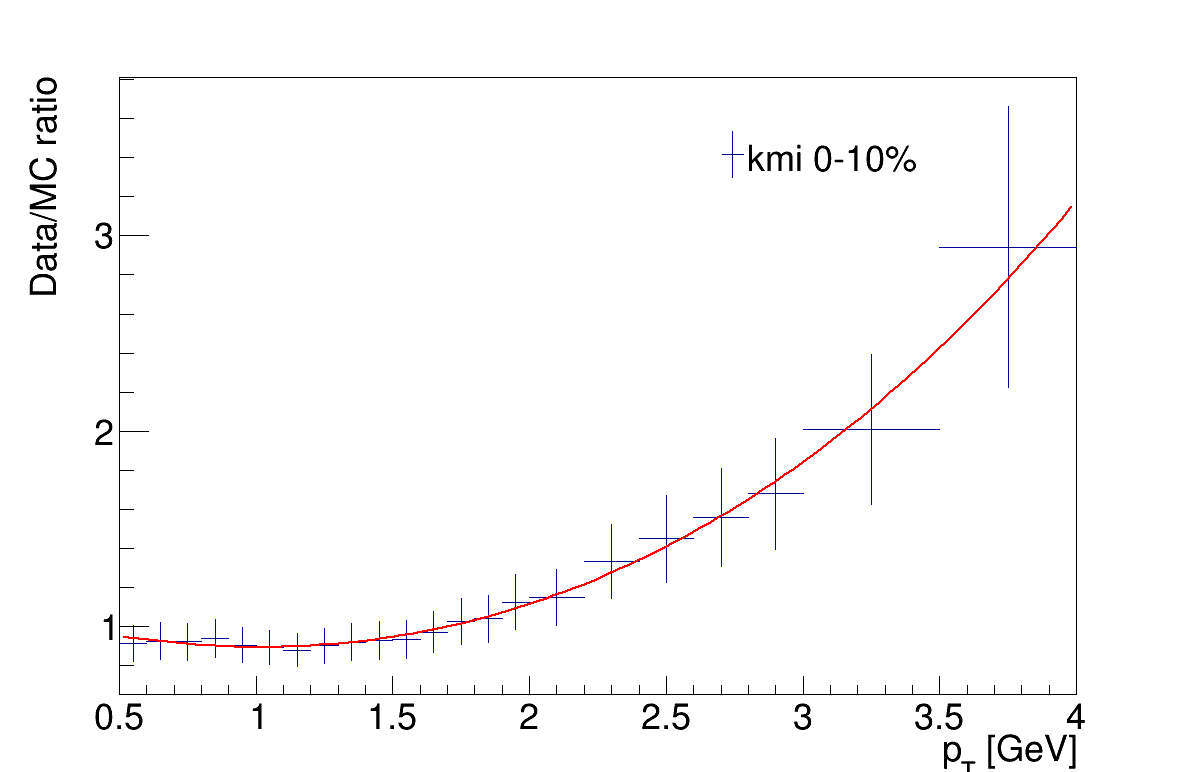
\includegraphics[width=0.24\linewidth]{detdeta/Figures/particle_reweighting_ratios/AMPT_kmi_0.png}
    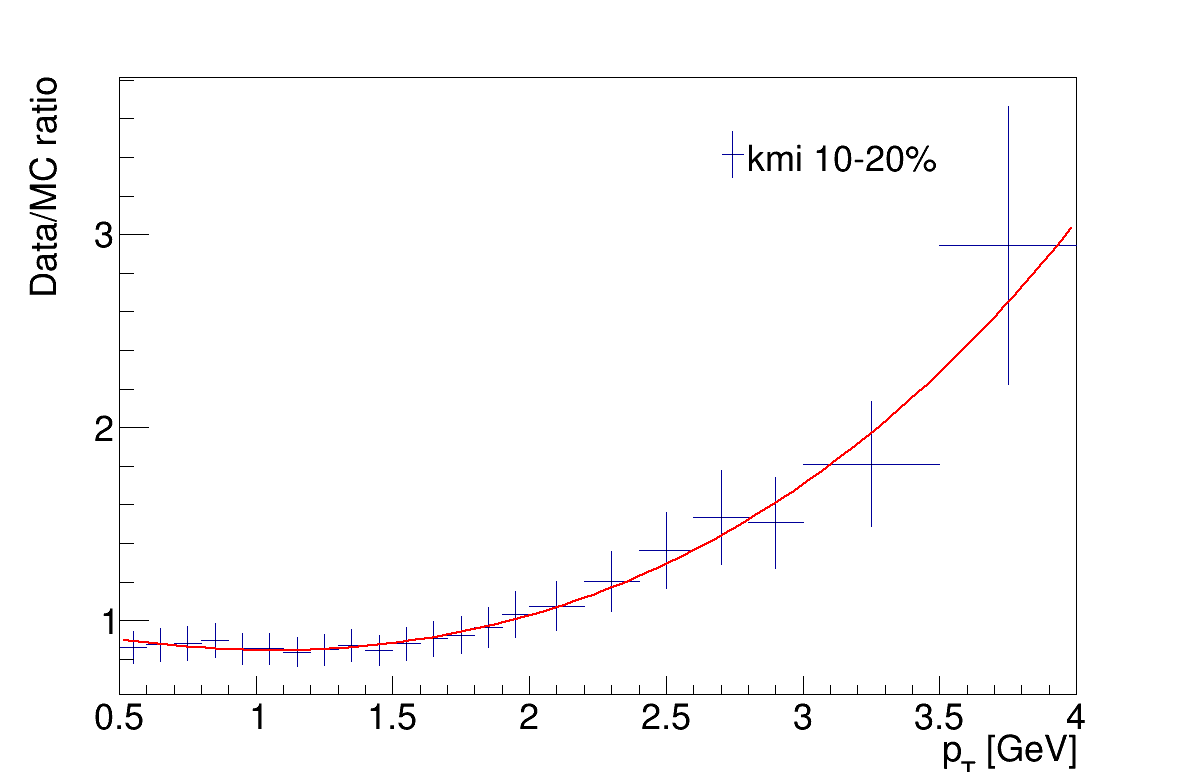
\includegraphics[width=0.24\linewidth]{detdeta/Figures/particle_reweighting_ratios/AMPT_kmi_1.png}
    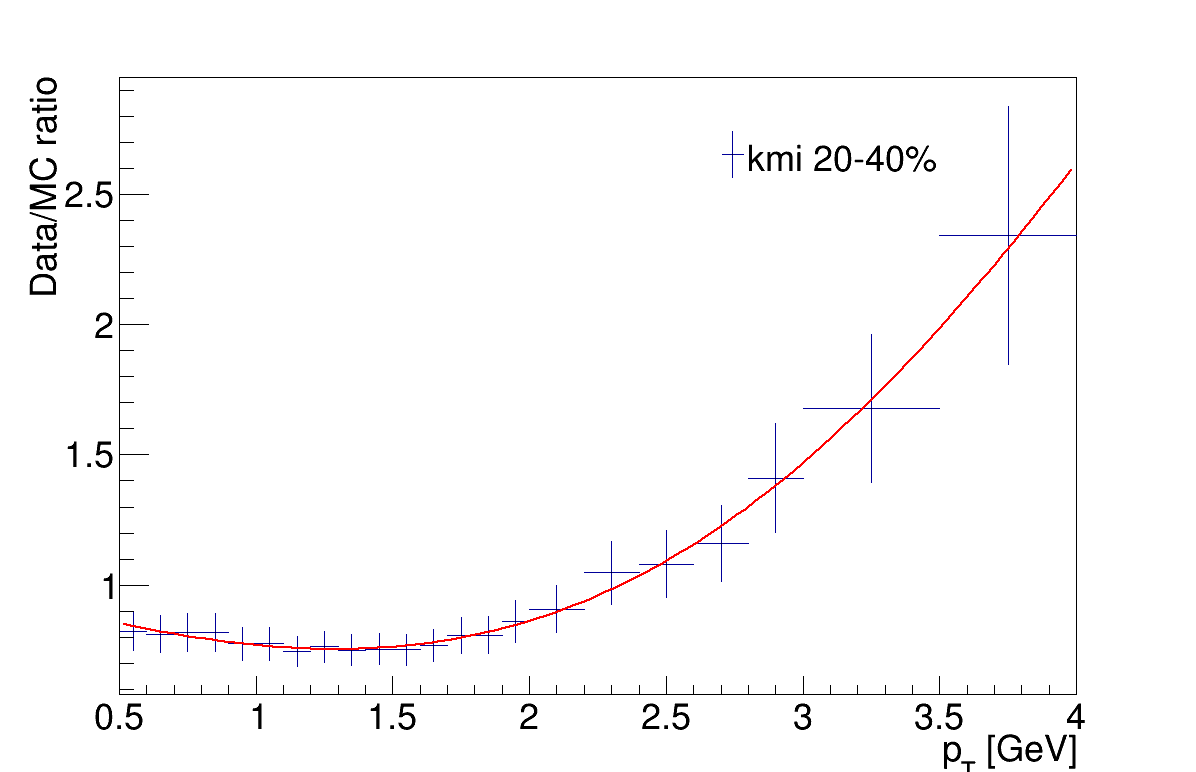
\includegraphics[width=0.24\linewidth]{detdeta/Figures/particle_reweighting_ratios/AMPT_kmi_2.png}
    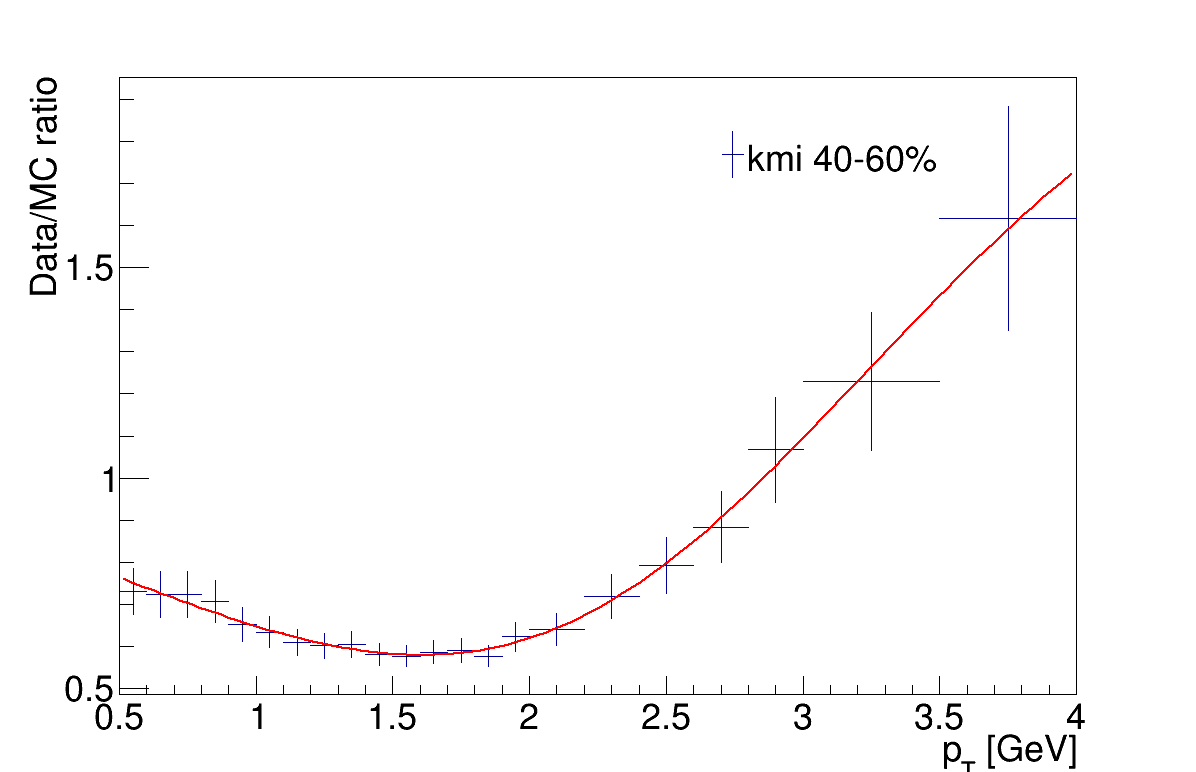
\includegraphics[width=0.24\linewidth]{detdeta/Figures/particle_reweighting_ratios/AMPT_kmi_3.png}
    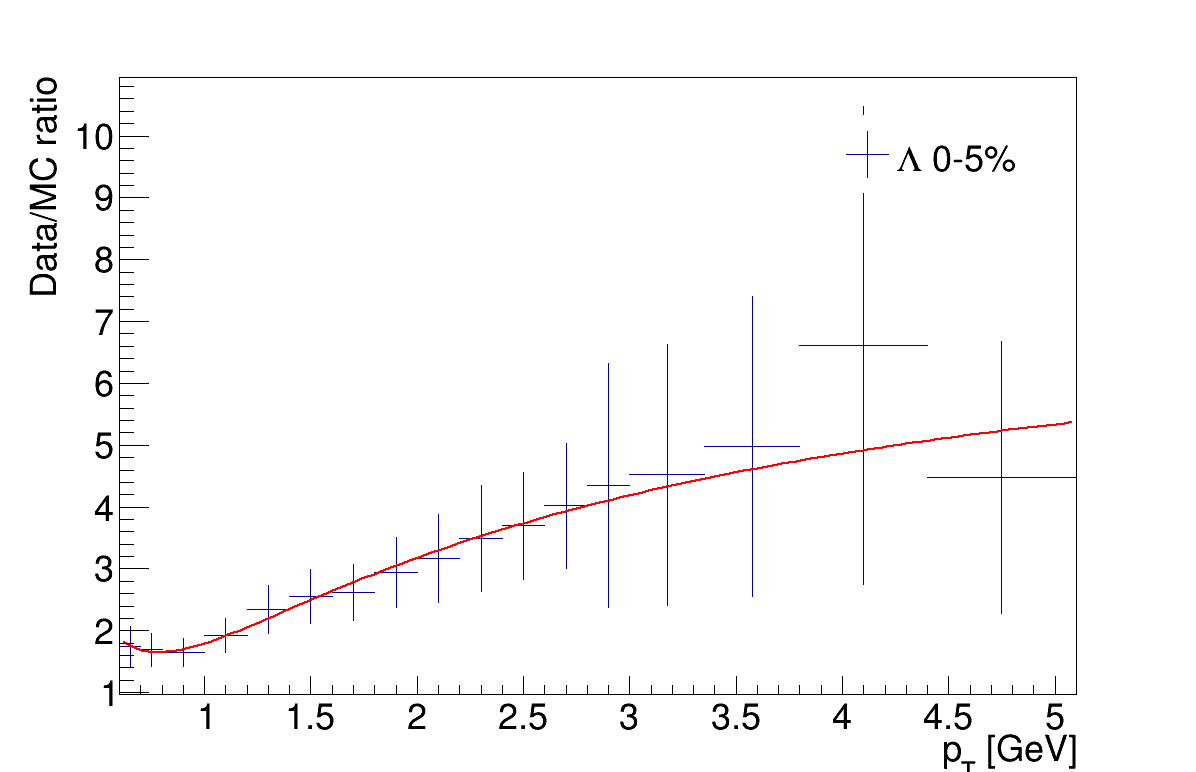
\includegraphics[width=0.24\linewidth]{detdeta/Figures/particle_reweighting_ratios/AMPT_lambda_0.png}
    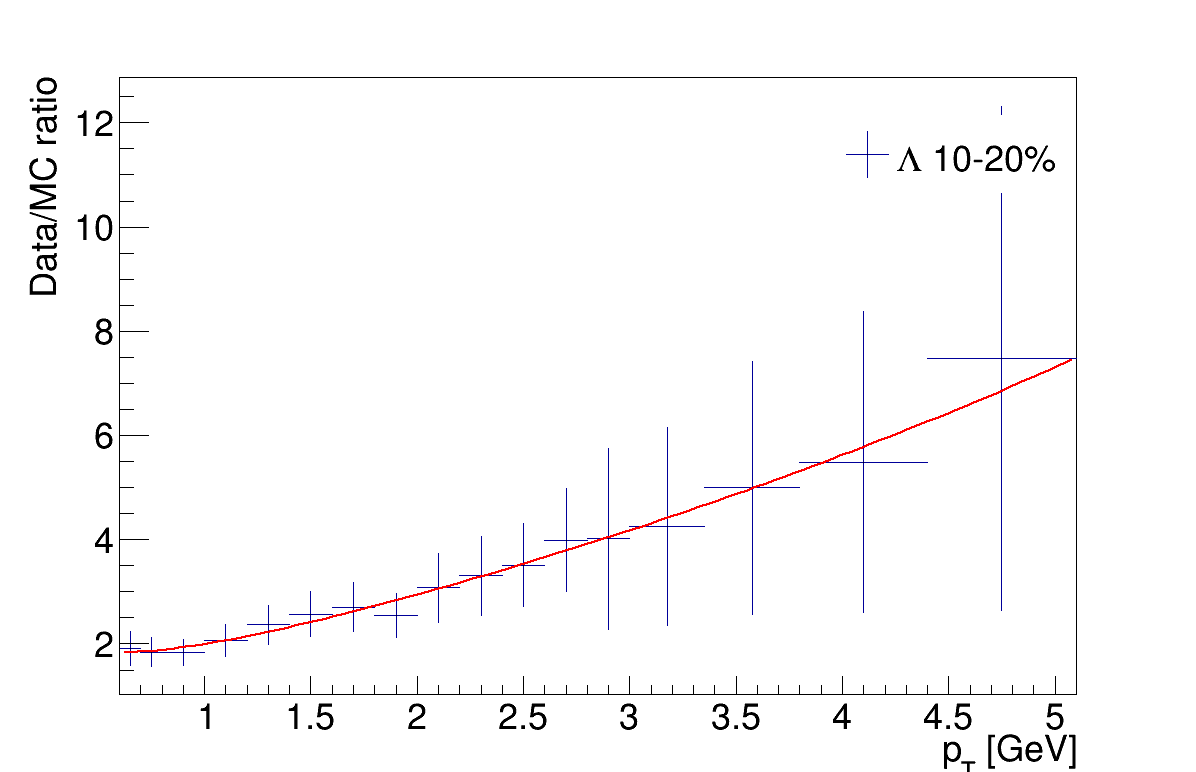
\includegraphics[width=0.24\linewidth]{detdeta/Figures/particle_reweighting_ratios/AMPT_lambda_1.png}
    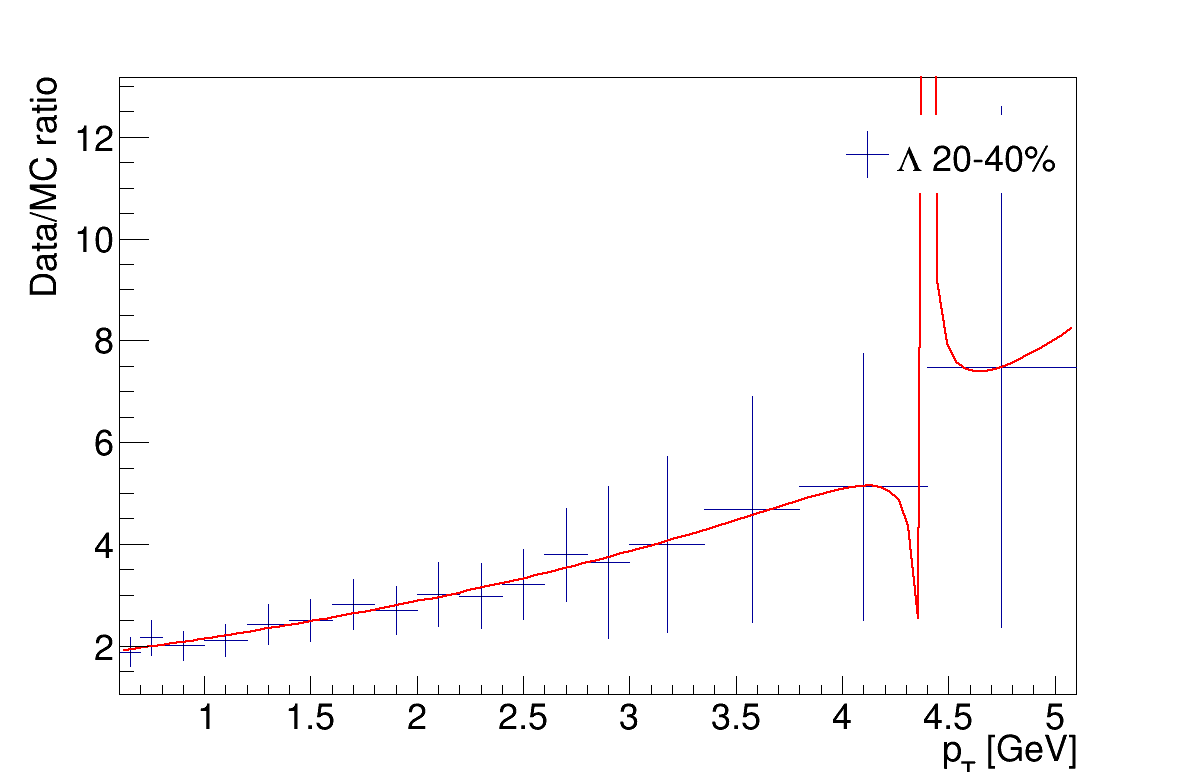
\includegraphics[width=0.24\linewidth]{detdeta/Figures/particle_reweighting_ratios/AMPT_lambda_2.png}
    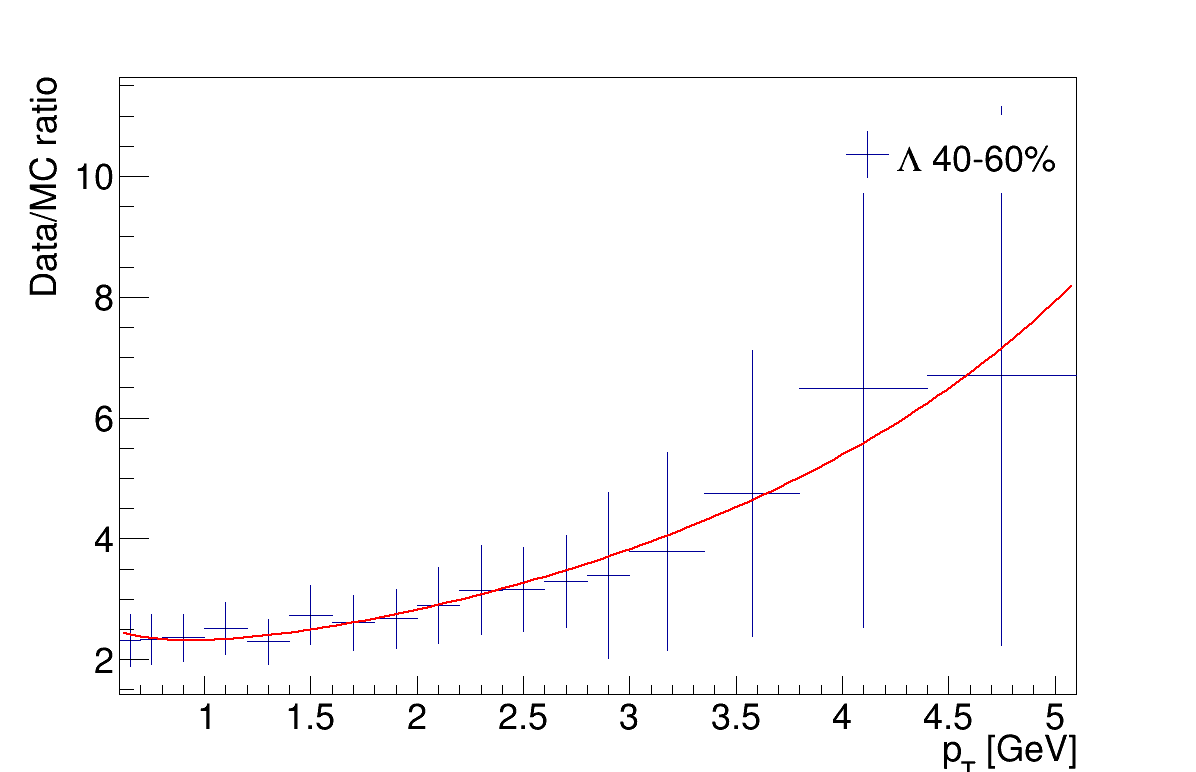
\includegraphics[width=0.24\linewidth]{detdeta/Figures/particle_reweighting_ratios/AMPT_lambda_3.png}
    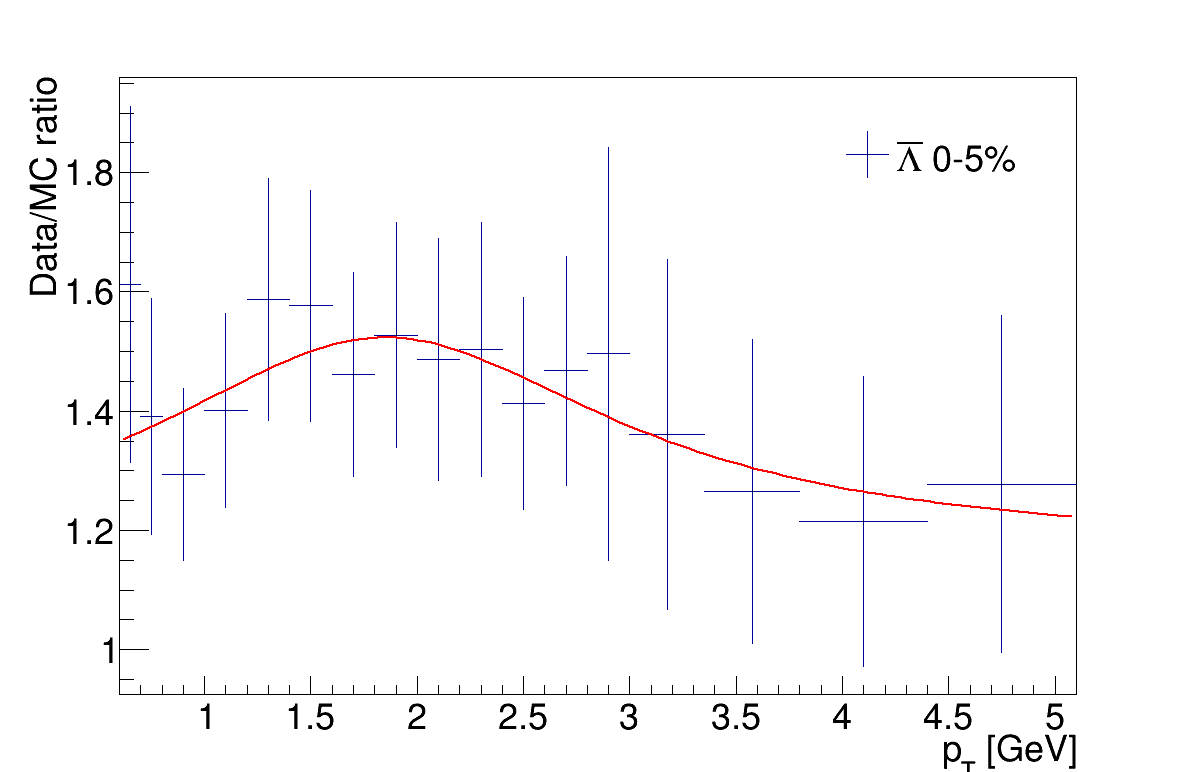
\includegraphics[width=0.24\linewidth]{detdeta/Figures/particle_reweighting_ratios/AMPT_lambda_bar_0.png}
    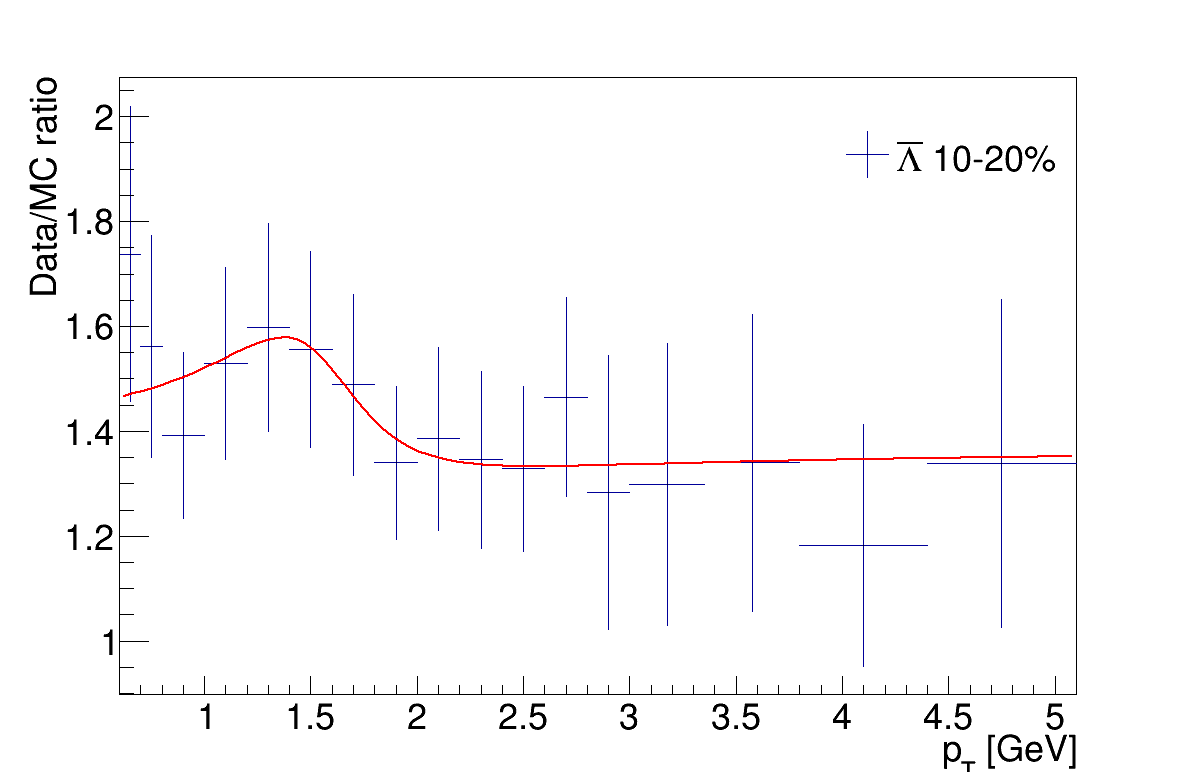
\includegraphics[width=0.24\linewidth]{detdeta/Figures/particle_reweighting_ratios/AMPT_lambda_bar_1.png}
    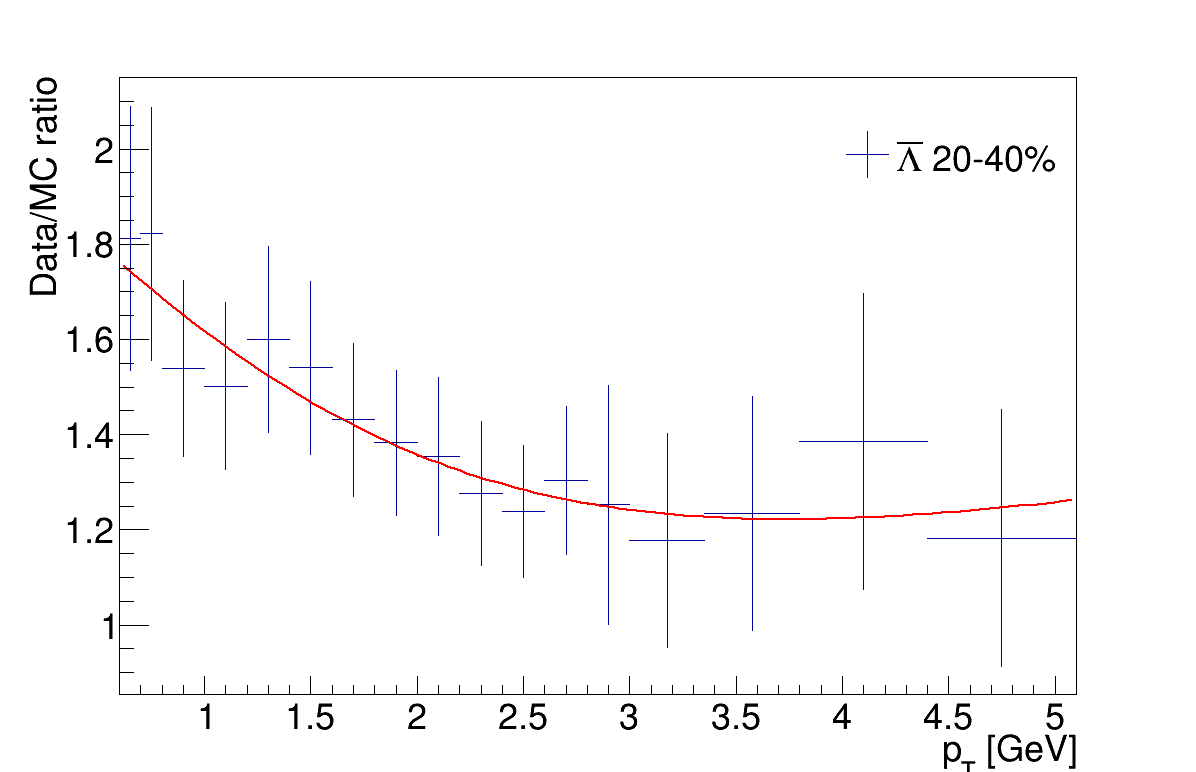
\includegraphics[width=0.24\linewidth]{detdeta/Figures/particle_reweighting_ratios/AMPT_lambda_bar_2.png}
    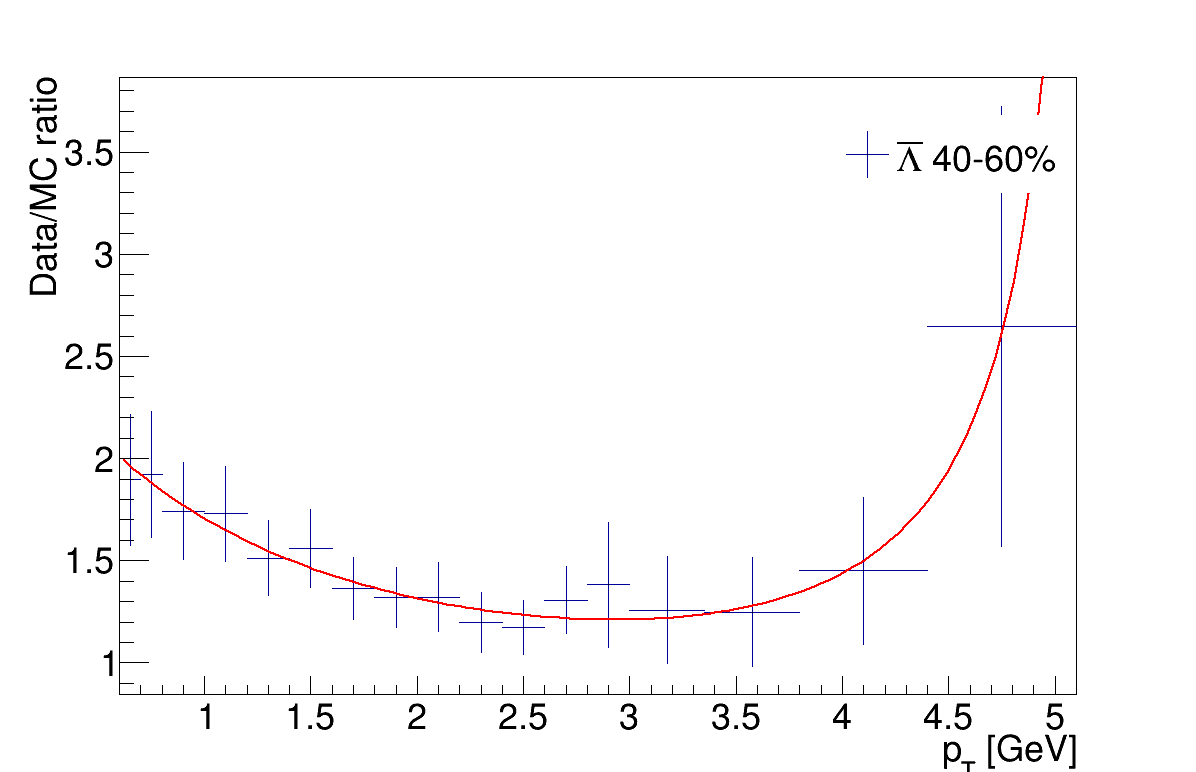
\includegraphics[width=0.24\linewidth]{detdeta/Figures/particle_reweighting_ratios/AMPT_lambda_bar_3.png}
    \caption{All data to MC ratios used in nominal AMPT reweighting method for protons, anti-protons, kaons, pions and lambda particles.}
    \label{fig:ampt_data_mc_particle_ratios}
\end{figure}

The effect of this particle reweighting methodology on the correction factors used to correct the detector-level \detdeta to truth-level \detdeta is shown in Fig.~\ref{fig:reweighted_corr_factors} for the EMCal, HCal and full calorimeter measurements. 
Fig.~\ref{fig:reweighted_corr_ratio} gives the ratio of the unweighted and reweighted correction factors.
\begin{figure}
    \centering
    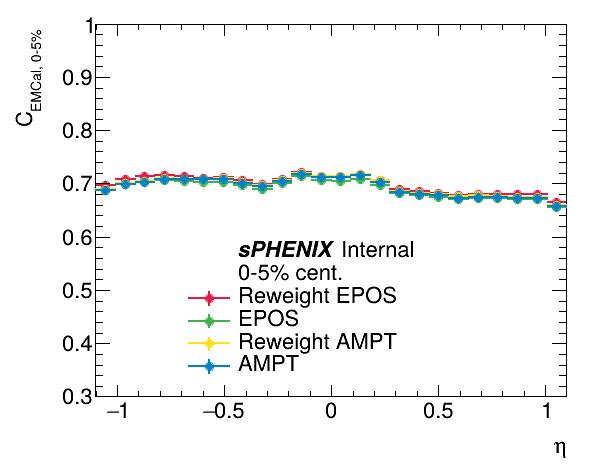
\includegraphics[width=0.24\linewidth]{detdeta/Figures/particle_reweighting_ratios/emcal_corr_0-5.png}
    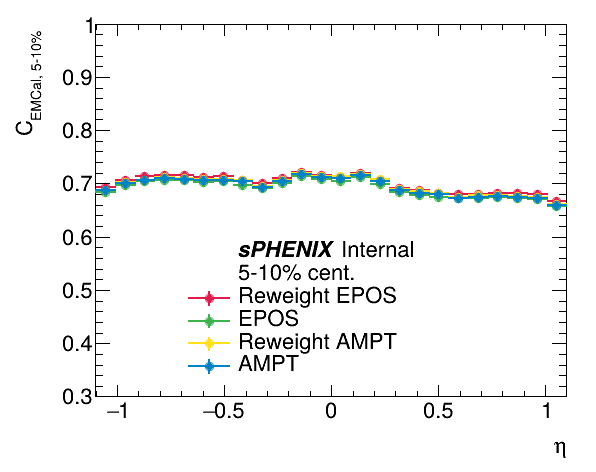
\includegraphics[width=0.24\linewidth]{detdeta/Figures/particle_reweighting_ratios/emcal_corr_5-10.png}
    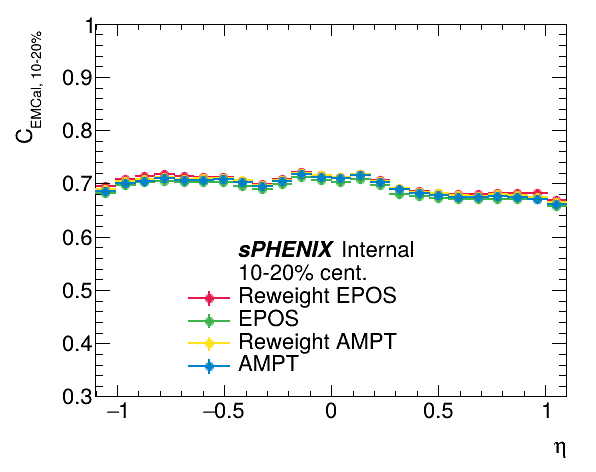
\includegraphics[width=0.24\linewidth]{detdeta/Figures/particle_reweighting_ratios/emcal_corr_10-20.png}
    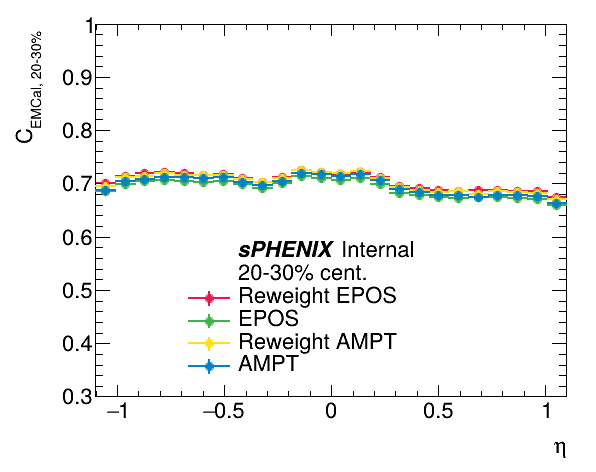
\includegraphics[width=0.24\linewidth]{detdeta/Figures/particle_reweighting_ratios/emcal_corr_20-30.png}
    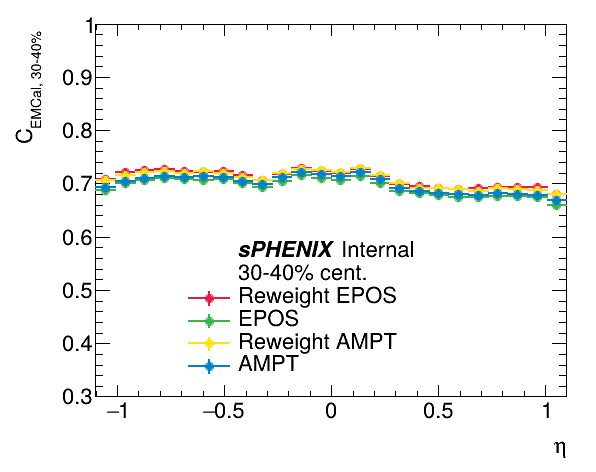
\includegraphics[width=0.24\linewidth]{detdeta/Figures/particle_reweighting_ratios/emcal_corr_30-40.png}
    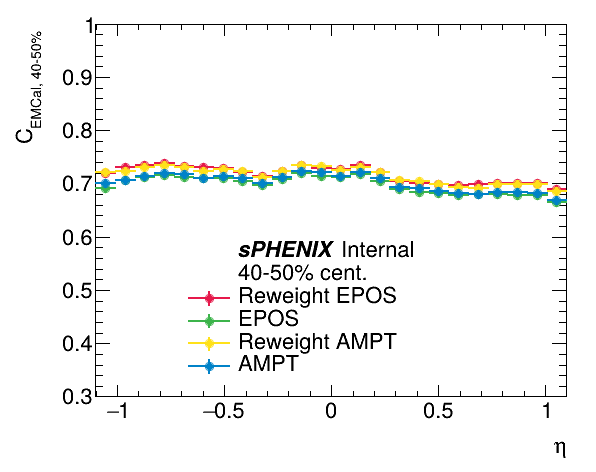
\includegraphics[width=0.24\linewidth]{detdeta/Figures/particle_reweighting_ratios/emcal_corr_40-50.png}
    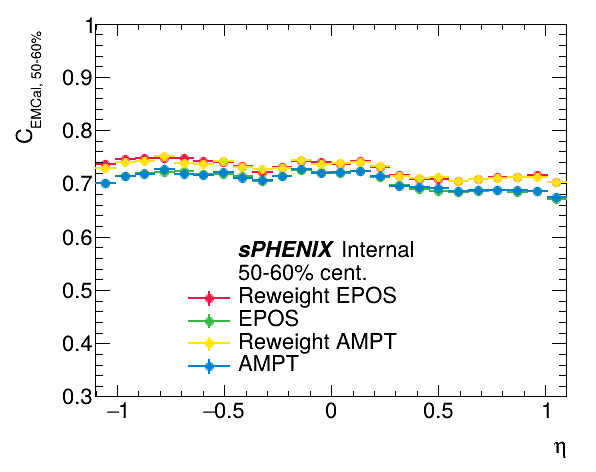
\includegraphics[width=0.24\linewidth]{detdeta/Figures/particle_reweighting_ratios/emcal_corr_50-60.png} \\
    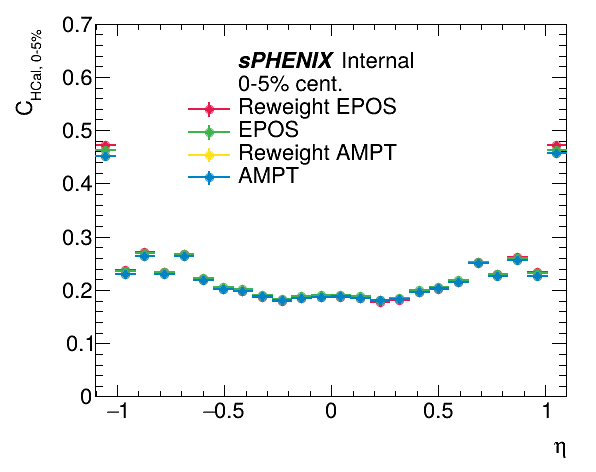
\includegraphics[width=0.24\linewidth]{detdeta/Figures/particle_reweighting_ratios/hcal_corr_0-5.png}
    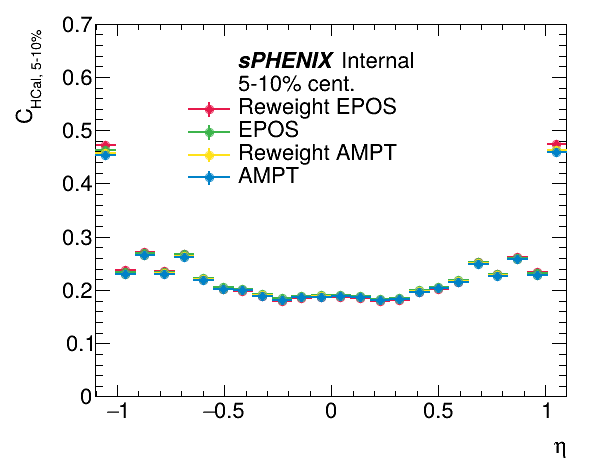
\includegraphics[width=0.24\linewidth]{detdeta/Figures/particle_reweighting_ratios/hcal_corr_5-10.png}
    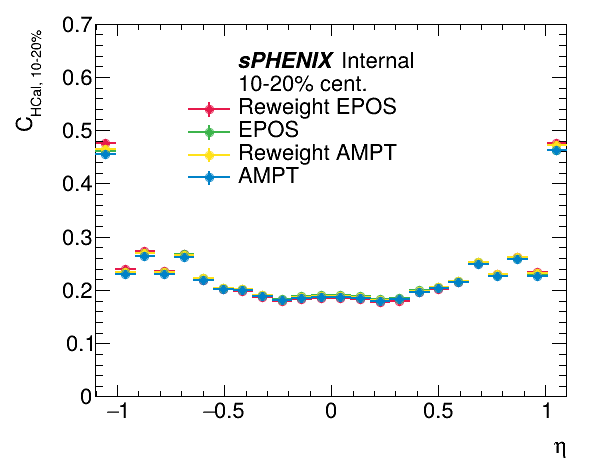
\includegraphics[width=0.24\linewidth]{detdeta/Figures/particle_reweighting_ratios/hcal_corr_10-20.png}
    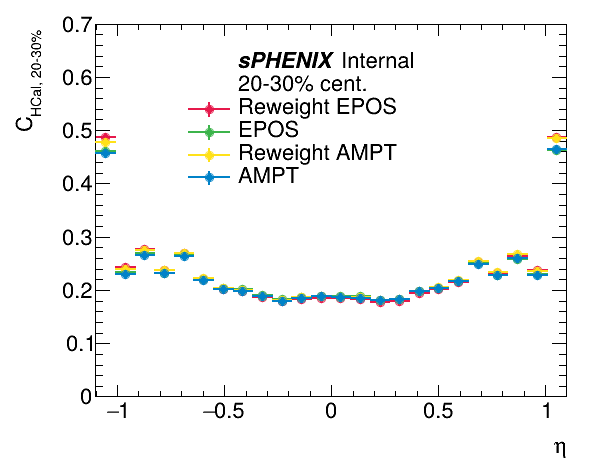
\includegraphics[width=0.24\linewidth]{detdeta/Figures/particle_reweighting_ratios/hcal_corr_20-30.png}
    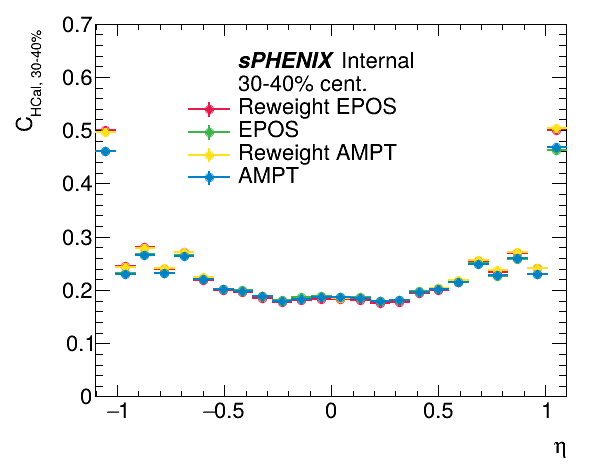
\includegraphics[width=0.24\linewidth]{detdeta/Figures/particle_reweighting_ratios/hcal_corr_30-40.png}
    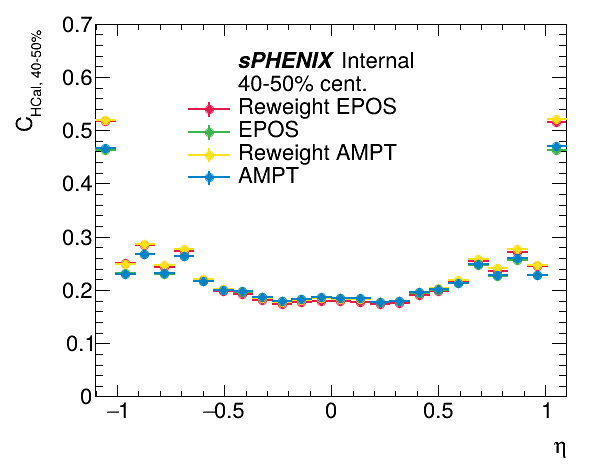
\includegraphics[width=0.24\linewidth]{detdeta/Figures/particle_reweighting_ratios/hcal_corr_40-50.png}
    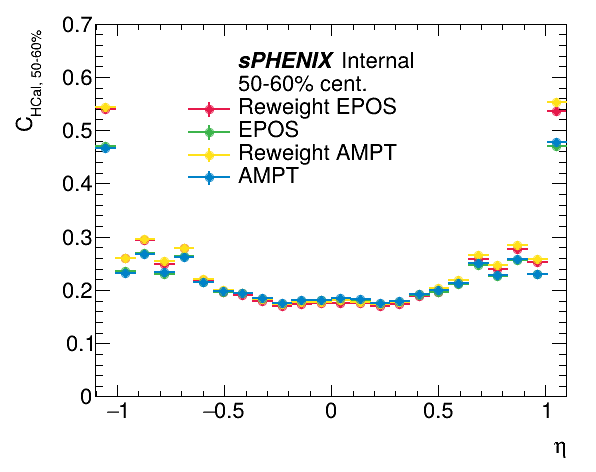
\includegraphics[width=0.24\linewidth]{detdeta/Figures/particle_reweighting_ratios/hcal_corr_50-60.png} \\
    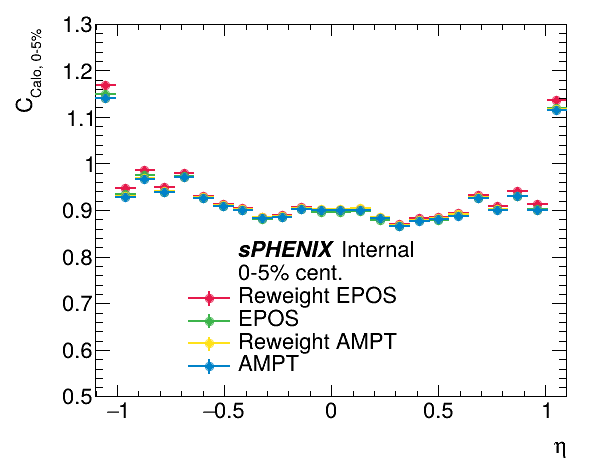
\includegraphics[width=0.24\linewidth]{detdeta/Figures/particle_reweighting_ratios/calo_corr_0-5.png}
    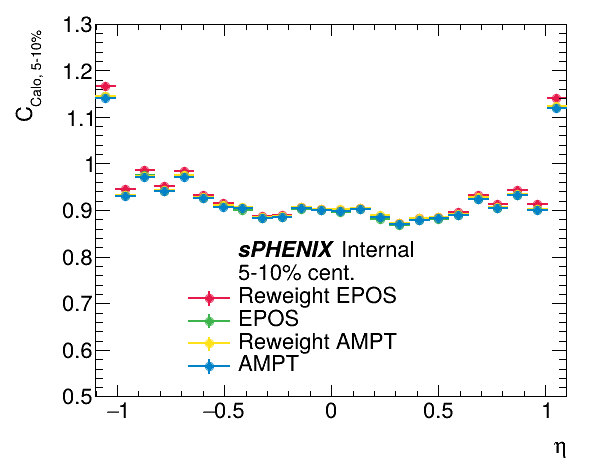
\includegraphics[width=0.24\linewidth]{detdeta/Figures/particle_reweighting_ratios/calo_corr_5-10.png}
    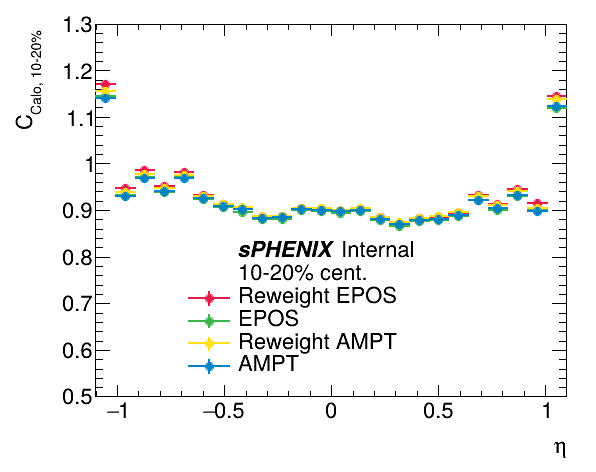
\includegraphics[width=0.24\linewidth]{detdeta/Figures/particle_reweighting_ratios/calo_corr_10-20.png}
    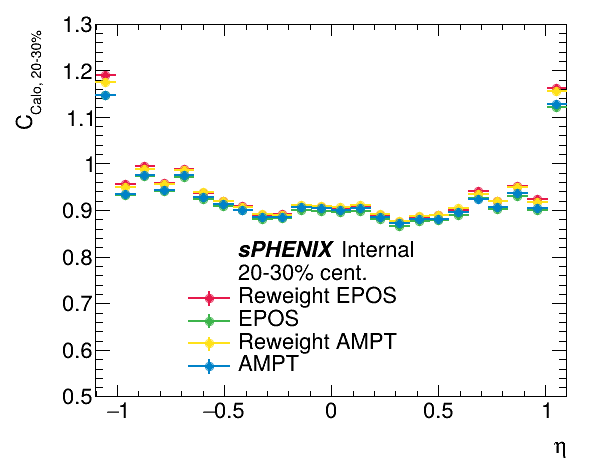
\includegraphics[width=0.24\linewidth]{detdeta/Figures/particle_reweighting_ratios/calo_corr_20-30.png}
    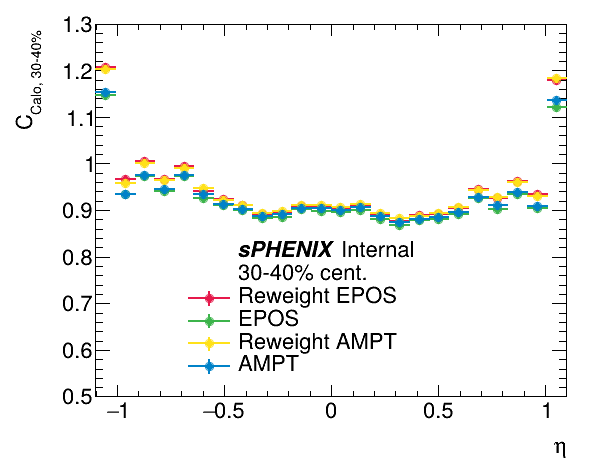
\includegraphics[width=0.24\linewidth]{detdeta/Figures/particle_reweighting_ratios/calo_corr_30-40.png}
    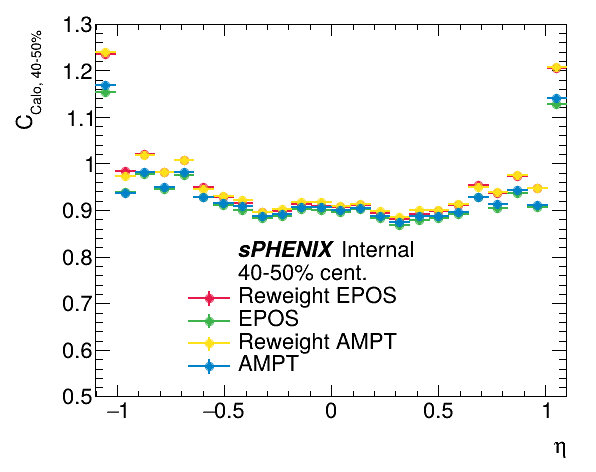
\includegraphics[width=0.24\linewidth]{detdeta/Figures/particle_reweighting_ratios/calo_corr_40-50.png}
    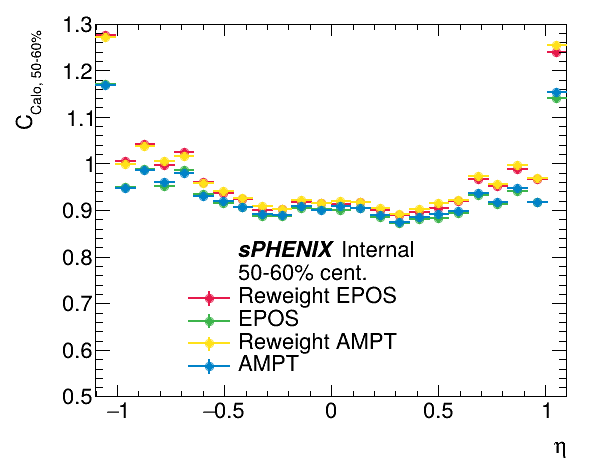
\includegraphics[width=0.24\linewidth]{detdeta/Figures/particle_reweighting_ratios/calo_corr_50-60.png}
    \caption{Effect of reweighting on the correction factors for the EMCal (top), HCal (middle) and full calorimeter for all centrality bins in the analysis.}
    \label{fig:reweighted_corr_factors}
\end{figure}

\begin{figure}
    \centering
    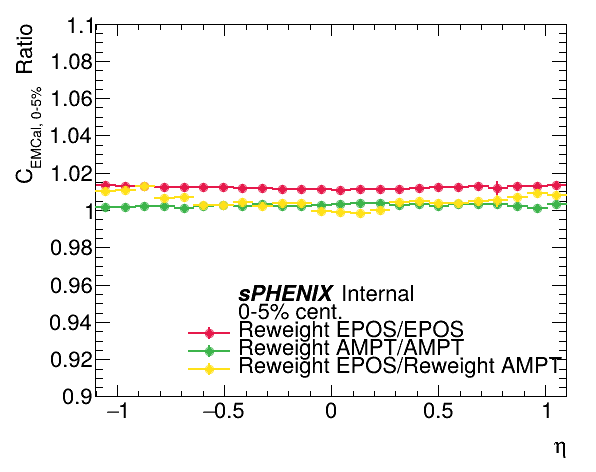
\includegraphics[width=0.24\linewidth]{detdeta/Figures/particle_reweighting_ratios/emcal_ratio_0-5.png}
    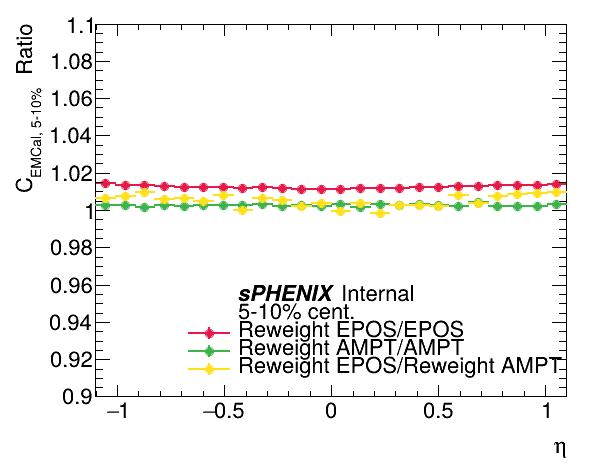
\includegraphics[width=0.24\linewidth]{detdeta/Figures/particle_reweighting_ratios/emcal_ratio_5-10.png}
    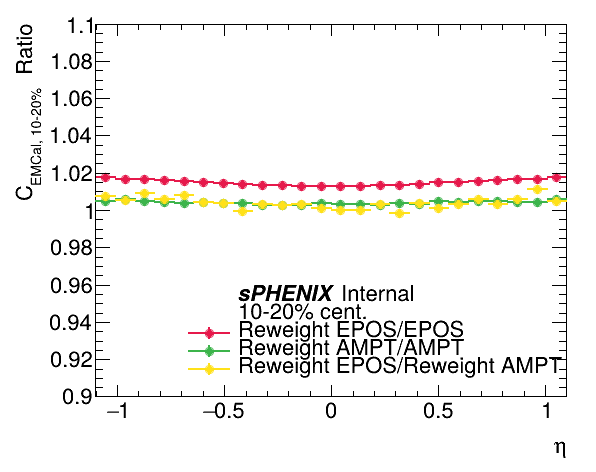
\includegraphics[width=0.24\linewidth]{detdeta/Figures/particle_reweighting_ratios/emcal_ratio_10-20.png}
    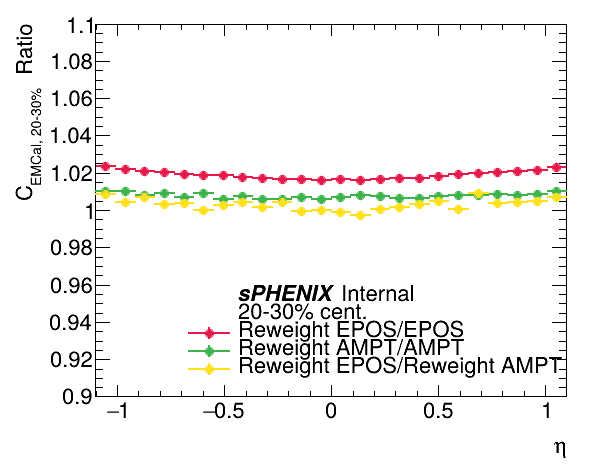
\includegraphics[width=0.24\linewidth]{detdeta/Figures/particle_reweighting_ratios/emcal_ratio_20-30.png}
    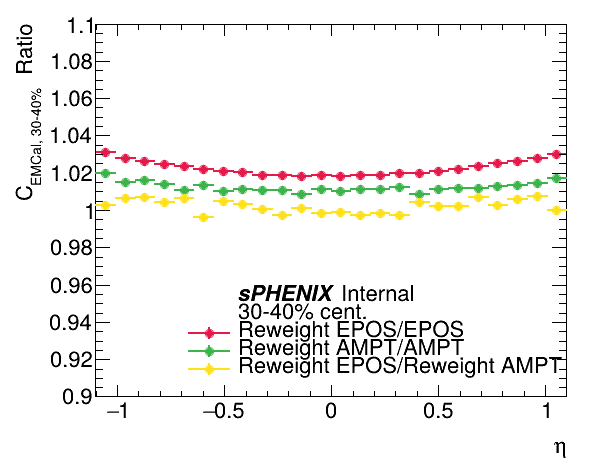
\includegraphics[width=0.24\linewidth]{detdeta/Figures/particle_reweighting_ratios/emcal_ratio_30-40.png}
    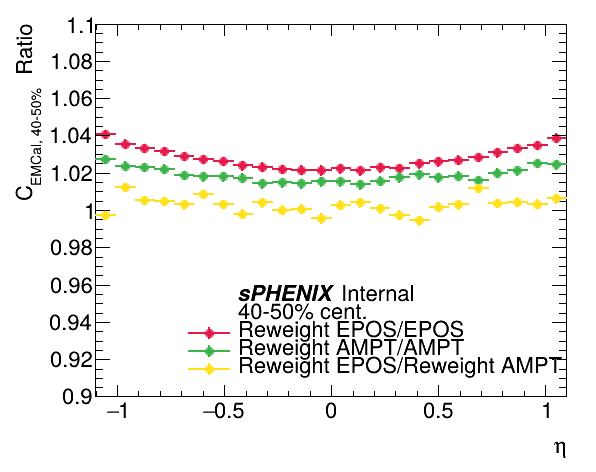
\includegraphics[width=0.24\linewidth]{detdeta/Figures/particle_reweighting_ratios/emcal_ratio_40-50.png}
    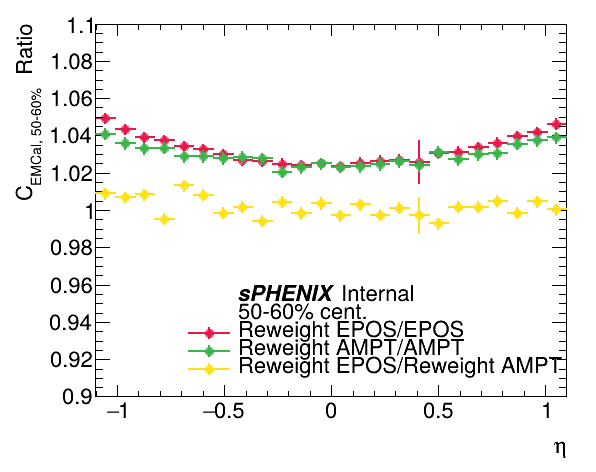
\includegraphics[width=0.24\linewidth]{detdeta/Figures/particle_reweighting_ratios/emcal_ratio_50-60.png} \\
    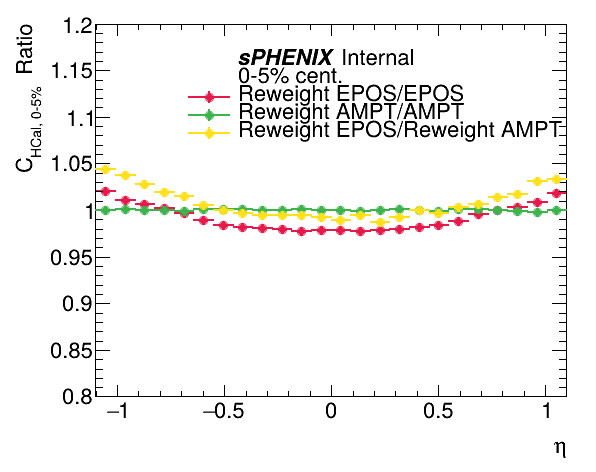
\includegraphics[width=0.24\linewidth]{detdeta/Figures/particle_reweighting_ratios/hcal_ratio_0-5.png}
    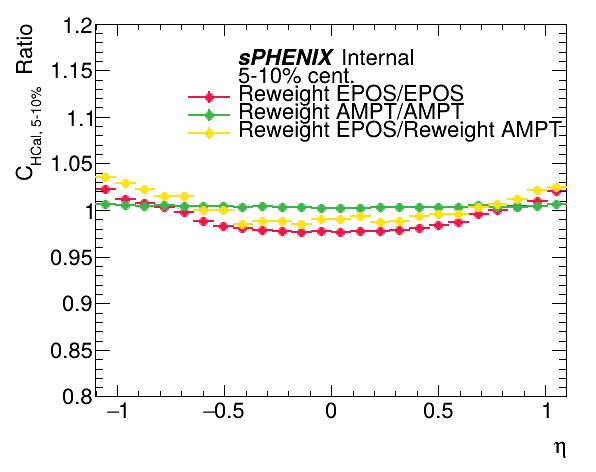
\includegraphics[width=0.24\linewidth]{detdeta/Figures/particle_reweighting_ratios/hcal_ratio_5-10.png}
    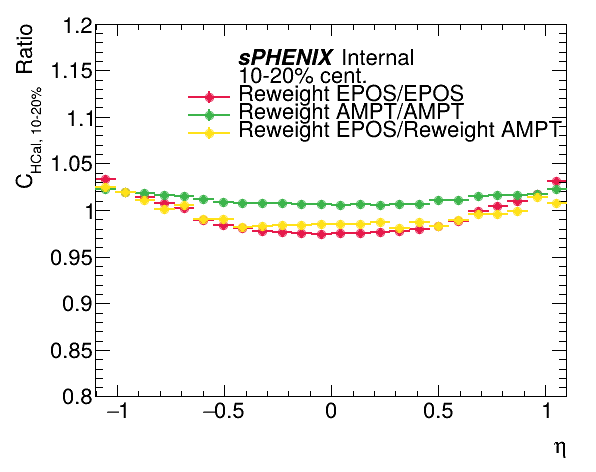
\includegraphics[width=0.24\linewidth]{detdeta/Figures/particle_reweighting_ratios/hcal_ratio_10-20.png}
    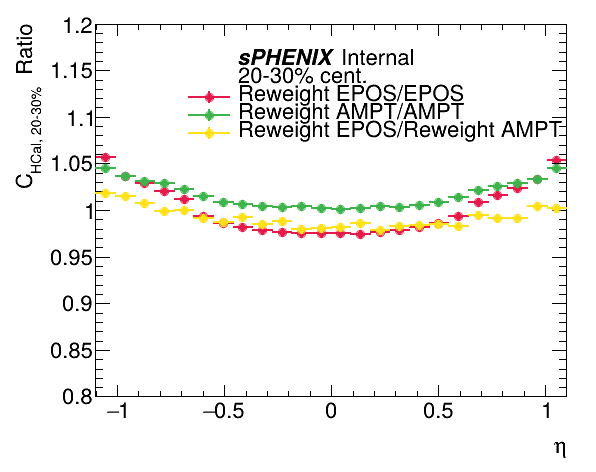
\includegraphics[width=0.24\linewidth]{detdeta/Figures/particle_reweighting_ratios/hcal_ratio_20-30.png}
    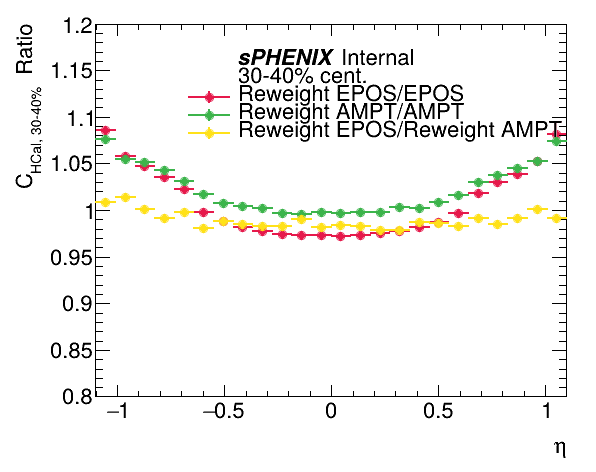
\includegraphics[width=0.24\linewidth]{detdeta/Figures/particle_reweighting_ratios/hcal_ratio_30-40.png}
    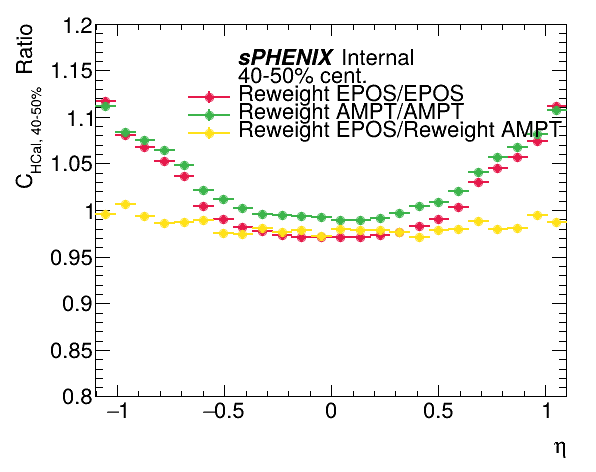
\includegraphics[width=0.24\linewidth]{detdeta/Figures/particle_reweighting_ratios/hcal_ratio_40-50.png}
    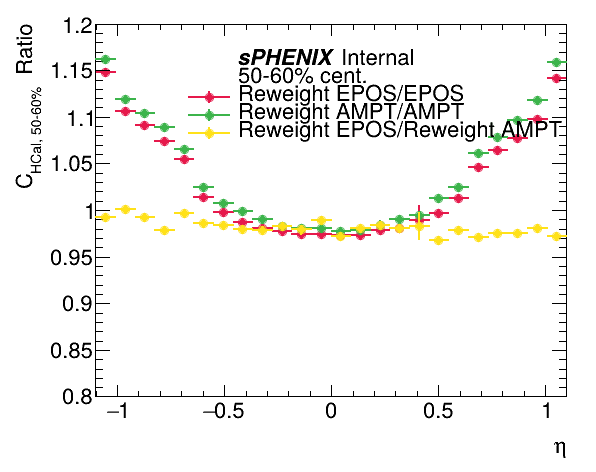
\includegraphics[width=0.24\linewidth]{detdeta/Figures/particle_reweighting_ratios/hcal_ratio_50-60.png} \\
    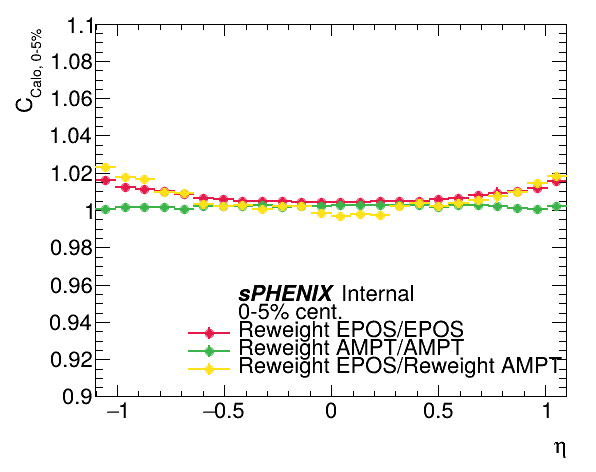
\includegraphics[width=0.24\linewidth]{detdeta/Figures/particle_reweighting_ratios/calo_ratio_0-5.png}
    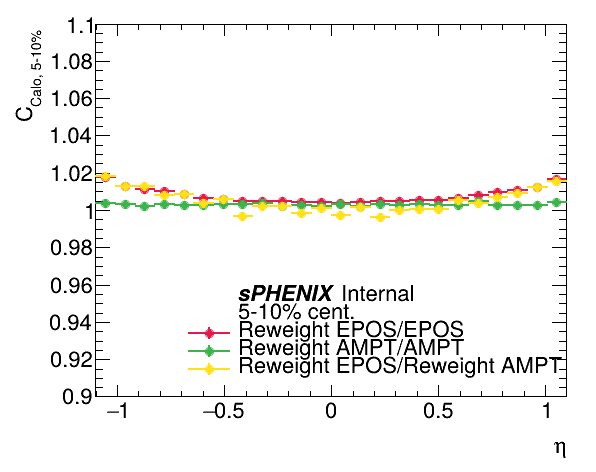
\includegraphics[width=0.24\linewidth]{detdeta/Figures/particle_reweighting_ratios/calo_ratio_5-10.png}
    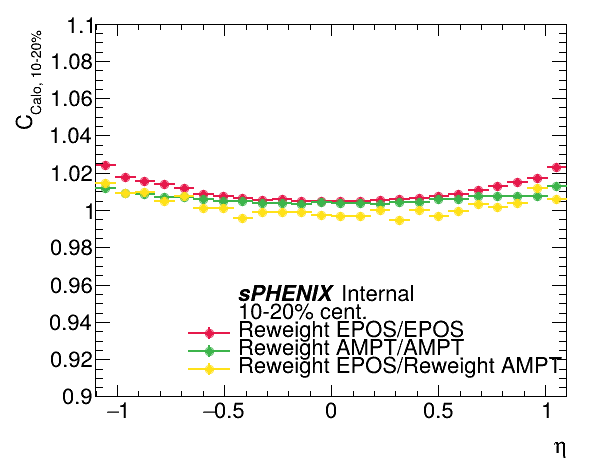
\includegraphics[width=0.24\linewidth]{detdeta/Figures/particle_reweighting_ratios/calo_ratio_10-20.png}
    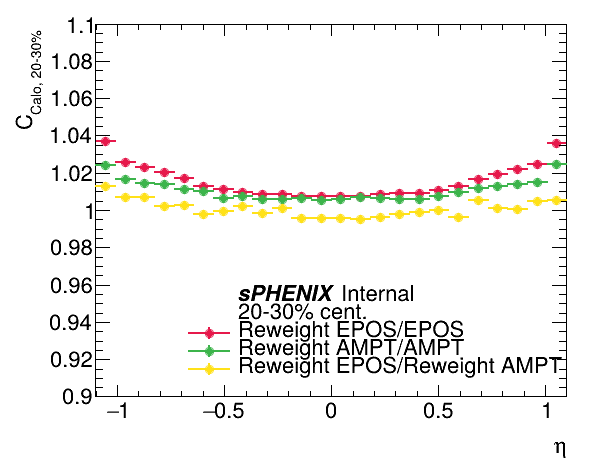
\includegraphics[width=0.24\linewidth]{detdeta/Figures/particle_reweighting_ratios/calo_ratio_20-30.png}
    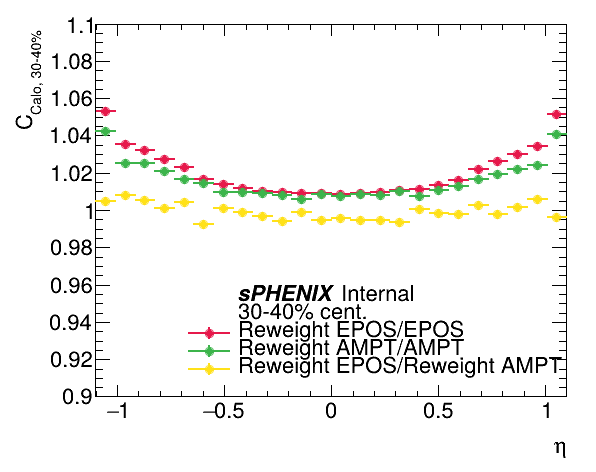
\includegraphics[width=0.24\linewidth]{detdeta/Figures/particle_reweighting_ratios/calo_ratio_30-40.png}
    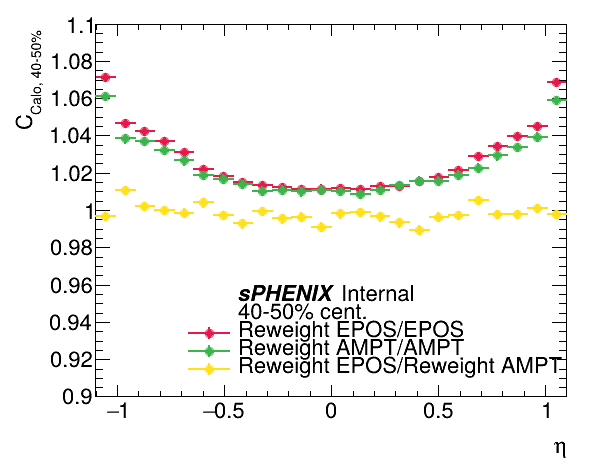
\includegraphics[width=0.24\linewidth]{detdeta/Figures/particle_reweighting_ratios/calo_ratio_40-50.png}
    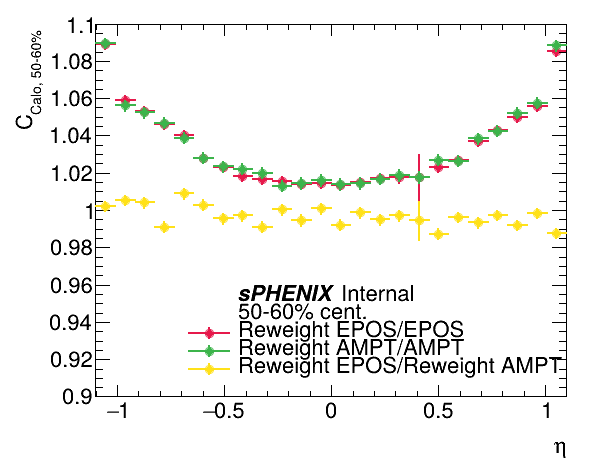
\includegraphics[width=0.24\linewidth]{detdeta/Figures/particle_reweighting_ratios/calo_ratio_50-60.png}
    \caption{Ratio of correction factors with and without the particle reweighting applied for the EMCal (top) and HCal (bottom) for all centrality bins in the analysis.}
    \label{fig:reweighted_corr_ratio}
\end{figure} 

\chapter{HCal Sampling Fraction Studies}
\label{sec:SamplingFrac}
\input{detdeta_hcal_sampling_fraction}

\chapter{Simulation of Support Structures}
\label{sec:SupportStruct}
The effect of including the sPHENIX support structures in the simulation, namely the sPHENIX magnet pole tip doors and IHCal support structure ring, are studied by comparing the reconstructed level \detdeta results from data to that from simulation with and without these support structures simulated. 
The reconstruction level \detdeta for the IHCal-only and OHCal-only measurements are shown in Figure \ref{fig:hcal_pole_tip_door_comparison}. 
Here a comparison between the reconstructed level \detdeta from data and EPOS simulation with and without pole tip doors simulated is shown.
The simulation with pole tip doors on better reproduces the shape of the HCal detector response seen in data, particularly in the wings of the \detdeta distribution ($|\eta| < 0.5$ in OHCal and $|\eta| < 0.8$ in IHCal).

\begin{figure}
    \centering
    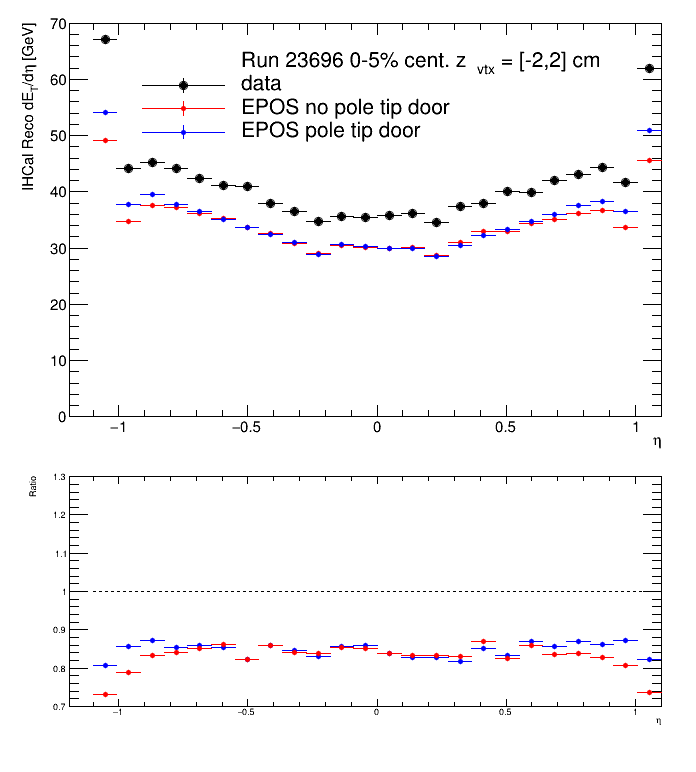
\includegraphics[width=0.48\linewidth]{detdeta/Figures/pole_tip_doors/ihcal_reco_0-5_epos_plugdoor_z=0_wratio.png}
    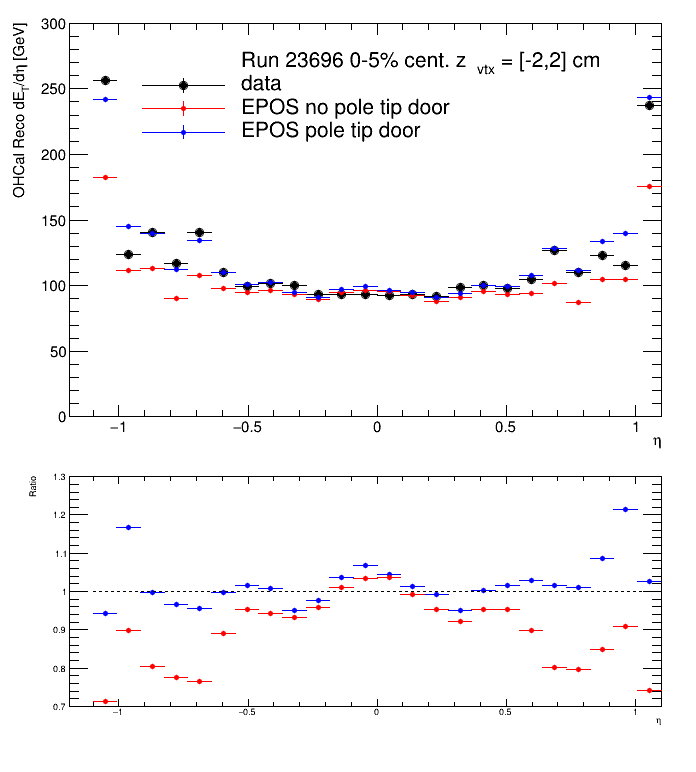
\includegraphics[width=0.48\linewidth]{detdeta/Figures/pole_tip_doors/ohcal_reco_0-5_epos_plugdoor_z=0_wratio.png}
    \caption{Plots made with ana.389p004 and privately generated EPOS simualtion (with timing bug)}
    \label{fig:hcal_pole_tip_door_comparison}
\end{figure}

In Figure \ref{fig:hcal_pole_tip_door_comparison}, there is still a remaining disagreement between the data and simulation OHCal detector response seen at $|\eta| ~ 1$ in the OHCal \detdeta distribution.
Investigation into the engineering documents of the the IHCal support structure revealed that there are support ring components mounted on the face of the towers in the OHCal at $|\eta| ~ 1$ which were not included in the simulation.
The simulation was updated to include these support ring components and the \detdeta result from simulation correction factors with and without these support ring components were compared.
Figure \ref{fig:ihcal_support_structure_comparison} shows the comparison of the fully corrected \detdeta results using correction factors which does not have the support ring geometry included (labeled "HIJING run 101") and which does have the support ring geometry included (labeled "HIJING run 14").
The discontinuity originally seen in the OHCal \detdeta measurement at $|\eta|$ = 1.0 is no longer present in the OHCal \detdeta measurement when using correction factors from the simulation with the support ring geometry included.

\begin{figure}
    \centering
    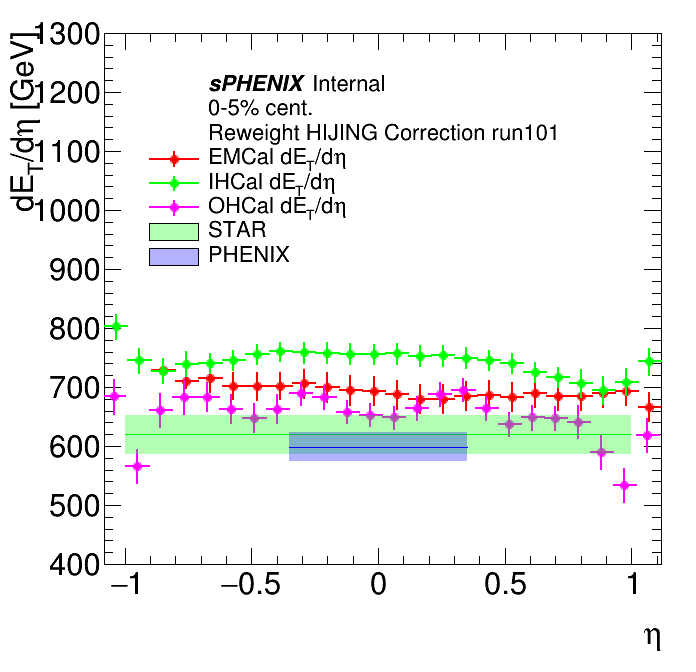
\includegraphics[width=0.48\linewidth]{detdeta/Figures/ihcal_support_structure/detdeta_reweight_hijing_run101_0-5.png}
    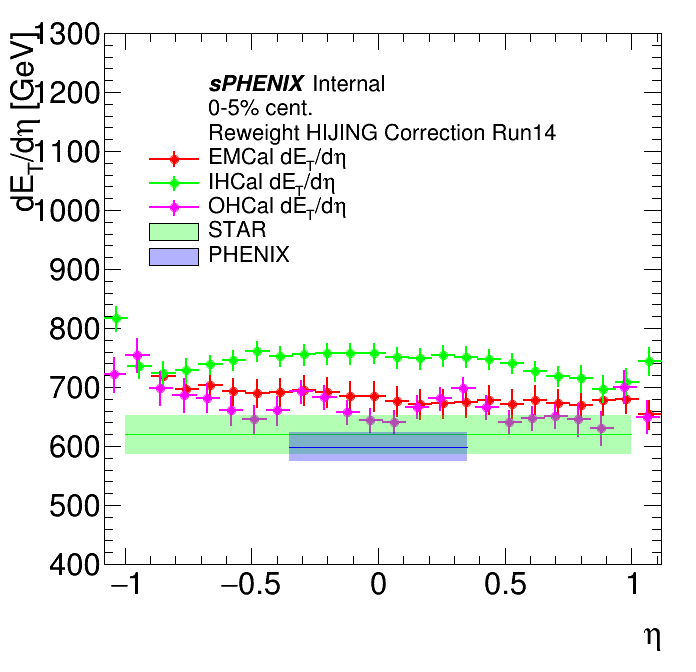
\includegraphics[width=0.48\linewidth]{detdeta/Figures/ihcal_support_structure/detdeta_reweight_hijing_run14_0-5.png}
    \caption{Comparison of fully corrected \detdeta measurements using correction factors from HIJING run 101 (left) and HIJING run 14 (right). The OHCal \detdeta measurement at $|\eta|$ = 1.0 dips in the HIJING run 101 plot due to data and MC geometry mismatch is rectified in the OHCal \detdeta measurement in the HIJING run 101 plot.}
    \label{fig:ihcal_support_structure_comparison}
\end{figure}

\chapter{Full \detdeta Plots for All Centrality Bins}
\label{sec:full_detdeta_plots}
\input{detdeta_full_plots}

\chapter{Additional \detdeta Systematics Results}
\label{sec:detdeta_add_syst}
Presented in this section are additional results on the systematic variations for the \detdeta measurement. 
The metholodogy for producing these results is described in detail in Section~\ref{sec:detdeta_systematics}.
However, only a selection of example systematic plots are included in the main body for brevity. 
Figures~\ref{fig:eta_dep_syst_ihcal} and \ref{fig:eta_dep_syst_ohcal} show the contributions from all systematic variations in the analysis on the IHCal-only and OHCal-only measurements of \detdeta as a function of $\eta$.

\begin{figure}
    \centering
    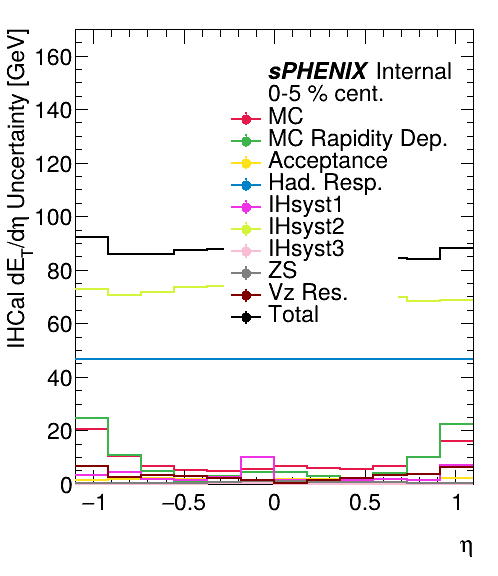
\includegraphics[width=0.32\linewidth]{figures/chapter4/ihcal_total_syst_0-5.png}
    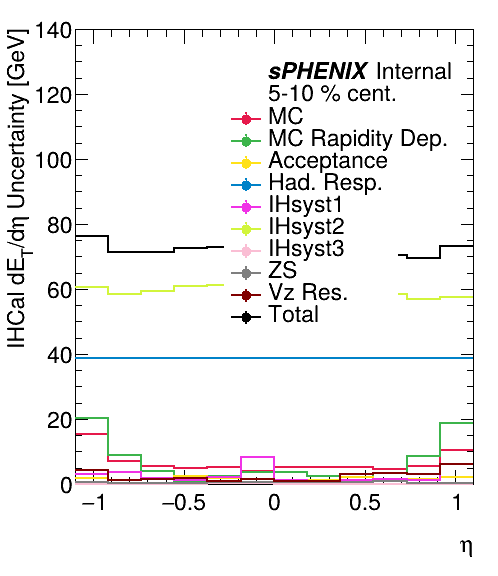
\includegraphics[width=0.32\linewidth]{figures/chapter4/ihcal_total_syst_5-10.png}
    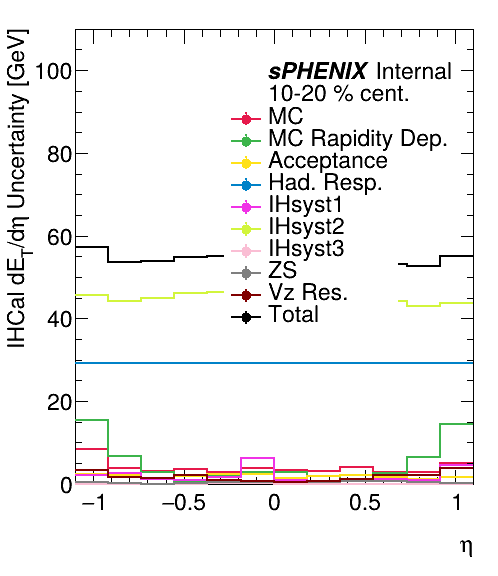
\includegraphics[width=0.32\linewidth]{figures/chapter4/ihcal_total_syst_10-20.png}
    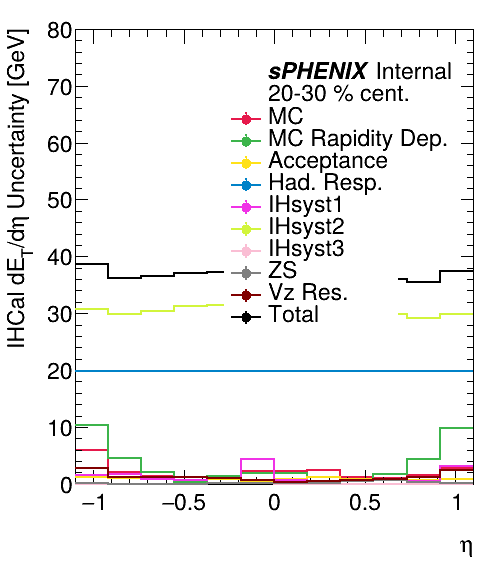
\includegraphics[width=0.32\linewidth]{figures/chapter4/ihcal_total_syst_20-30.png}
    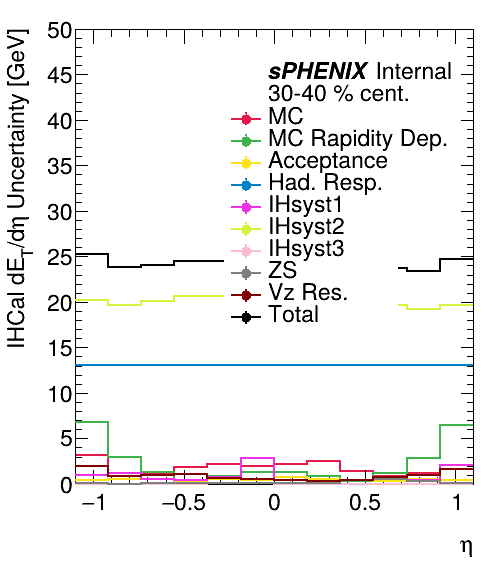
\includegraphics[width=0.32\linewidth]{figures/chapter4/ihcal_total_syst_30-40.png}
    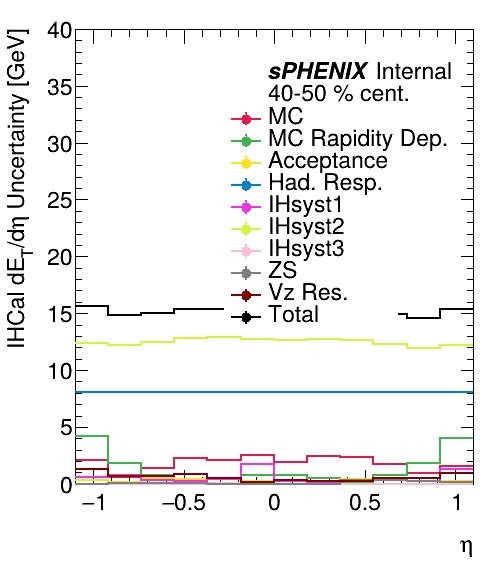
\includegraphics[width=0.32\linewidth]{figures/chapter4/ihcal_total_syst_40-50.png}
    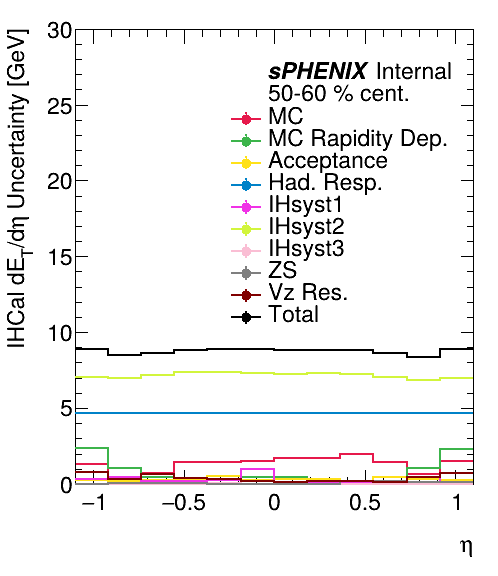
\includegraphics[width=0.32\linewidth]{figures/chapter4/ihcal_total_syst_50-60.png}
    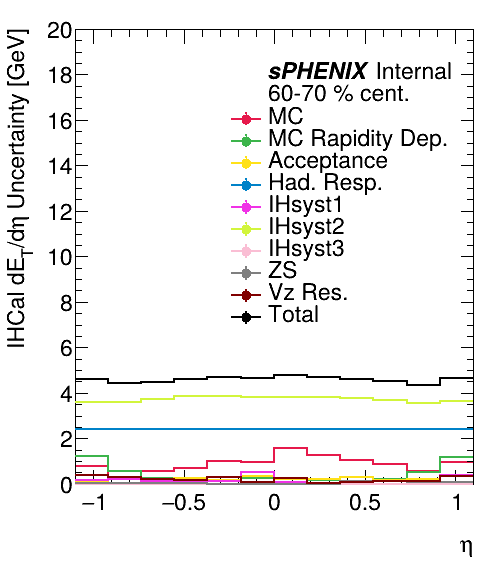
\includegraphics[width=0.32\linewidth]{figures/chapter4/ihcal_total_syst_60-70.png}
    \caption{Systematic uncertainties on \detdeta measurements as a function of $\eta$ for \detdeta measurements from IHCal-only data. Uncertainties from all centralities in measurement are shown in increasing order from top to bottom.}
    \label{fig:eta_dep_syst_ihcal}
\end{figure}

\begin{figure}
    \centering
    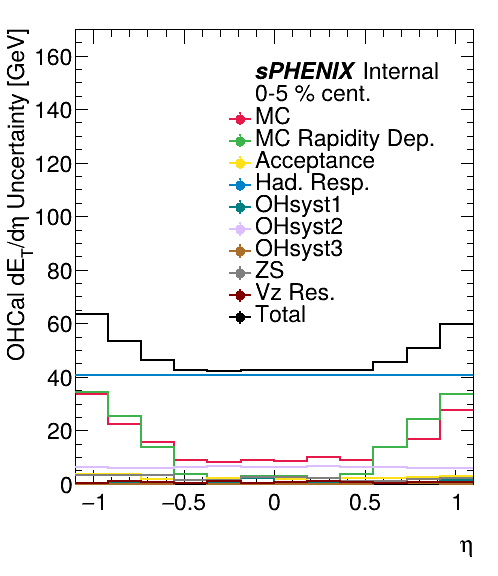
\includegraphics[width=0.32\linewidth]{figures/chapter4/ohcal_total_syst_0-5.png}
    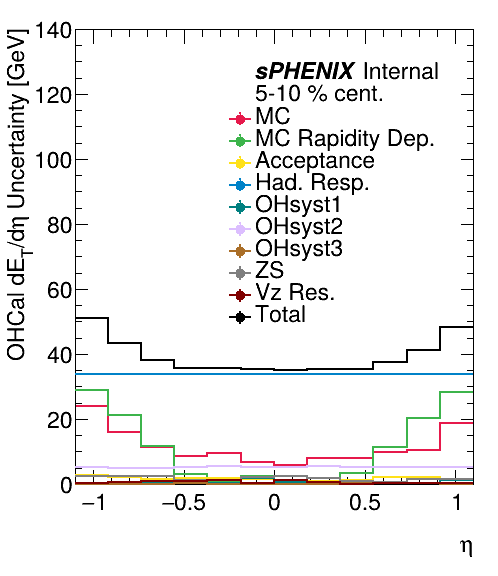
\includegraphics[width=0.32\linewidth]{figures/chapter4/ohcal_total_syst_5-10.png}
    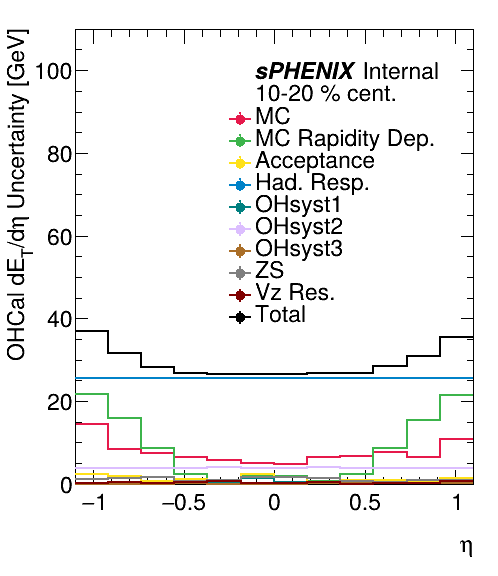
\includegraphics[width=0.32\linewidth]{figures/chapter4/ohcal_total_syst_10-20.png}
    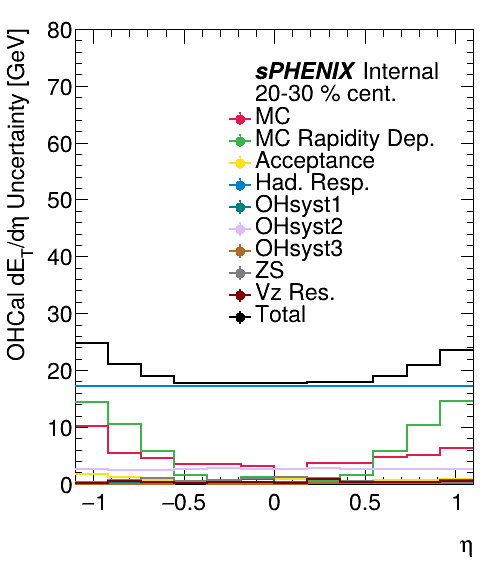
\includegraphics[width=0.32\linewidth]{figures/chapter4/ohcal_total_syst_20-30.png}
    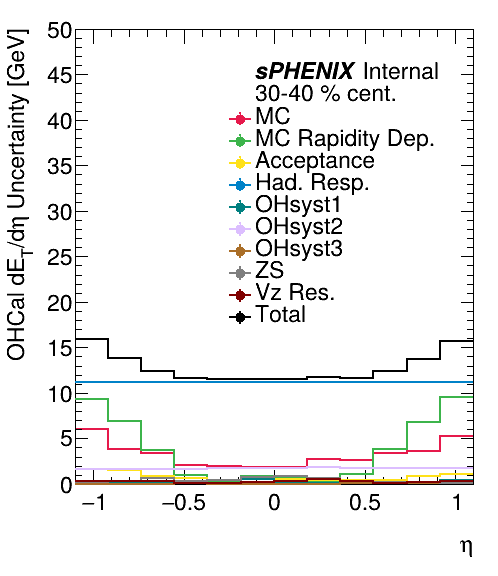
\includegraphics[width=0.32\linewidth]{figures/chapter4/ohcal_total_syst_30-40.png}
    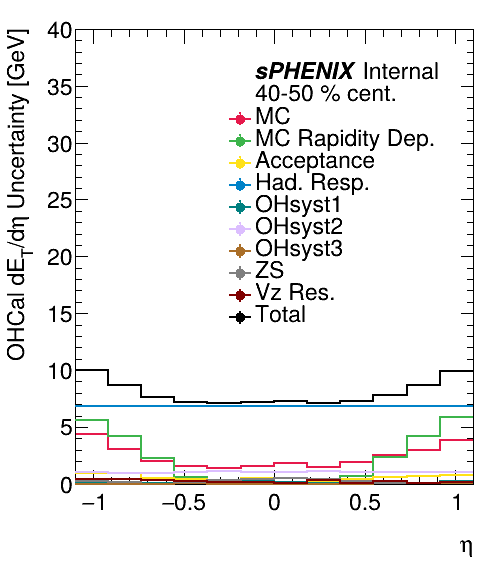
\includegraphics[width=0.32\linewidth]{figures/chapter4/ohcal_total_syst_40-50.png}
    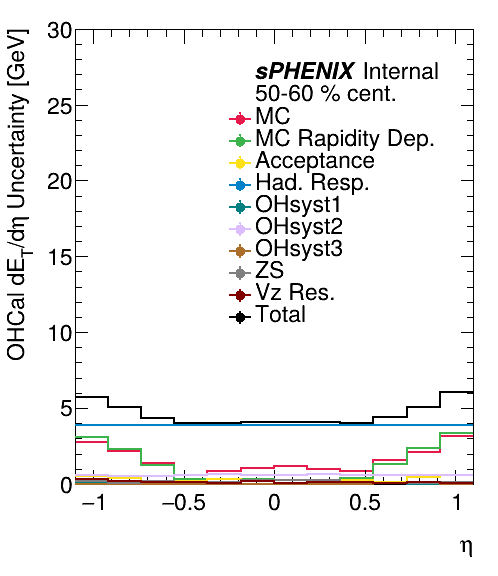
\includegraphics[width=0.32\linewidth]{figures/chapter4/ohcal_total_syst_50-60.png}
    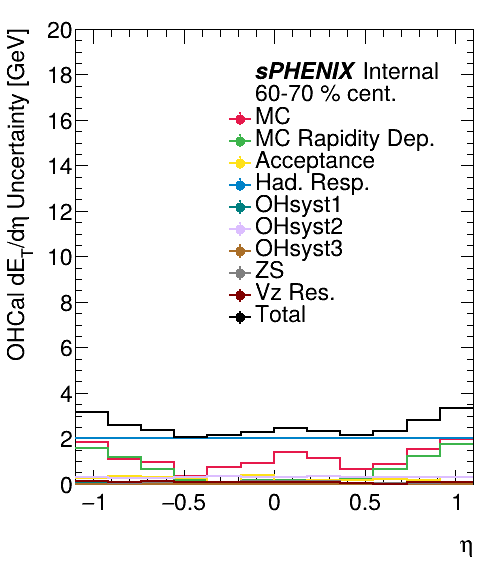
\includegraphics[width=0.32\linewidth]{figures/chapter4/ohcal_total_syst_60-70.png}
    \caption{Systematic uncertainties on \detdeta measurements as a function of $\eta$ for \detdeta measurements from OHCal-only data. Uncertainties from all centralities in measurement are shown in increasing order from top to bottom.}
    \label{fig:eta_dep_syst_ohcal}
\end{figure}

The metholodogy for determining the correlation between \detdeta measurements and finding the agreement between measurements within uncorrelated uncertainties is also outlined in Section~\ref{sec:detdeta_systematics}.
Additional scatter plots for determining the correlation between the positive and negative $\eta$ measurements of \detdeta using only EMCal or HCal data are included in Figures~\ref{fig:emcal_eta_covariance} and \ref{fig:hcal_eta_covariance}.
Finally, the ratio of measurements of \detdeta at positive and negative $\eta$ using only the EMCal or HCal data are included in Figures~\ref{fig:emcal_eta_detdeta_ratio} and \ref{fig:hcal_eta_detdeta_ratio}.

\begin{figure}
    \centering
    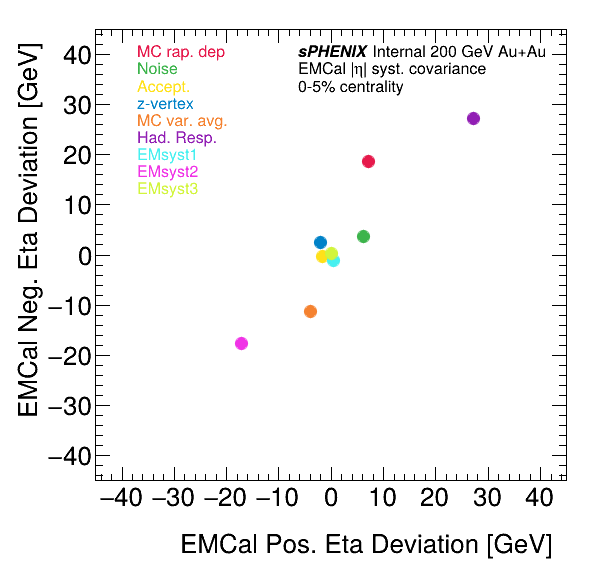
\includegraphics[width=0.32\linewidth]{detdeta/Figures/corr_syst_uncertainties/emcal_pos_neg_eta_covariance_0-5.png}
    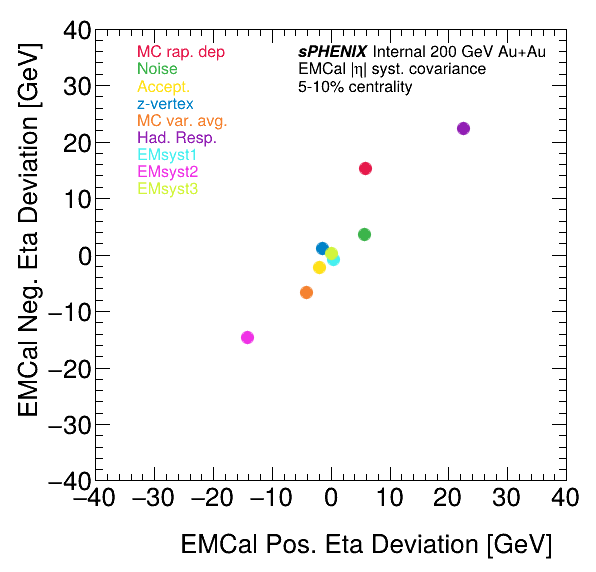
\includegraphics[width=0.32\linewidth]{detdeta/Figures/corr_syst_uncertainties/emcal_pos_neg_eta_covariance_5-10.png}
    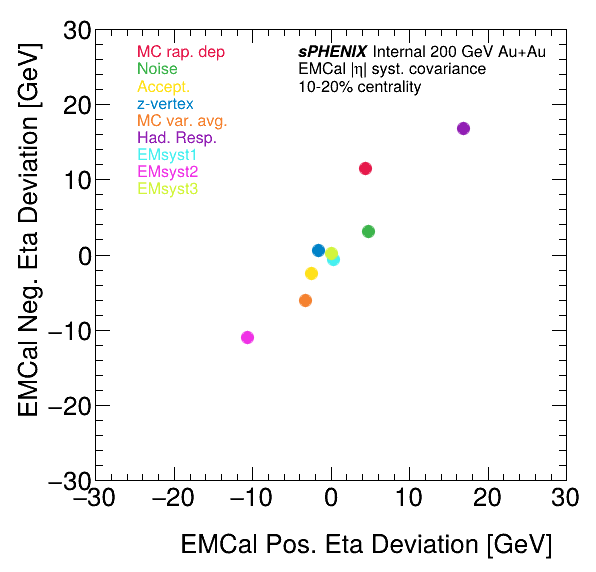
\includegraphics[width=0.32\linewidth]{detdeta/Figures/corr_syst_uncertainties/emcal_pos_neg_eta_covariance_10-20.png}
    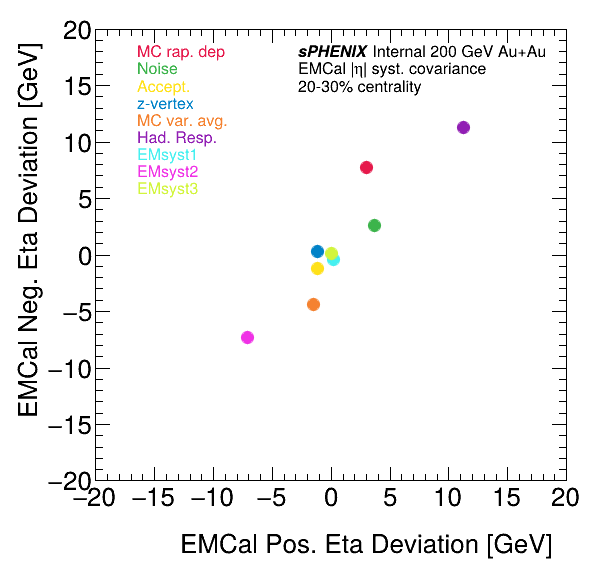
\includegraphics[width=0.32\linewidth]{detdeta/Figures/corr_syst_uncertainties/emcal_pos_neg_eta_covariance_20-30.png}
    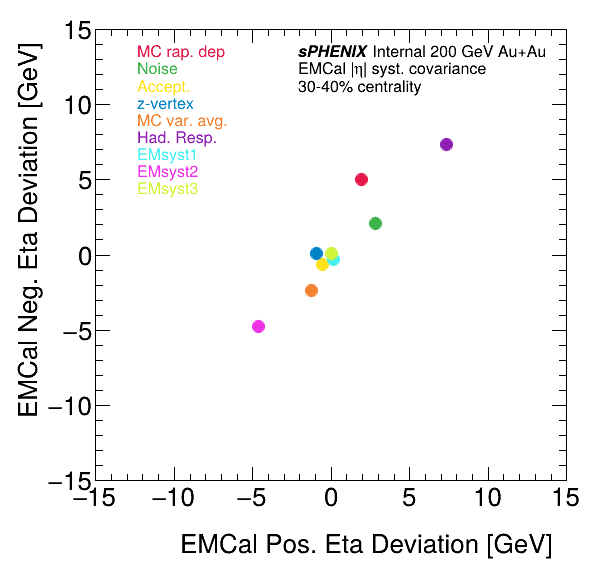
\includegraphics[width=0.32\linewidth]{detdeta/Figures/corr_syst_uncertainties/emcal_pos_neg_eta_covariance_30-40.png}
    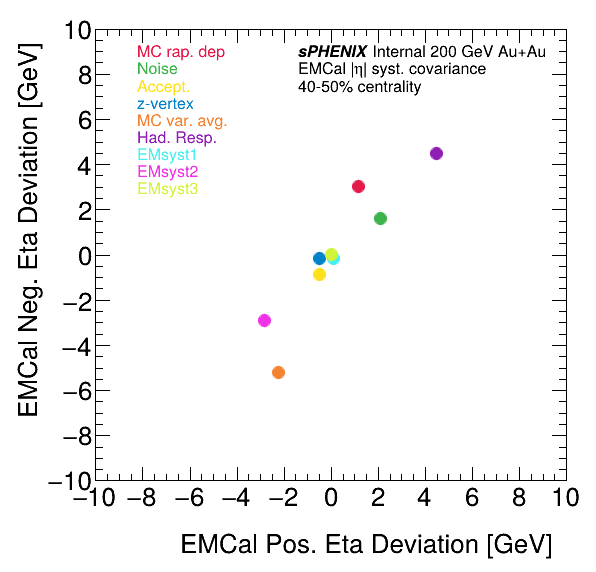
\includegraphics[width=0.32\linewidth]{detdeta/Figures/corr_syst_uncertainties/emcal_pos_neg_eta_covariance_40-50.png}
    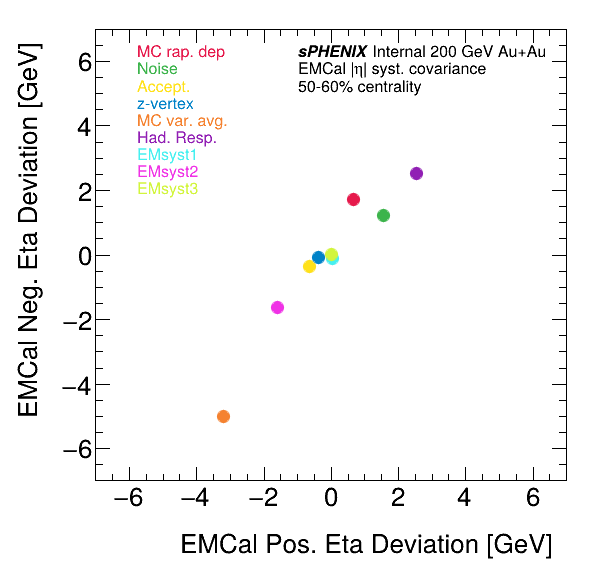
\includegraphics[width=0.32\linewidth]{detdeta/Figures/corr_syst_uncertainties/emcal_pos_neg_eta_covariance_50-60.png}
    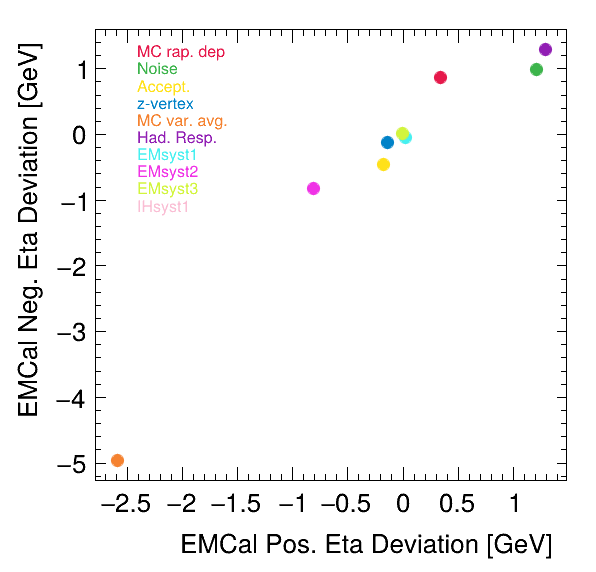
\includegraphics[width=0.32\linewidth]{figures/chapter4/emcal_pos_neg_eta_covariance_prc_edit_60-70.png}
    \caption{Correlation plots for the EMCal \detdeta measurements at $0.74 < |\eta| < 1.1$ using each analysis systematic variation for each centrality measurement in the analysis.}
    \label{fig:emcal_eta_covariance}
\end{figure}
\begin{figure}
    \centering
    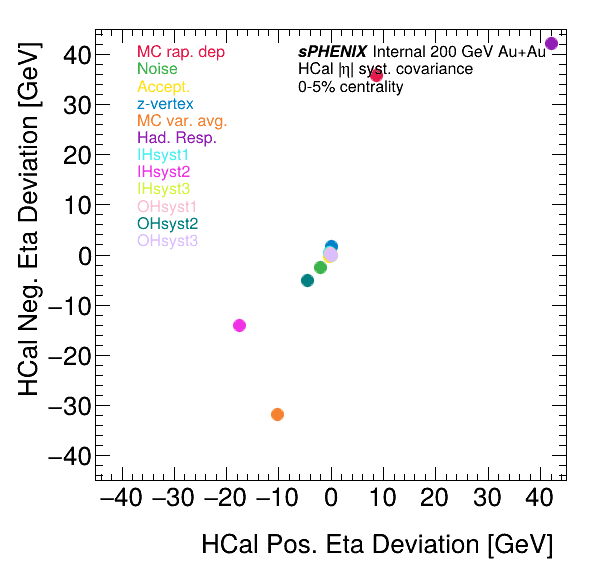
\includegraphics[width=0.32\linewidth]{detdeta/Figures/corr_syst_uncertainties/hcal_pos_neg_eta_covariance_0-5.png}
    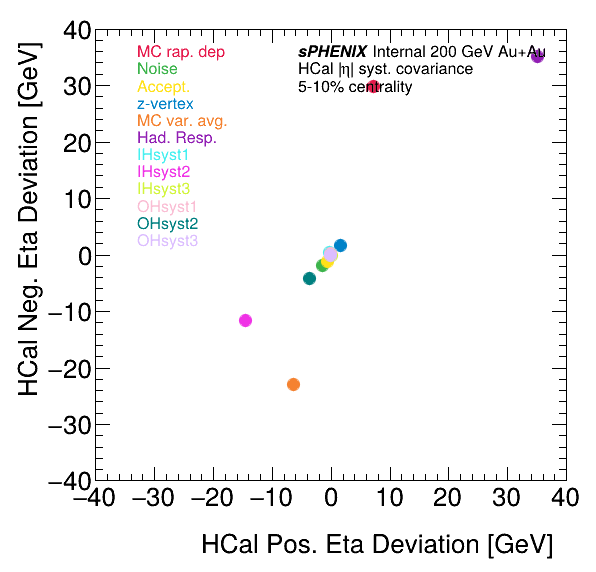
\includegraphics[width=0.32\linewidth]{detdeta/Figures/corr_syst_uncertainties/hcal_pos_neg_eta_covariance_5-10.png}
    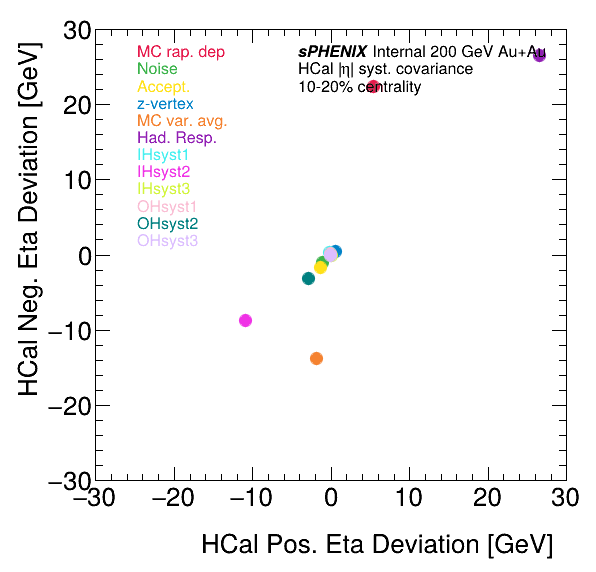
\includegraphics[width=0.32\linewidth]{detdeta/Figures/corr_syst_uncertainties/hcal_pos_neg_eta_covariance_10-20.png}
    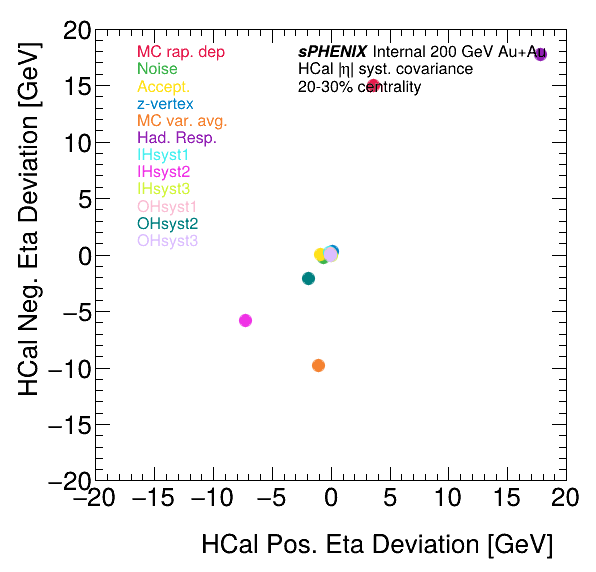
\includegraphics[width=0.32\linewidth]{detdeta/Figures/corr_syst_uncertainties/hcal_pos_neg_eta_covariance_20-30.png}
    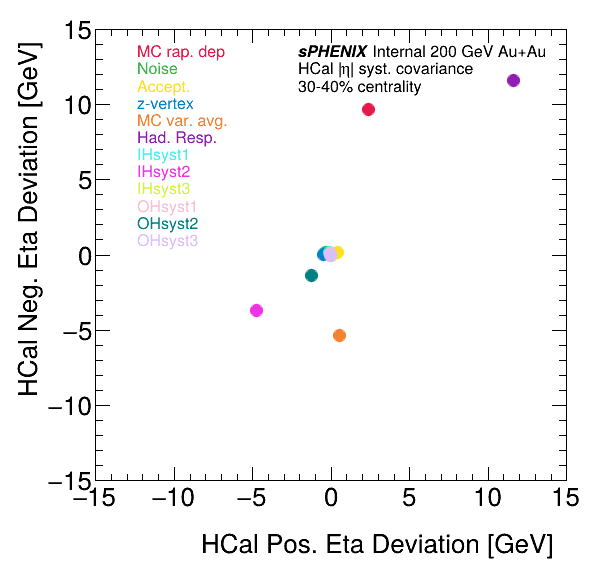
\includegraphics[width=0.32\linewidth]{detdeta/Figures/corr_syst_uncertainties/hcal_pos_neg_eta_covariance_30-40.png}
    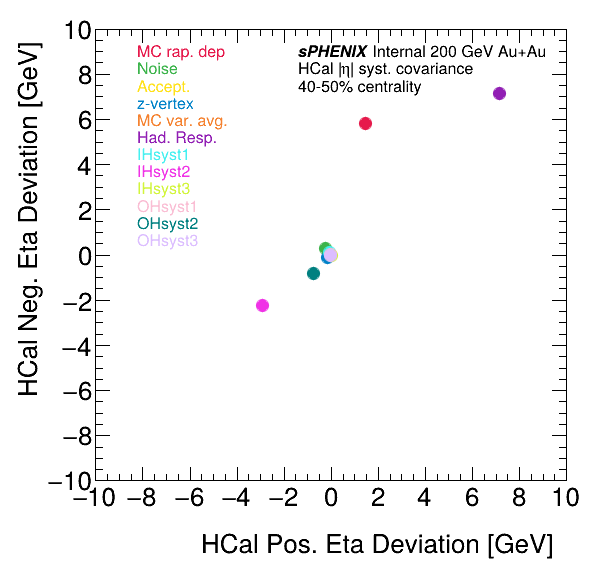
\includegraphics[width=0.32\linewidth]{detdeta/Figures/corr_syst_uncertainties/hcal_pos_neg_eta_covariance_40-50.png}
    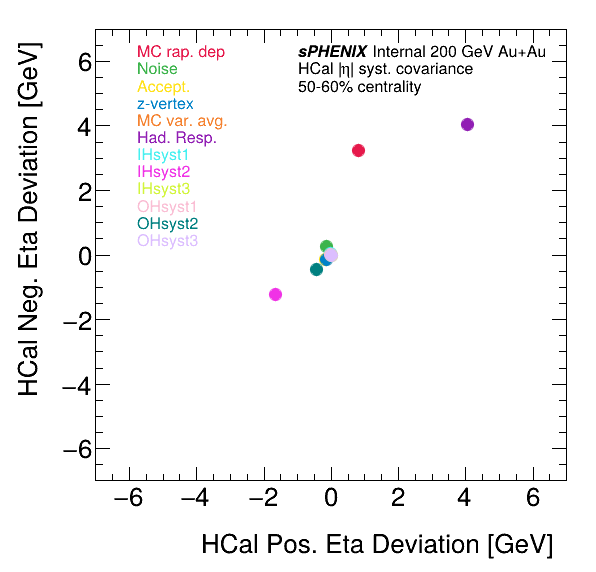
\includegraphics[width=0.32\linewidth]{detdeta/Figures/corr_syst_uncertainties/hcal_pos_neg_eta_covariance_50-60.png}
    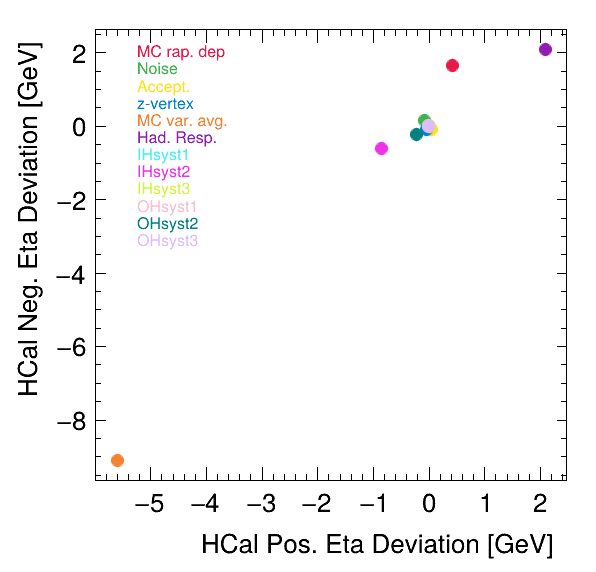
\includegraphics[width=0.32\linewidth]{figures/chapter4/hcal_pos_neg_eta_covariance_prc_edit_60-70.png}
    \caption{Correlation plots for the HCal \detdeta measurements at $0.74 < |\eta| < 1.1$ using each analysis systematic variation for each centrality measurement in the analysis.}
    \label{fig:hcal_eta_covariance}
\end{figure}

\begin{figure}
    \centering
    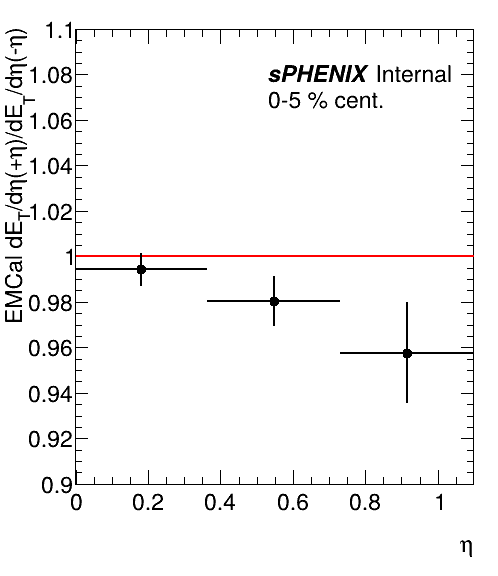
\includegraphics[width=0.32\linewidth]{detdeta/Figures/corr_syst_uncertainties/emcal_eta_ratio_syst_0-5.png}
    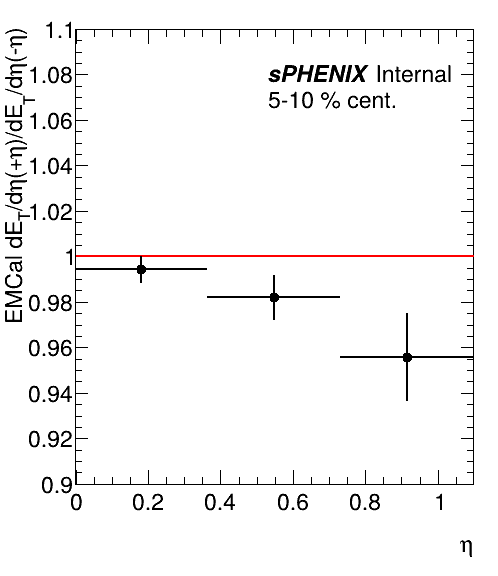
\includegraphics[width=0.32\linewidth]{detdeta/Figures/corr_syst_uncertainties/emcal_eta_ratio_syst_5-10.png}
    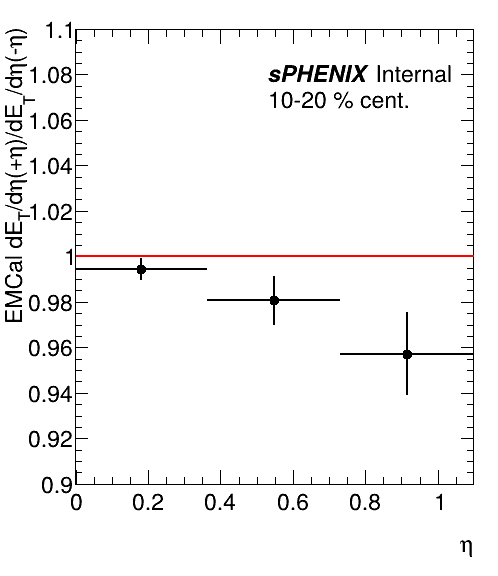
\includegraphics[width=0.32\linewidth]{detdeta/Figures/corr_syst_uncertainties/emcal_eta_ratio_syst_10-20.png}
    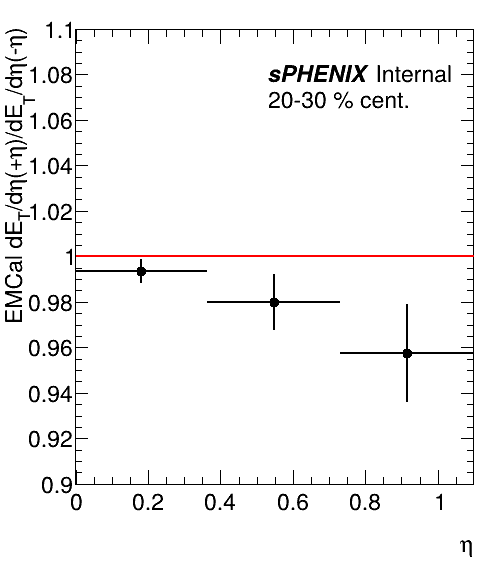
\includegraphics[width=0.32\linewidth]{detdeta/Figures/corr_syst_uncertainties/emcal_eta_ratio_syst_20-30.png}
    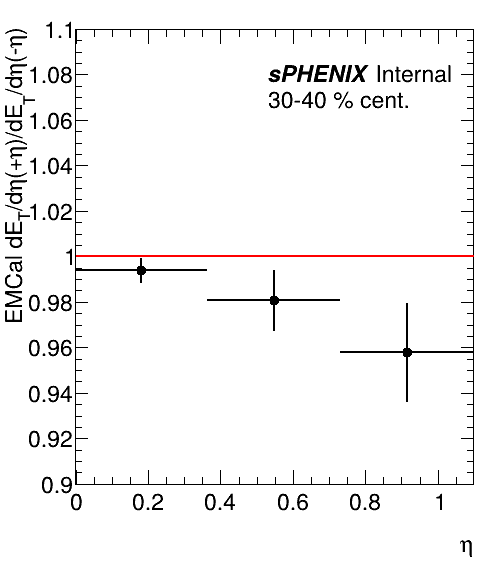
\includegraphics[width=0.32\linewidth]{detdeta/Figures/corr_syst_uncertainties/emcal_eta_ratio_syst_30-40.png}
    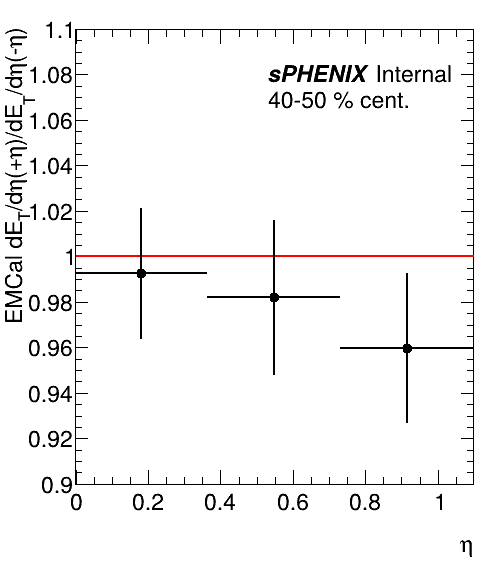
\includegraphics[width=0.32\linewidth]{detdeta/Figures/corr_syst_uncertainties/emcal_eta_ratio_syst_40-50.png}
    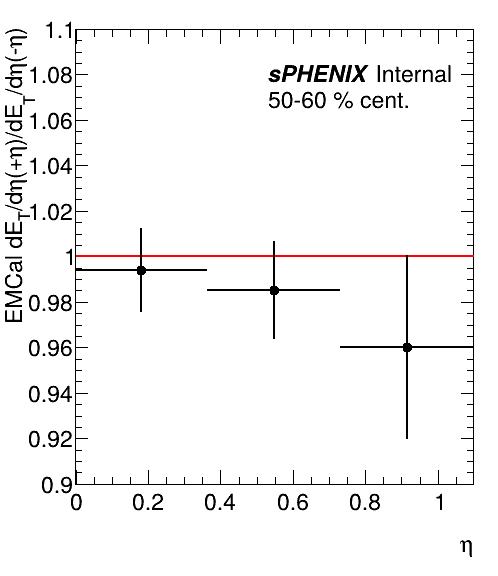
\includegraphics[width=0.32\linewidth]{detdeta/Figures/corr_syst_uncertainties/emcal_eta_ratio_syst_50-60.png}
    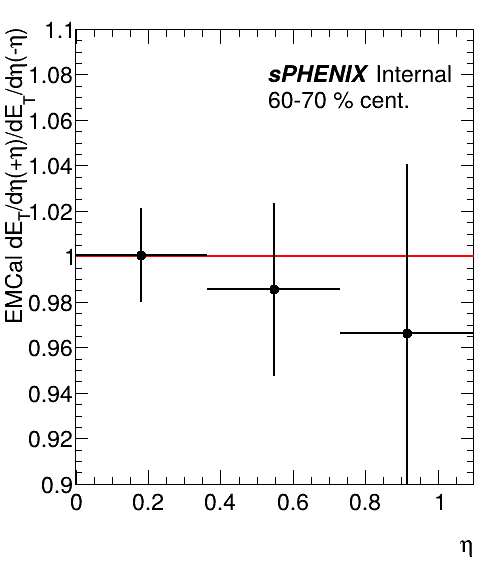
\includegraphics[width=0.32\linewidth]{figures/chapter4/emcal_eta_ratio_syst_60-70.png}
    \caption{Correlation plots for the EMCal \detdeta measurements at $0.74 < |\eta| < 1.1$ using each analysis systematic variation for each centrality measurement in the analysis.}
    \label{fig:emcal_eta_detdeta_ratio}
\end{figure}
\begin{figure}
    \centering
    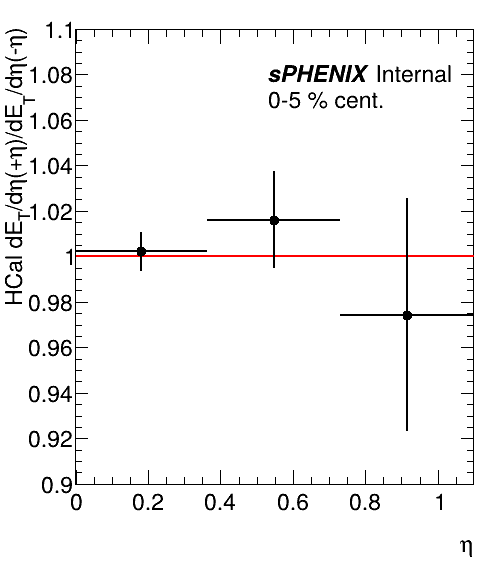
\includegraphics[width=0.32\linewidth] {detdeta/Figures/corr_syst_uncertainties/hcal_eta_ratio_syst_0-5.png}
    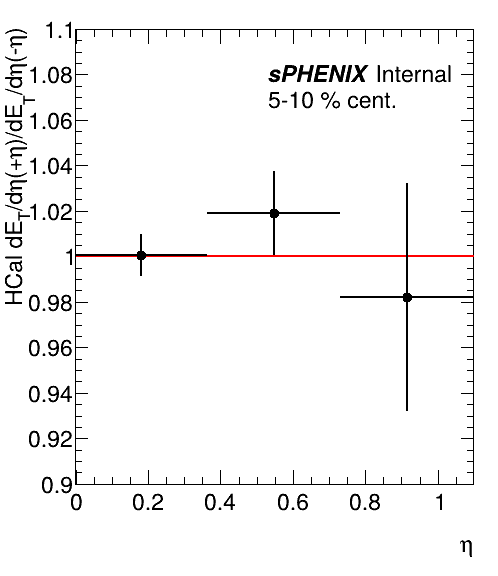
\includegraphics[width=0.32\linewidth]{detdeta/Figures/corr_syst_uncertainties/hcal_eta_ratio_syst_5-10.png}
    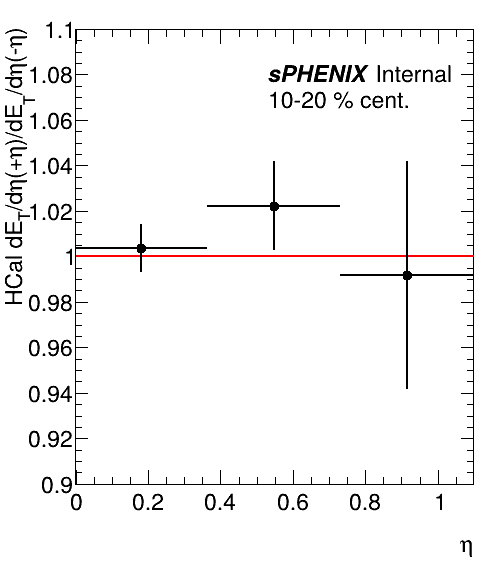
\includegraphics[width=0.32\linewidth]{detdeta/Figures/corr_syst_uncertainties/hcal_eta_ratio_syst_10-20.png}
    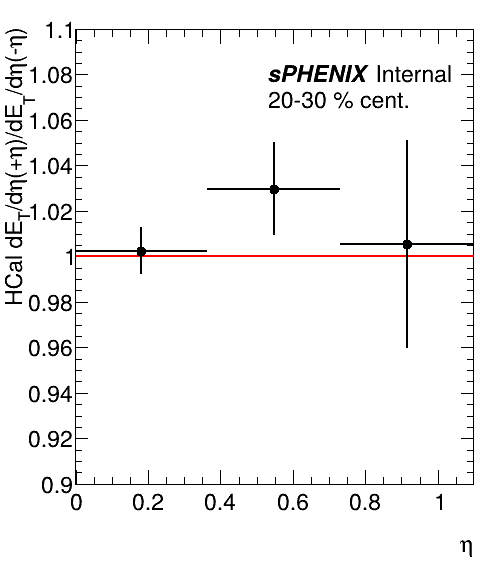
\includegraphics[width=0.32\linewidth]{detdeta/Figures/corr_syst_uncertainties/hcal_eta_ratio_syst_20-30.png}
    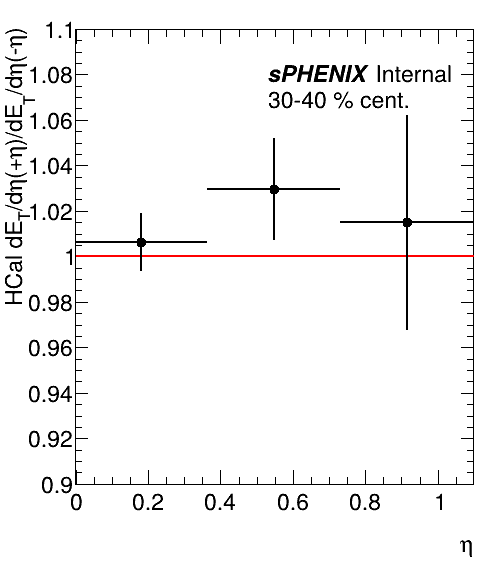
\includegraphics[width=0.32\linewidth]{detdeta/Figures/corr_syst_uncertainties/hcal_eta_ratio_syst_30-40.png}
    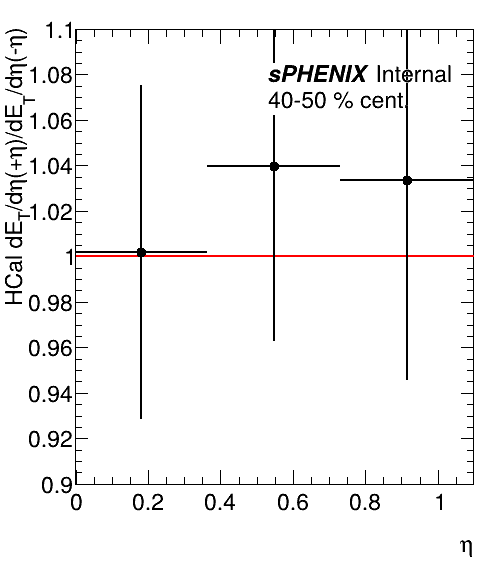
\includegraphics[width=0.32\linewidth]{detdeta/Figures/corr_syst_uncertainties/hcal_eta_ratio_syst_40-50.png}
    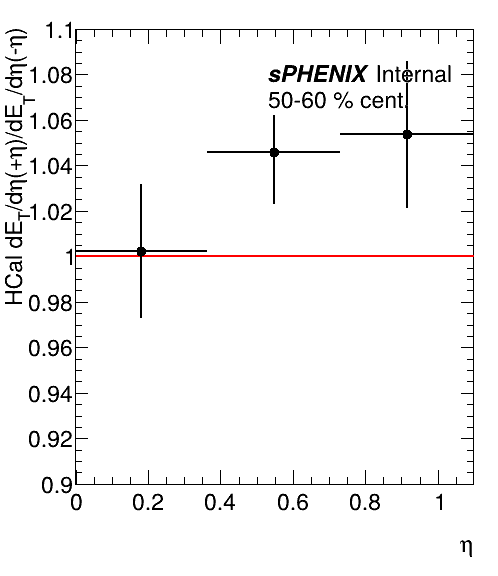
\includegraphics[width=0.32\linewidth]{detdeta/Figures/corr_syst_uncertainties/hcal_eta_ratio_syst_50-60.png}
    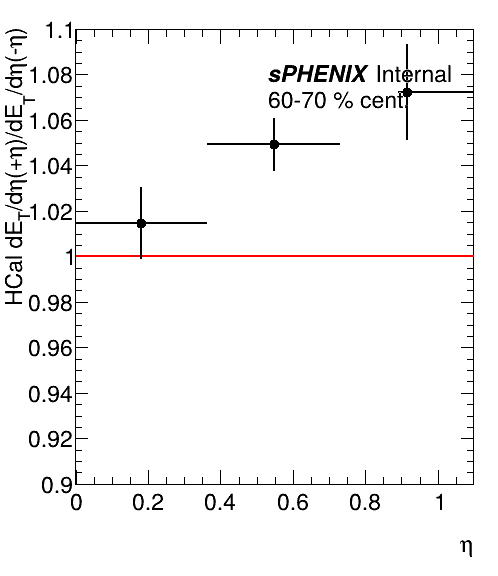
\includegraphics[width=0.32\linewidth]{figures/chapter4/hcal_eta_ratio_syst_60-70.png}
    \caption{Correlation plots for the HCal \detdeta measurements at $0.74 < |\eta| < 1.1$ using each analysis systematic variation for each centrality measurement in the analysis.}
    \label{fig:hcal_eta_detdeta_ratio}
\end{figure}

\end{appendices}
